\chapter{Experiments}
In this chapter we are going to illuminate the feature space of competitive First-Person Shooter maps using a Quality Diversity algorithm.

First, we run some preliminary analysis to understand the noisiness of the simulation-based features and the noisiness of the features extracted from the \textit{SMT-Genome} representation, whose phenotype mapping is not deterministic.

Then we will run a correlation analysis to understand how features correlate with one another, so that we can identify patterns and group features that are highly correlated and reduce the number of features to be examined. We will then look for interesting couples of features that are negatively correlated, as these could be interesting to explore using a QD approach.

Finally, we will use \textit{t-SNE} to visualize the high-dimensional feature space of the maps, the space of the map's images defined by their tiles grid and the space of the map's graph, encoded using a graph embedding method. We will then compare the clustering of the maps in these spaces to understand how features correlate with the visual appearance of the maps and with their topological structure as described by the graph. We will also analyze how the maps' distance in the space projected by \textit{t-SNE} correlates with their features.

Finally, we leverage the insights gained from these analyses to identify three \textit{behavioral characterizations} by selecting relevant couples of features to be illuminated using the \textit{Map-Elites with Sliding Boundaries} algorithm, with the goal of producing maps where gameplay is balanced between bots of differing skill levels. We will then compare the results obtained using different genome representations to understand the differences in their capability to generate varied and balanced designs.

\section{Preliminary analysis}
\subsection{Emergent features noisiness analysis}
\label{subsec:emergent_features_noisiness}
By their very nature, simulations are not deterministic given that bots perform many random actions during a single match. So, while topological features are always the same for a given map, emergent features, such as entropy or pace, may vary. For this reason, we have run an analysis to understand how noisy these features are; if a feature varies too wildly between different matches on the same map, then we may as well consider it random and unfit to describe an actual feature of the examined map.

To gather and visualize this data we have generated a random genome (one for all genome representations discussed in \cref{sec:map_genomes}), converted it to a phenotype and run 100 different matches on the same map, recording the emergent features at the end of each match. Each feature has thus 100 data points which have been used to draw a boxplot\footnote{\url{https://pandas.pydata.org/docs/reference/api/pandas.DataFrame.boxplot.html}}, which allows us to neatly visualize the distribution (median, first and third quartile, maximum, minimum and outliers) of the data. While some features, such as entropy or pace, have a maximum and minimum possible value, others, such as the maximum value of the heatmaps, do not. In order to visualize and compare features we have normalized all features to the range $[0, 1]$, using the empirical minimum and maximum values, obtained from roughly 16000 matches on different maps, when needed. The results are shown in figures \cref{fig:emergent_features_noisiness_ab}, \cref{fig:emergent_features_noisiness_grid}, \cref{fig:emergent_features_noisiness_pointad} and \cref{fig:emergent_features_noisiness_smt}.

\begin{figure}[p]
    \centering
    \subfloat{

        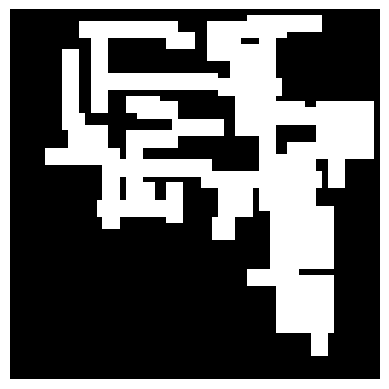
\includegraphics[width=0.15\textwidth, valign=c]{images/phenotype_var_ab_0_nm1.png}
        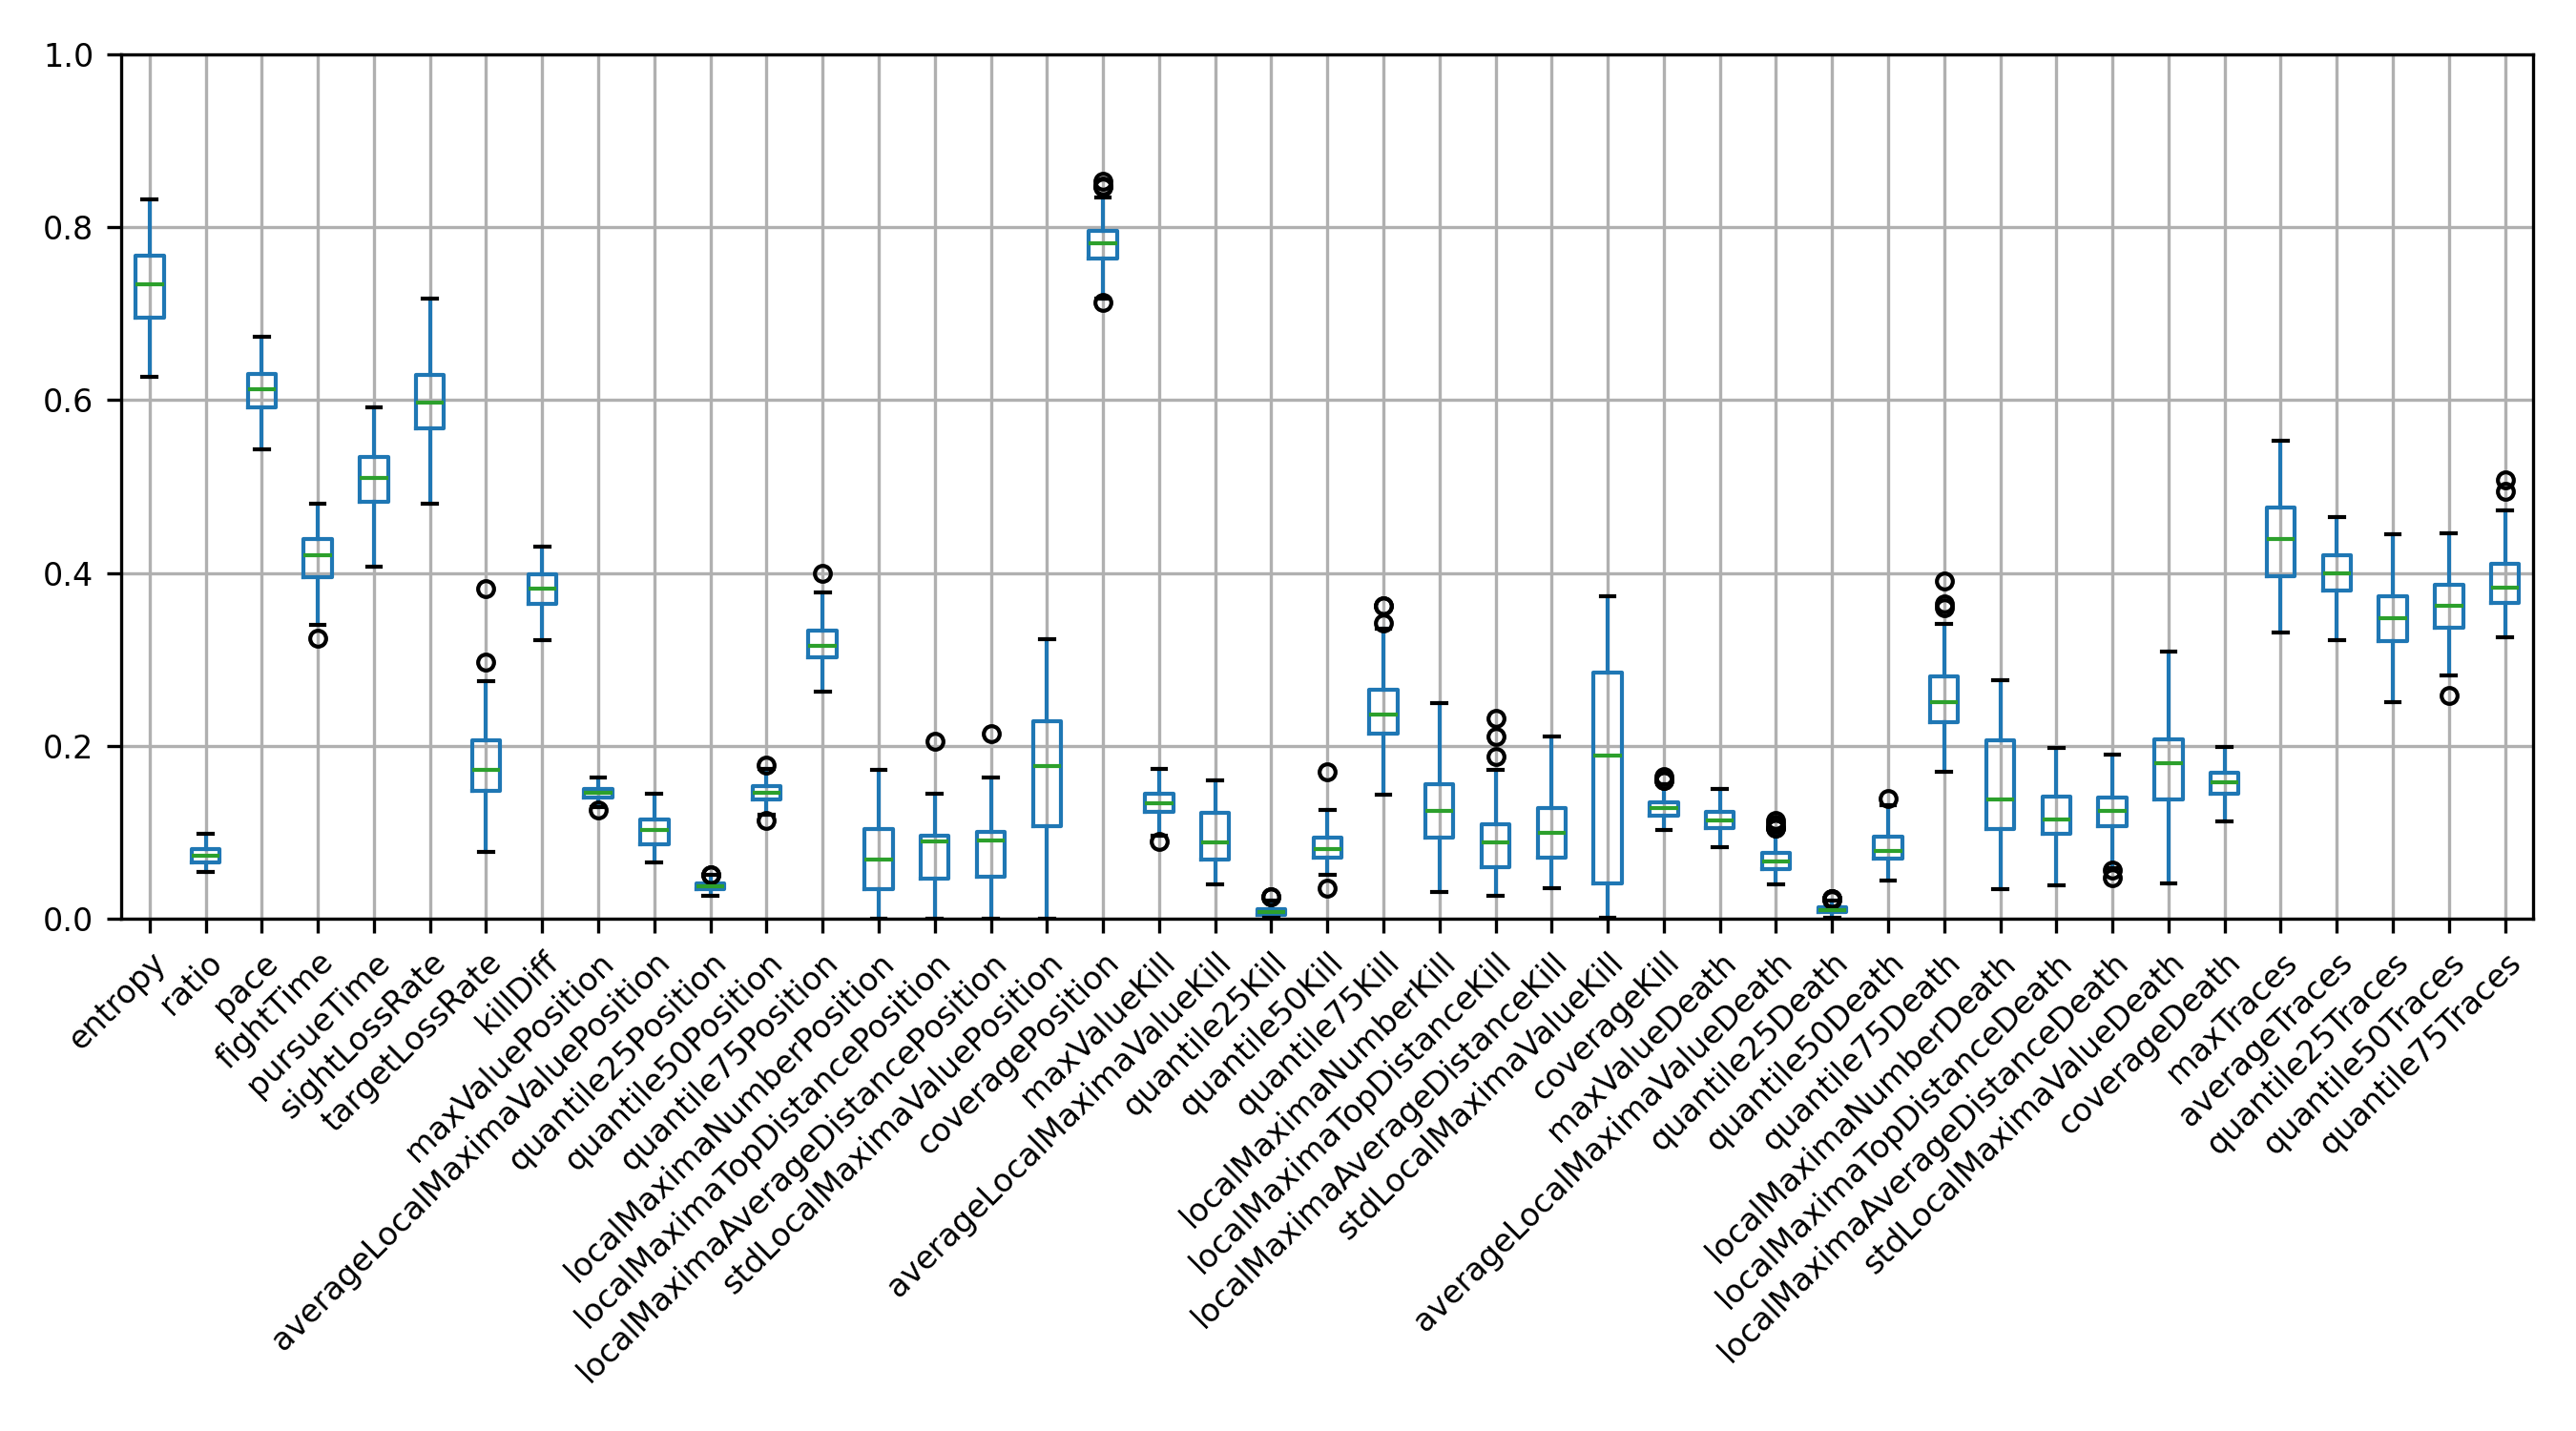
\includegraphics[width=0.85\textwidth, valign=c]{images/boxplot_var_ab_0_nm1_numsim_1.png}
        }
    \caption{Boxplot of emergent features for a random \textit{All-Black} phenotype.}
    \label{fig:emergent_features_noisiness_ab}
\end{figure}
\begin{figure}[p]
    \centering
    \subfloat{
        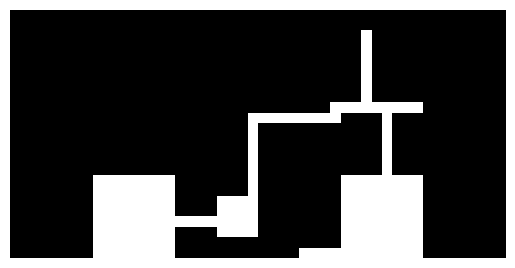
\includegraphics[width=0.15\textwidth, valign=c]{images/phenotype_var_grid_0_nm1.png}
        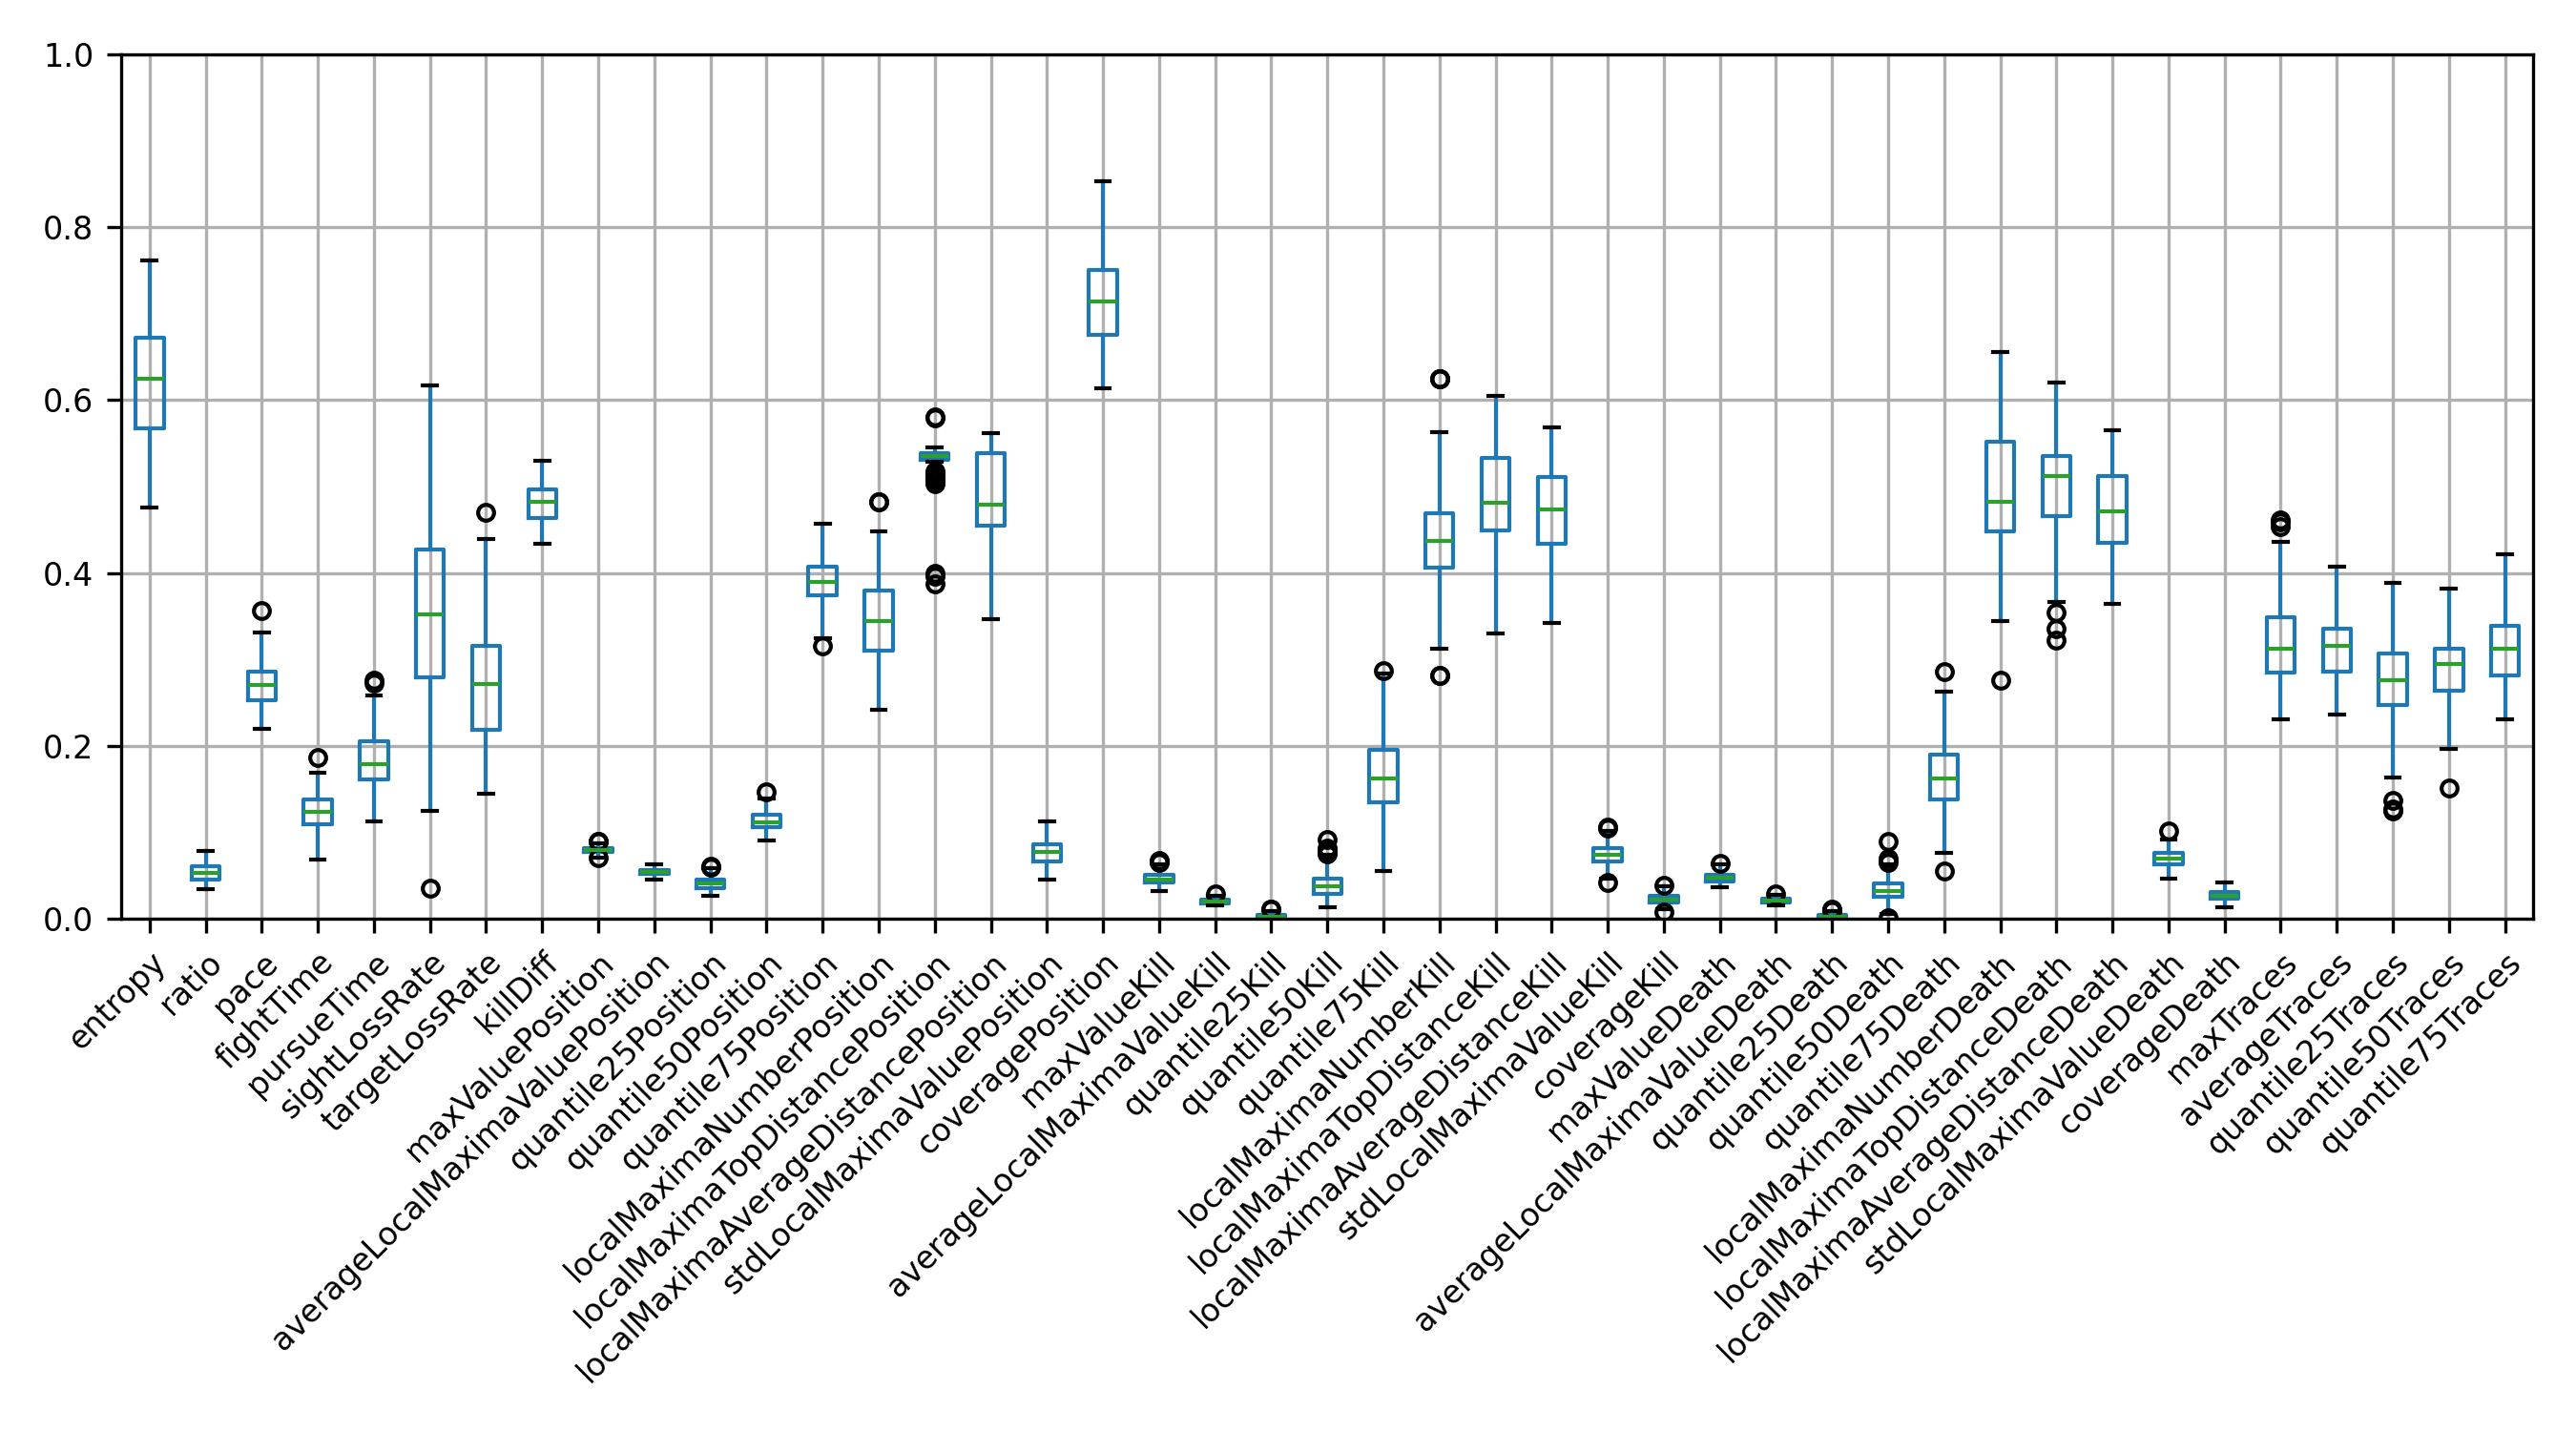
\includegraphics[width=0.85\textwidth, valign=c]{images/boxplot_var_grid_0_nm1_numsim_1.png}
        }
    \caption{Boxplot of emergent features for a random \textit{Grid-Graph} phenotype.}
    \label{fig:emergent_features_noisiness_grid}
\end{figure}
\begin{figure}[p]
    \centering
    \subfloat{
        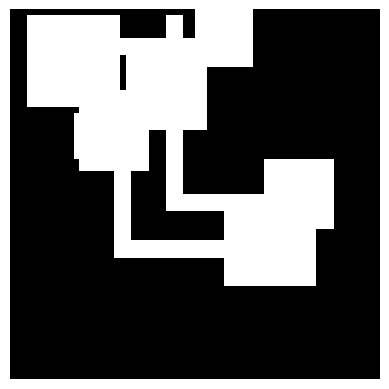
\includegraphics[width=0.15\textwidth, valign=c]{images/phenotype_var_pointad_0_nm1.png}
        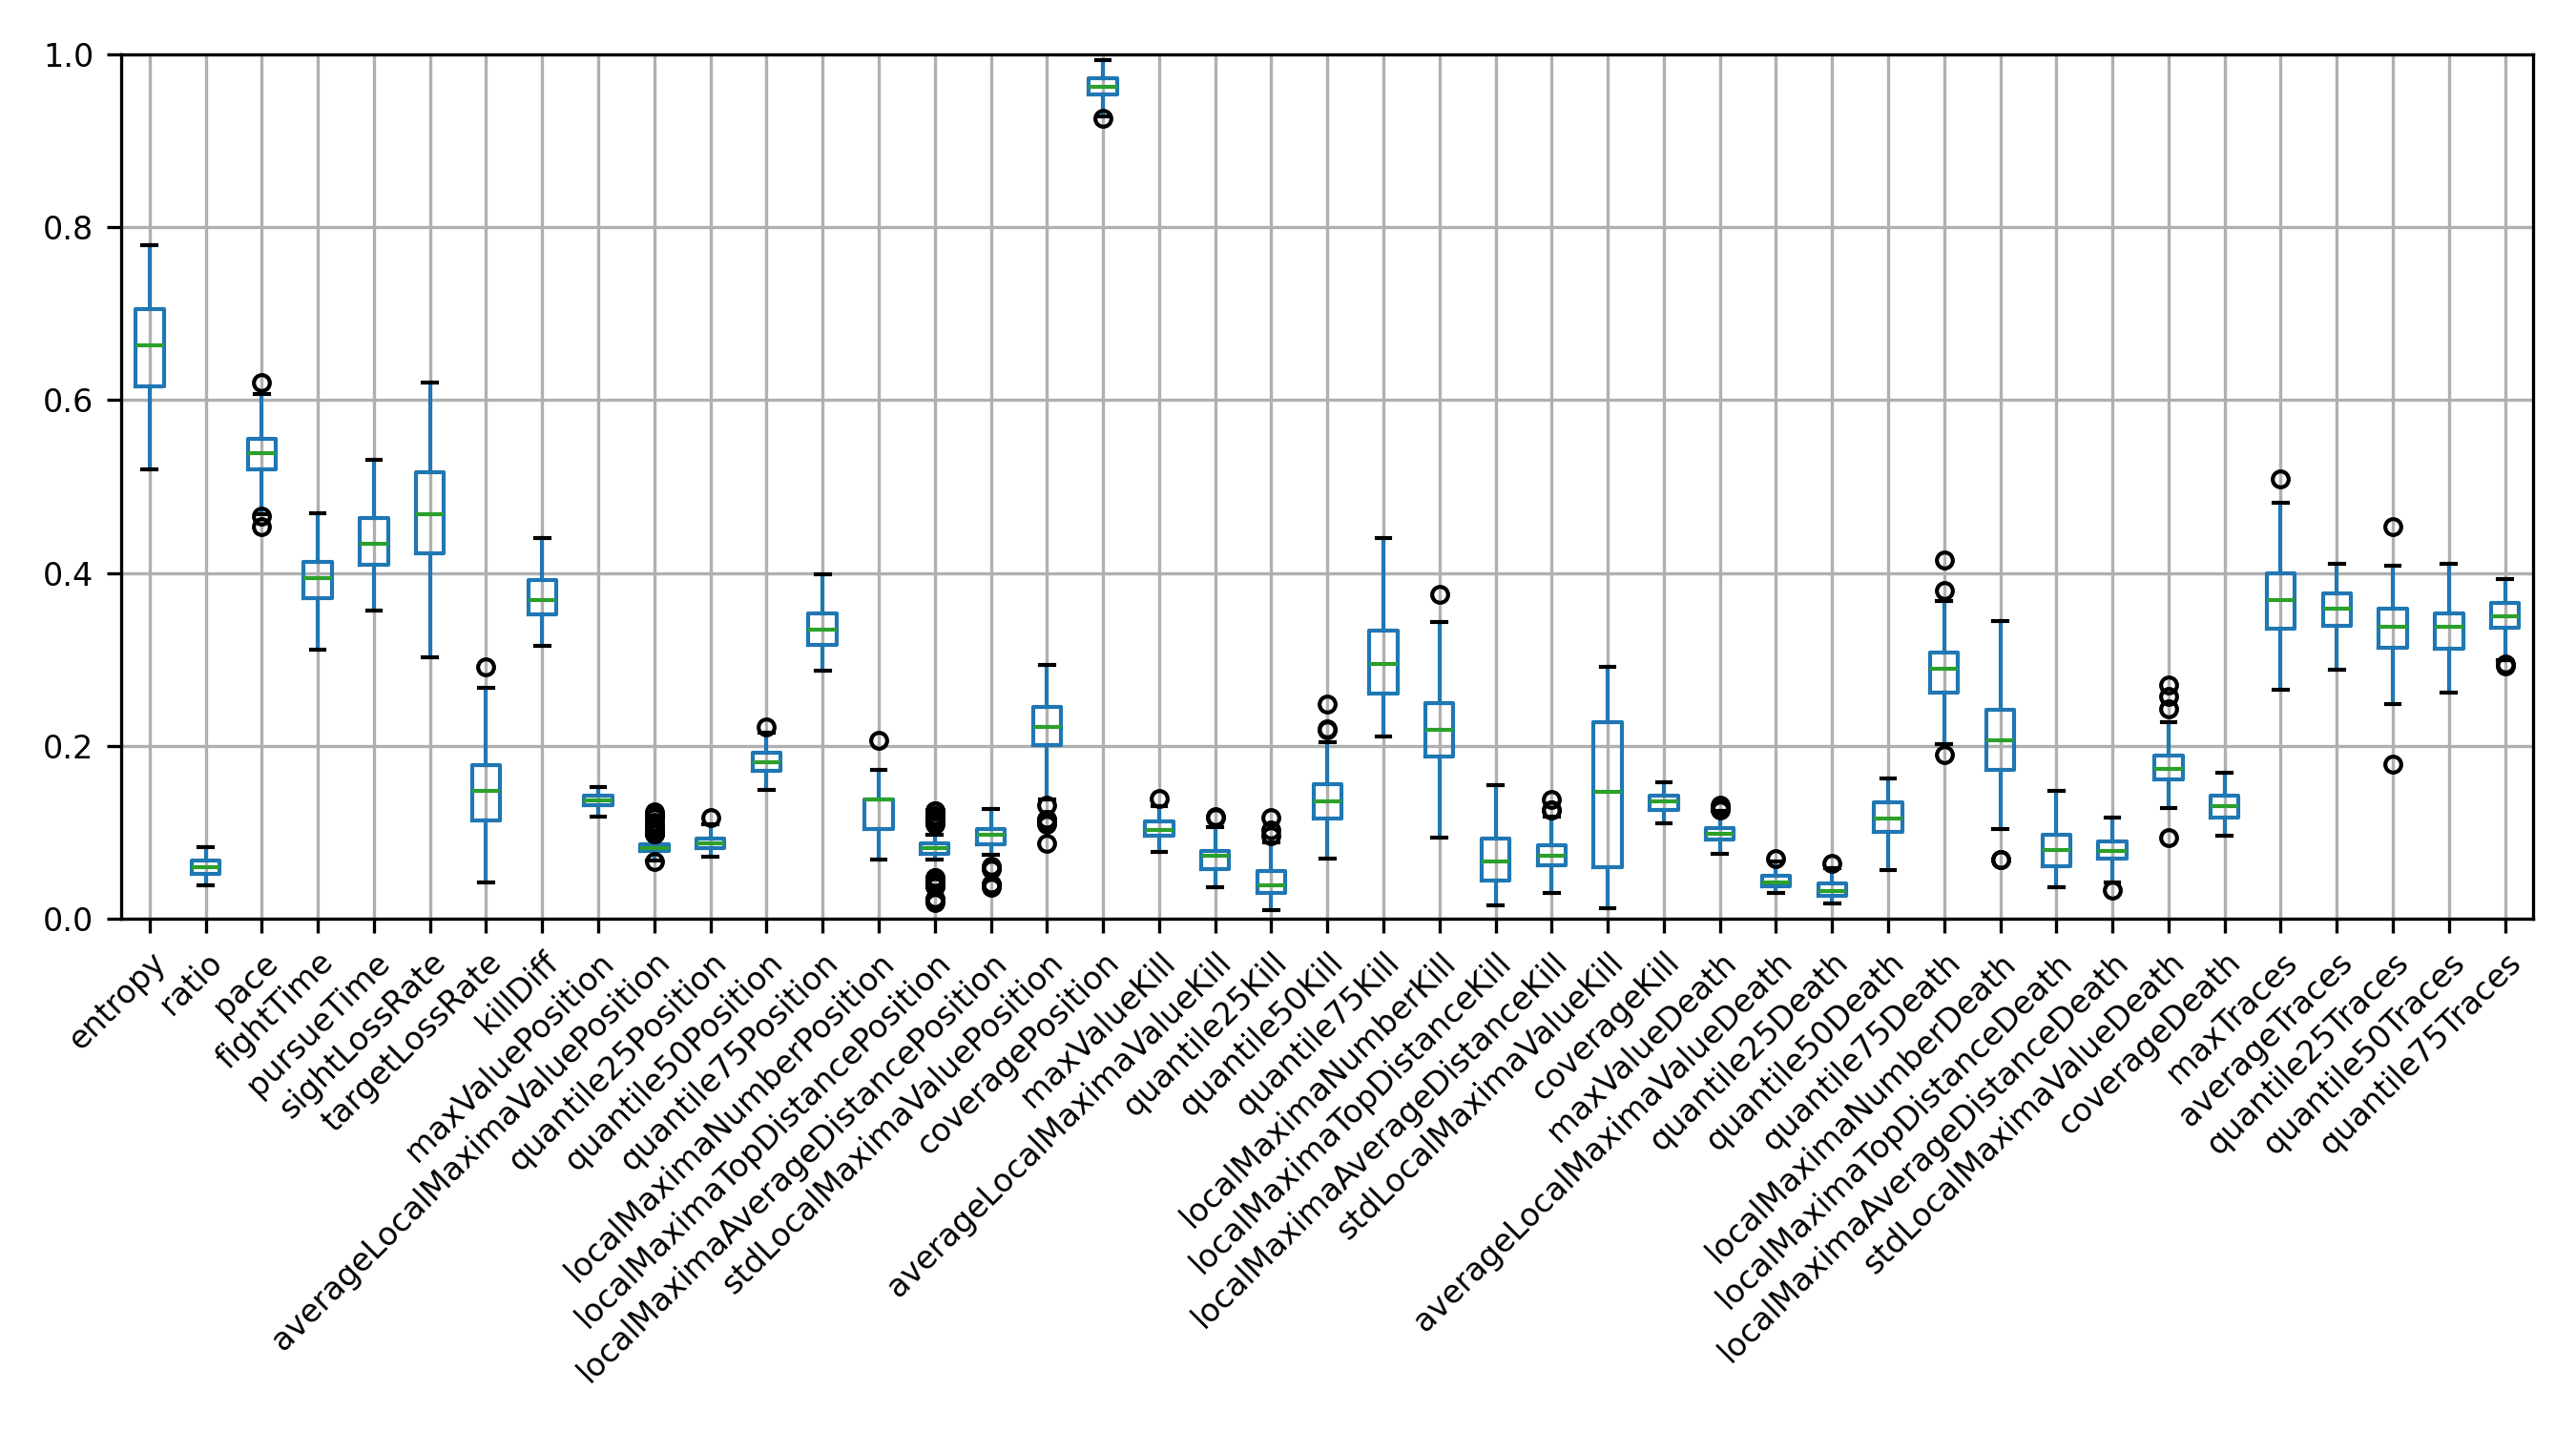
\includegraphics[width=0.85\textwidth, valign=c]{images/boxplot_var_pointad_0_nm1_numsim_1.png}
    }
    \caption{Boxplot of emergent features for a random Point-Line phenotype.}
    \label{fig:emergent_features_noisiness_pointad}
\end{figure}
\begin{figure}[p]
    \centering
    \subfloat{
        
        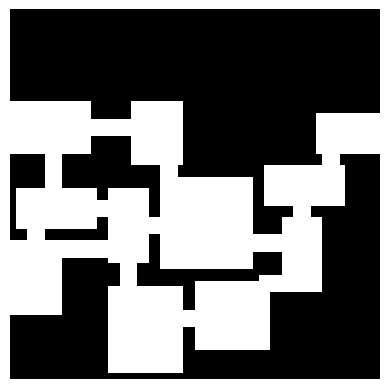
\includegraphics[width=0.15\textwidth, valign=c]{images/phenotype_var_smt_0_nm1.png}
        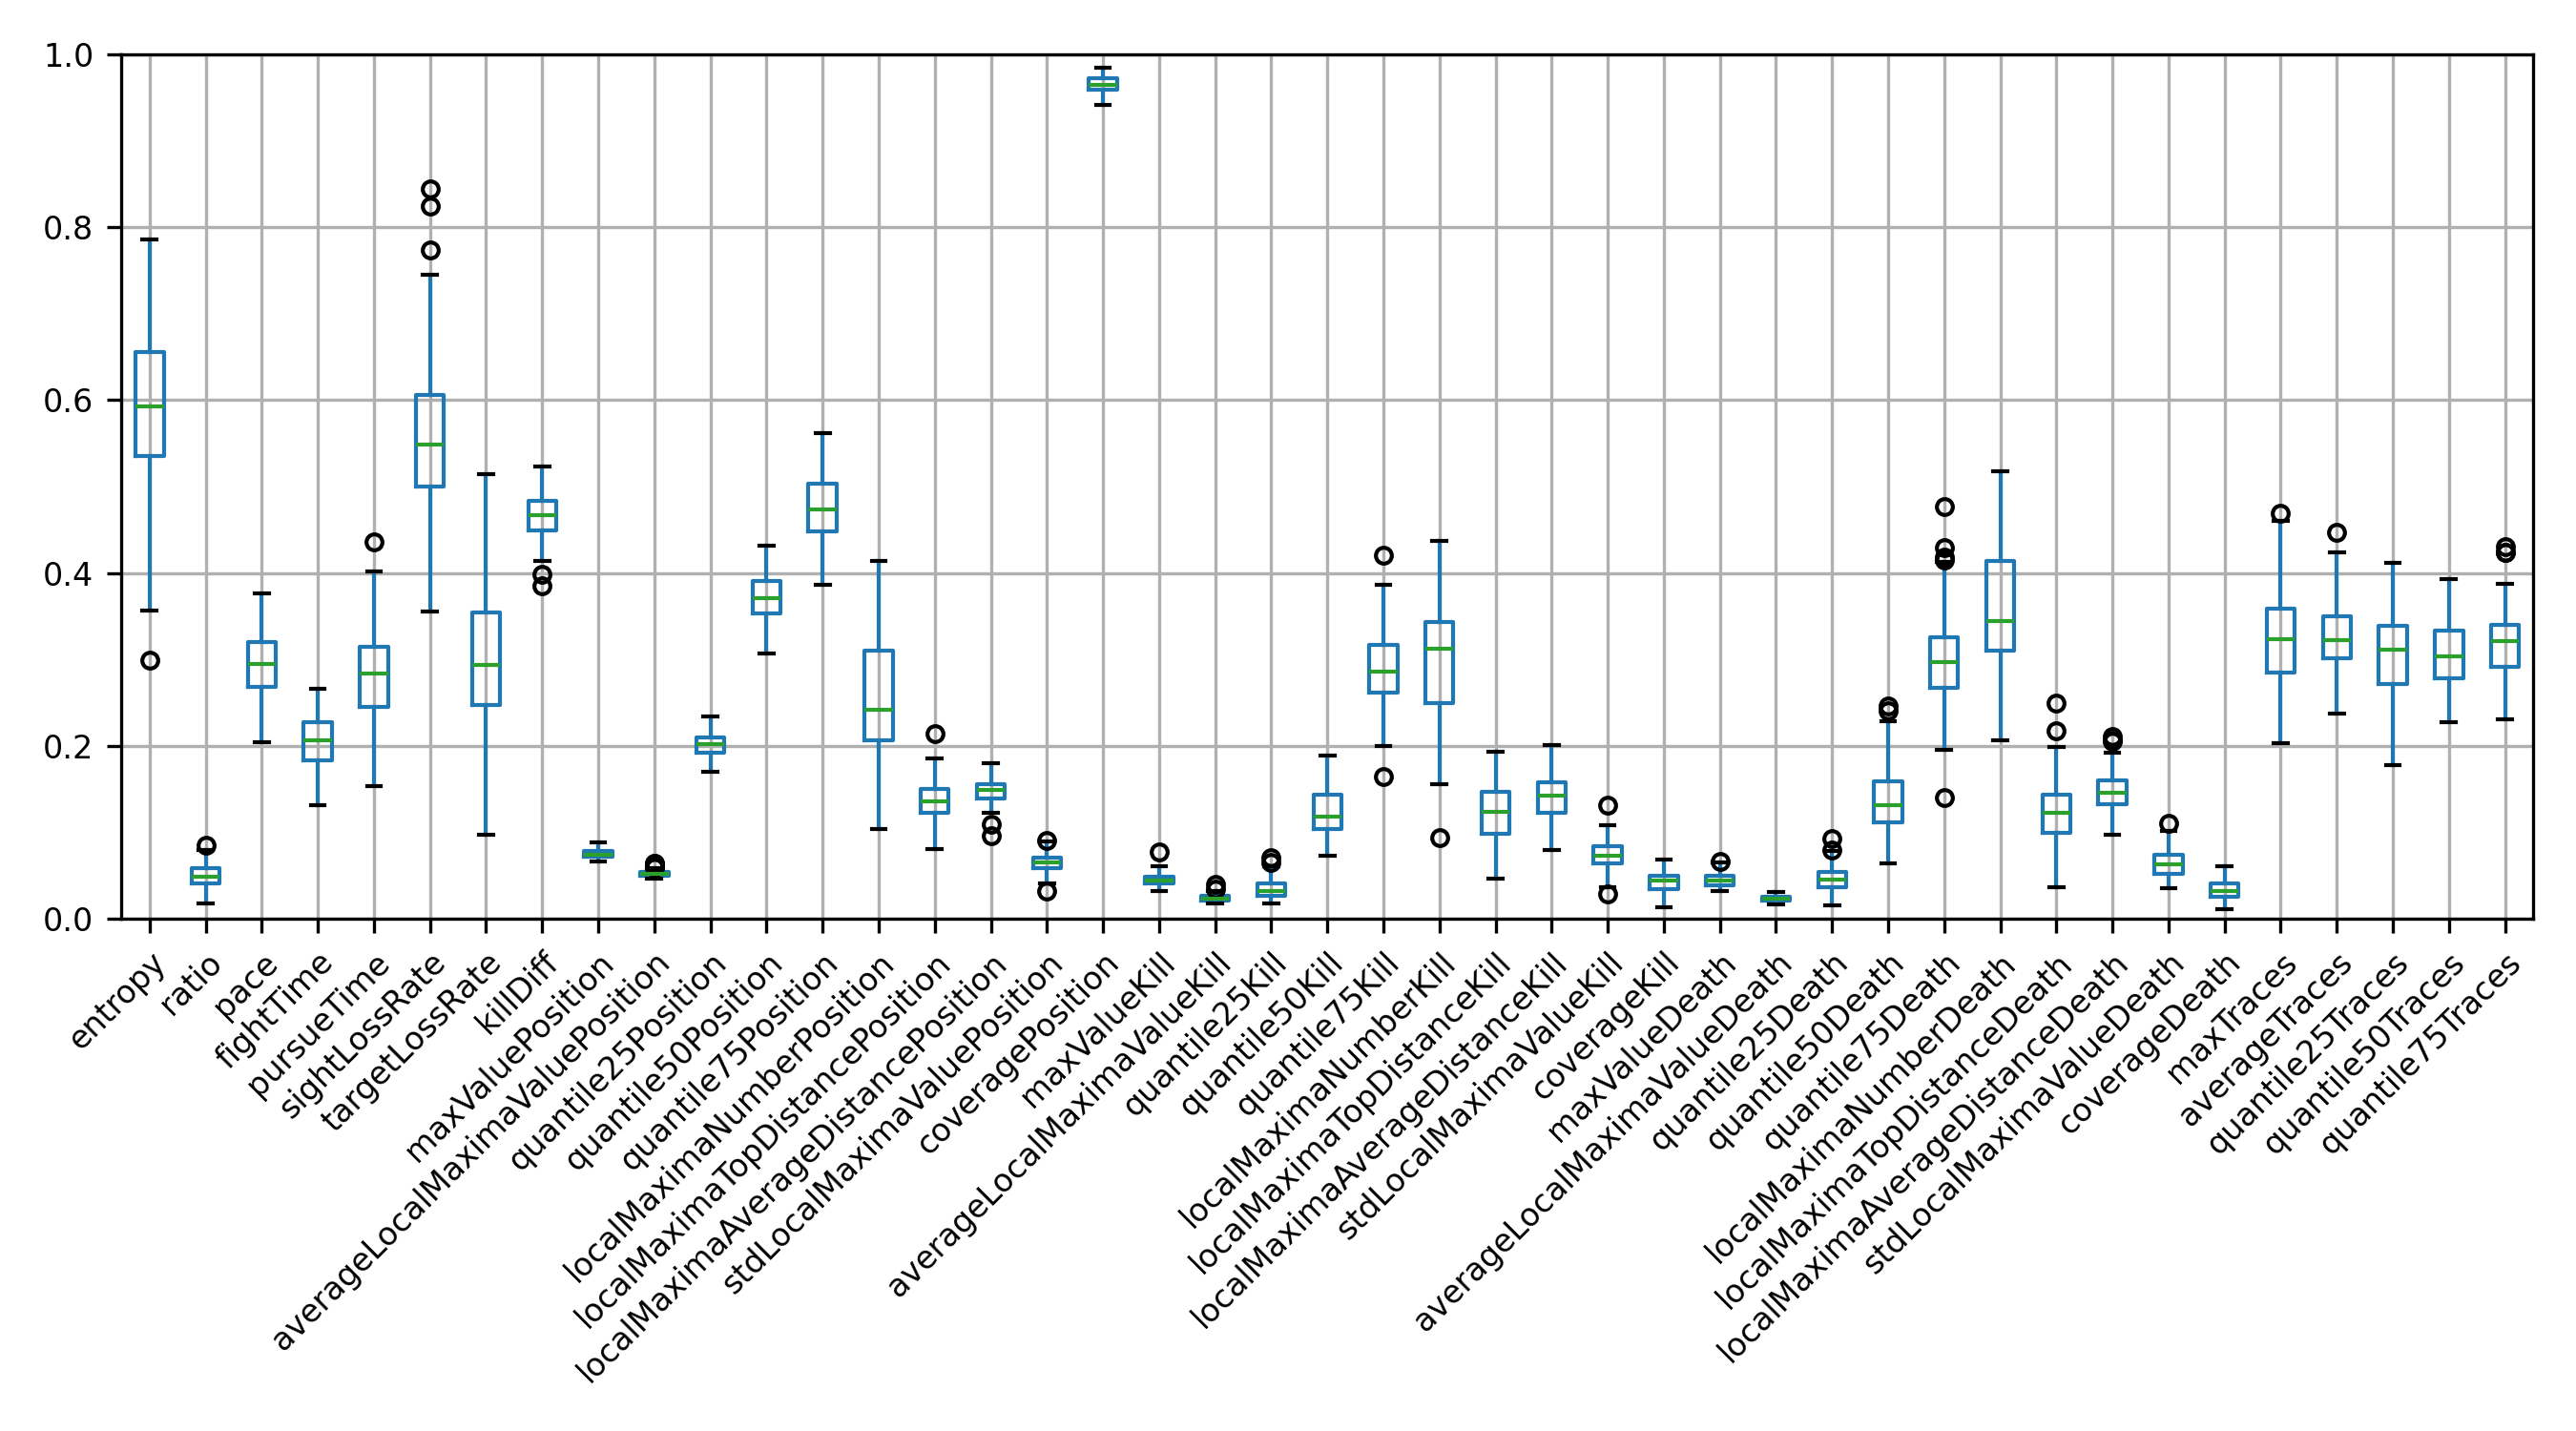
\includegraphics[width=0.85\textwidth, valign=c]{images/boxplot_var_smt_0_nm1_numsim_1.png}
    }
    \caption{Boxplot of emergent features for a random SMT phenotype.}
    \label{fig:emergent_features_noisiness_smt}
\end{figure}

\clearpage
We notice that results do not differ significantly between different genomes. We can also conclude that, while some features are occasionally noisier (e.g. stdLocalMaximaValueKill in \cref{fig:emergent_features_noisiness_ab}, sightLossRate in \cref{fig:emergent_features_noisiness_grid} and entropy in \cref{fig:emergent_features_noisiness_smt}), in general all have a reasonable and similar amount of noise. To improve our results, we believe that averaging the features over multiple matches would be beneficial. To this end, we repeated the analysis by averaging the features over 5 matches, obtaining again 100 data points for each feature, where each data point is the average of the result of 5 matches. The results are shown in figures \cref{fig:emergent_features_noisiness_5_ab}, \cref{fig:emergent_features_noisiness_5_grid}, \cref{fig:emergent_features_noisiness_5_pointad} and \cref{fig:emergent_features_noisiness_5_smt}.

\vspace*{\fill}
{
\centering
\begin{figure}[hbt!]
    \centering
    \subfloat{ 
        \centering
        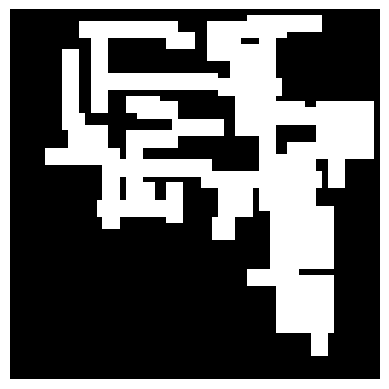
\includegraphics[width=0.15\textwidth, valign=c]{images/phenotype_var_ab_0_nm5.png}
        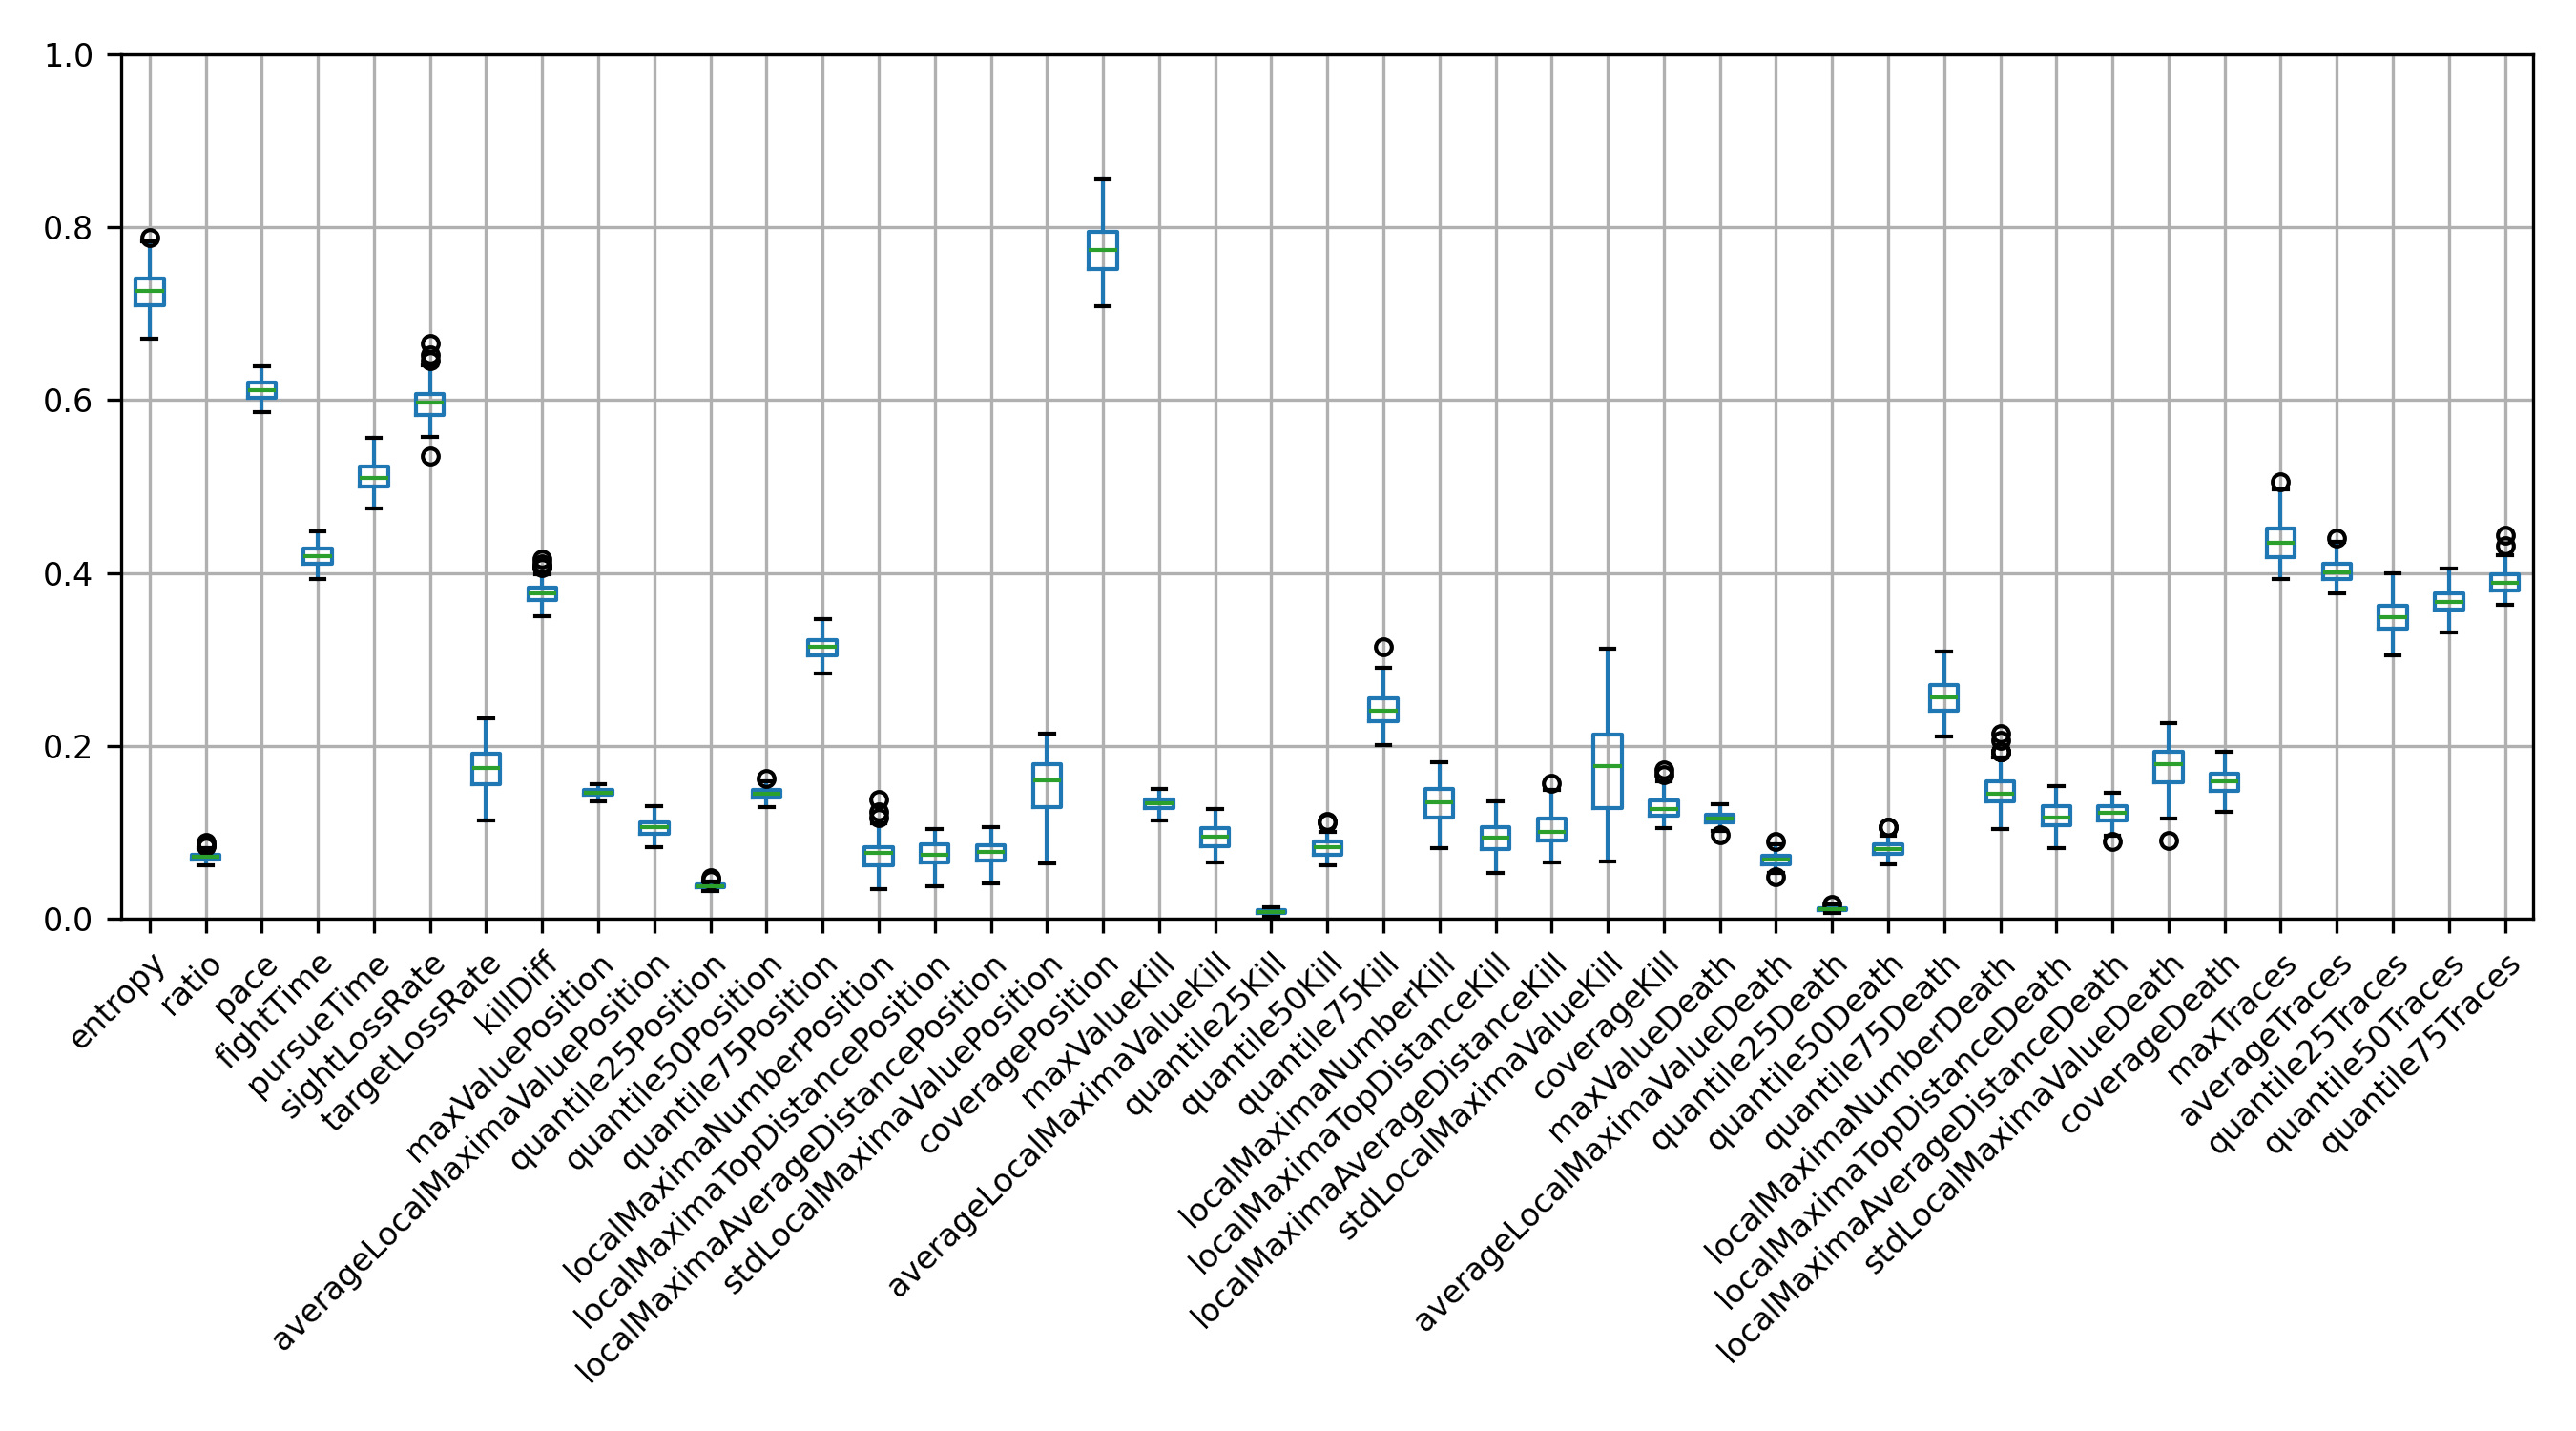
\includegraphics[width=0.85\textwidth, valign=c]{images/boxplot_var_ab_0_nm5_numsim_5.png}
    }
    \caption{Boxplot of emergent features for a random \textit{All-Black} phenotype averaging 5 matches.}
    \label{fig:emergent_features_noisiness_5_ab}
\end{figure}
}
\vspace*{\fill}
\begin{figure}[p]
    \subfloat{ 
        \centering
        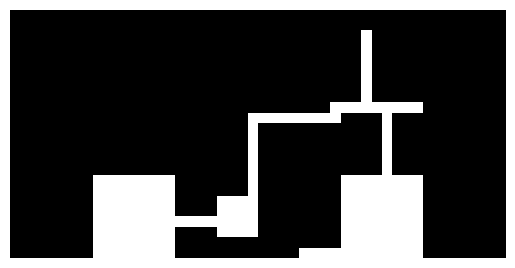
\includegraphics[width=0.15\textwidth, valign=c]{images/phenotype_var_grid_0_nm5.png}
        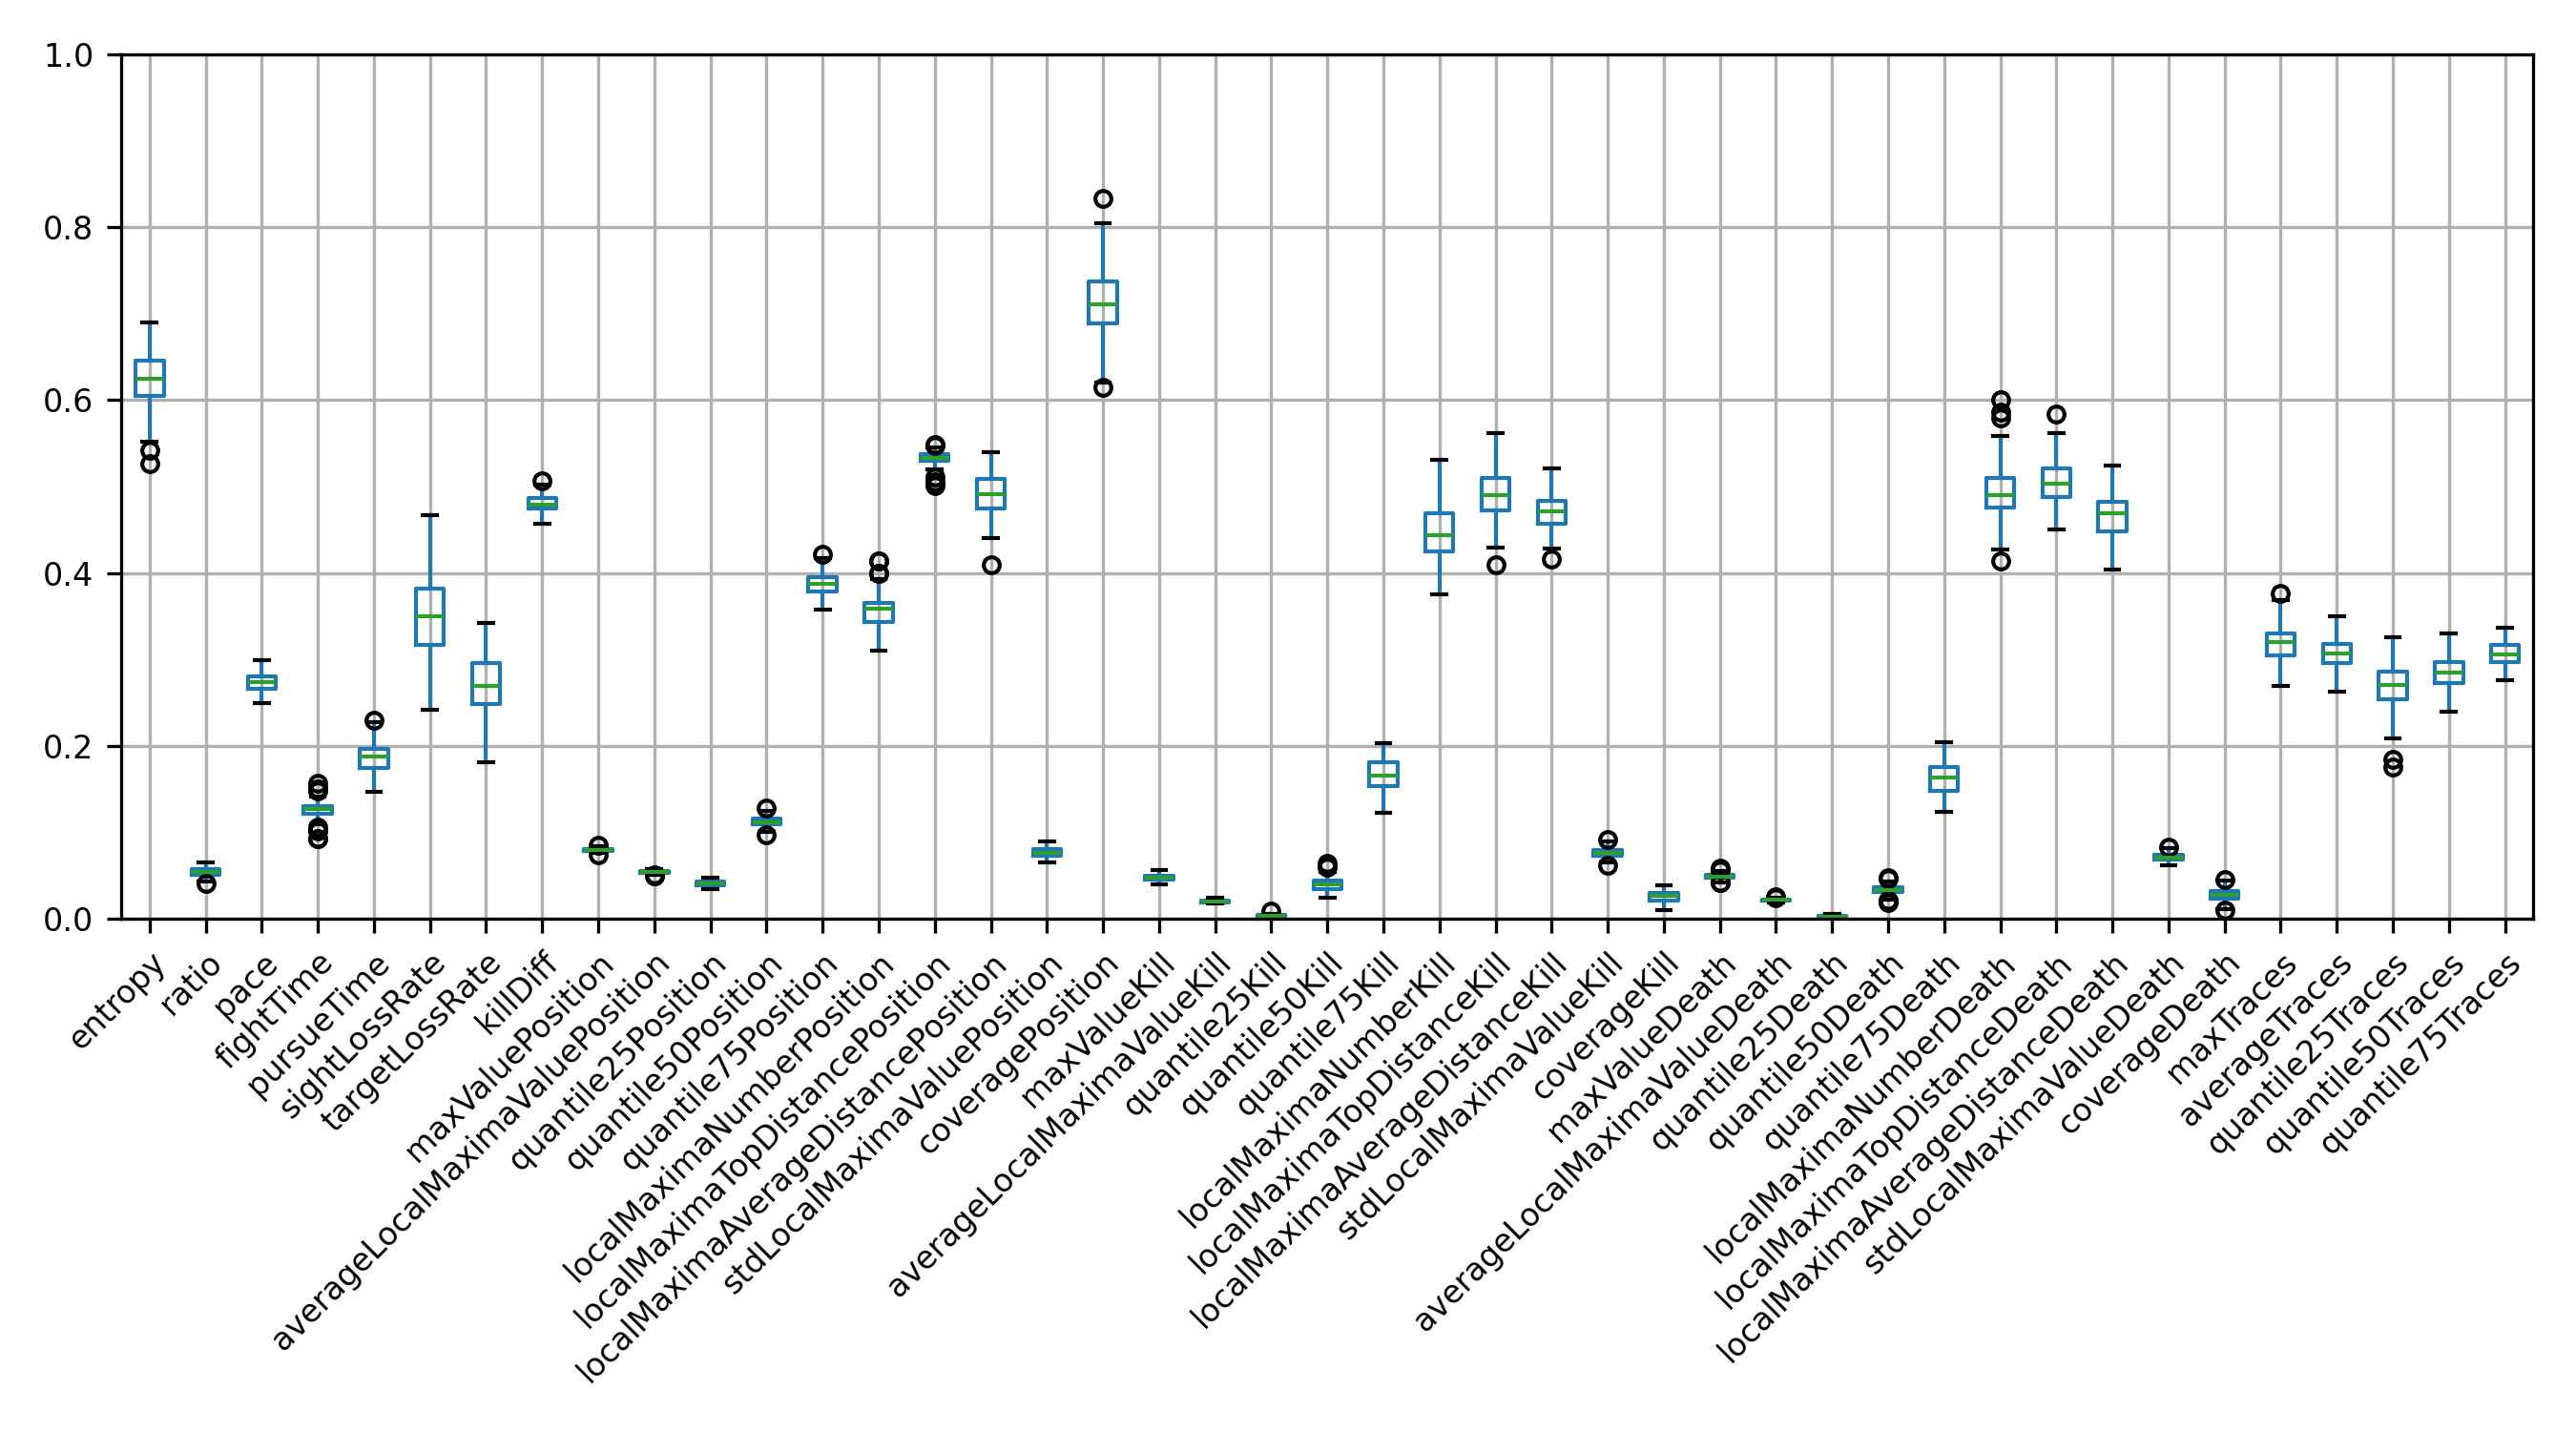
\includegraphics[width=0.85\textwidth, valign=c]{images/boxplot_var_grid_0_nm5_numsim_5.png}
        }
    \caption{Boxplot of emergent features for a random \textit{Grid-Graph} phenotype averaging 5 matches.}
    \label{fig:emergent_features_noisiness_5_grid}
\end{figure}

\begin{figure}[p]
    \subfloat{
        \centering
        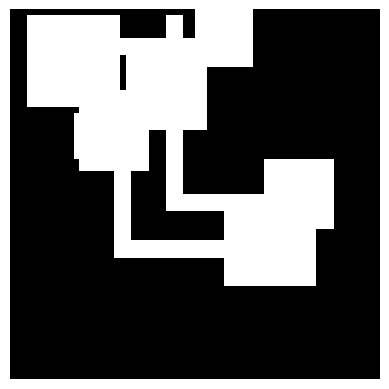
\includegraphics[width=0.15\textwidth, valign=c]{images/phenotype_var_pointad_0_nm5.png}
        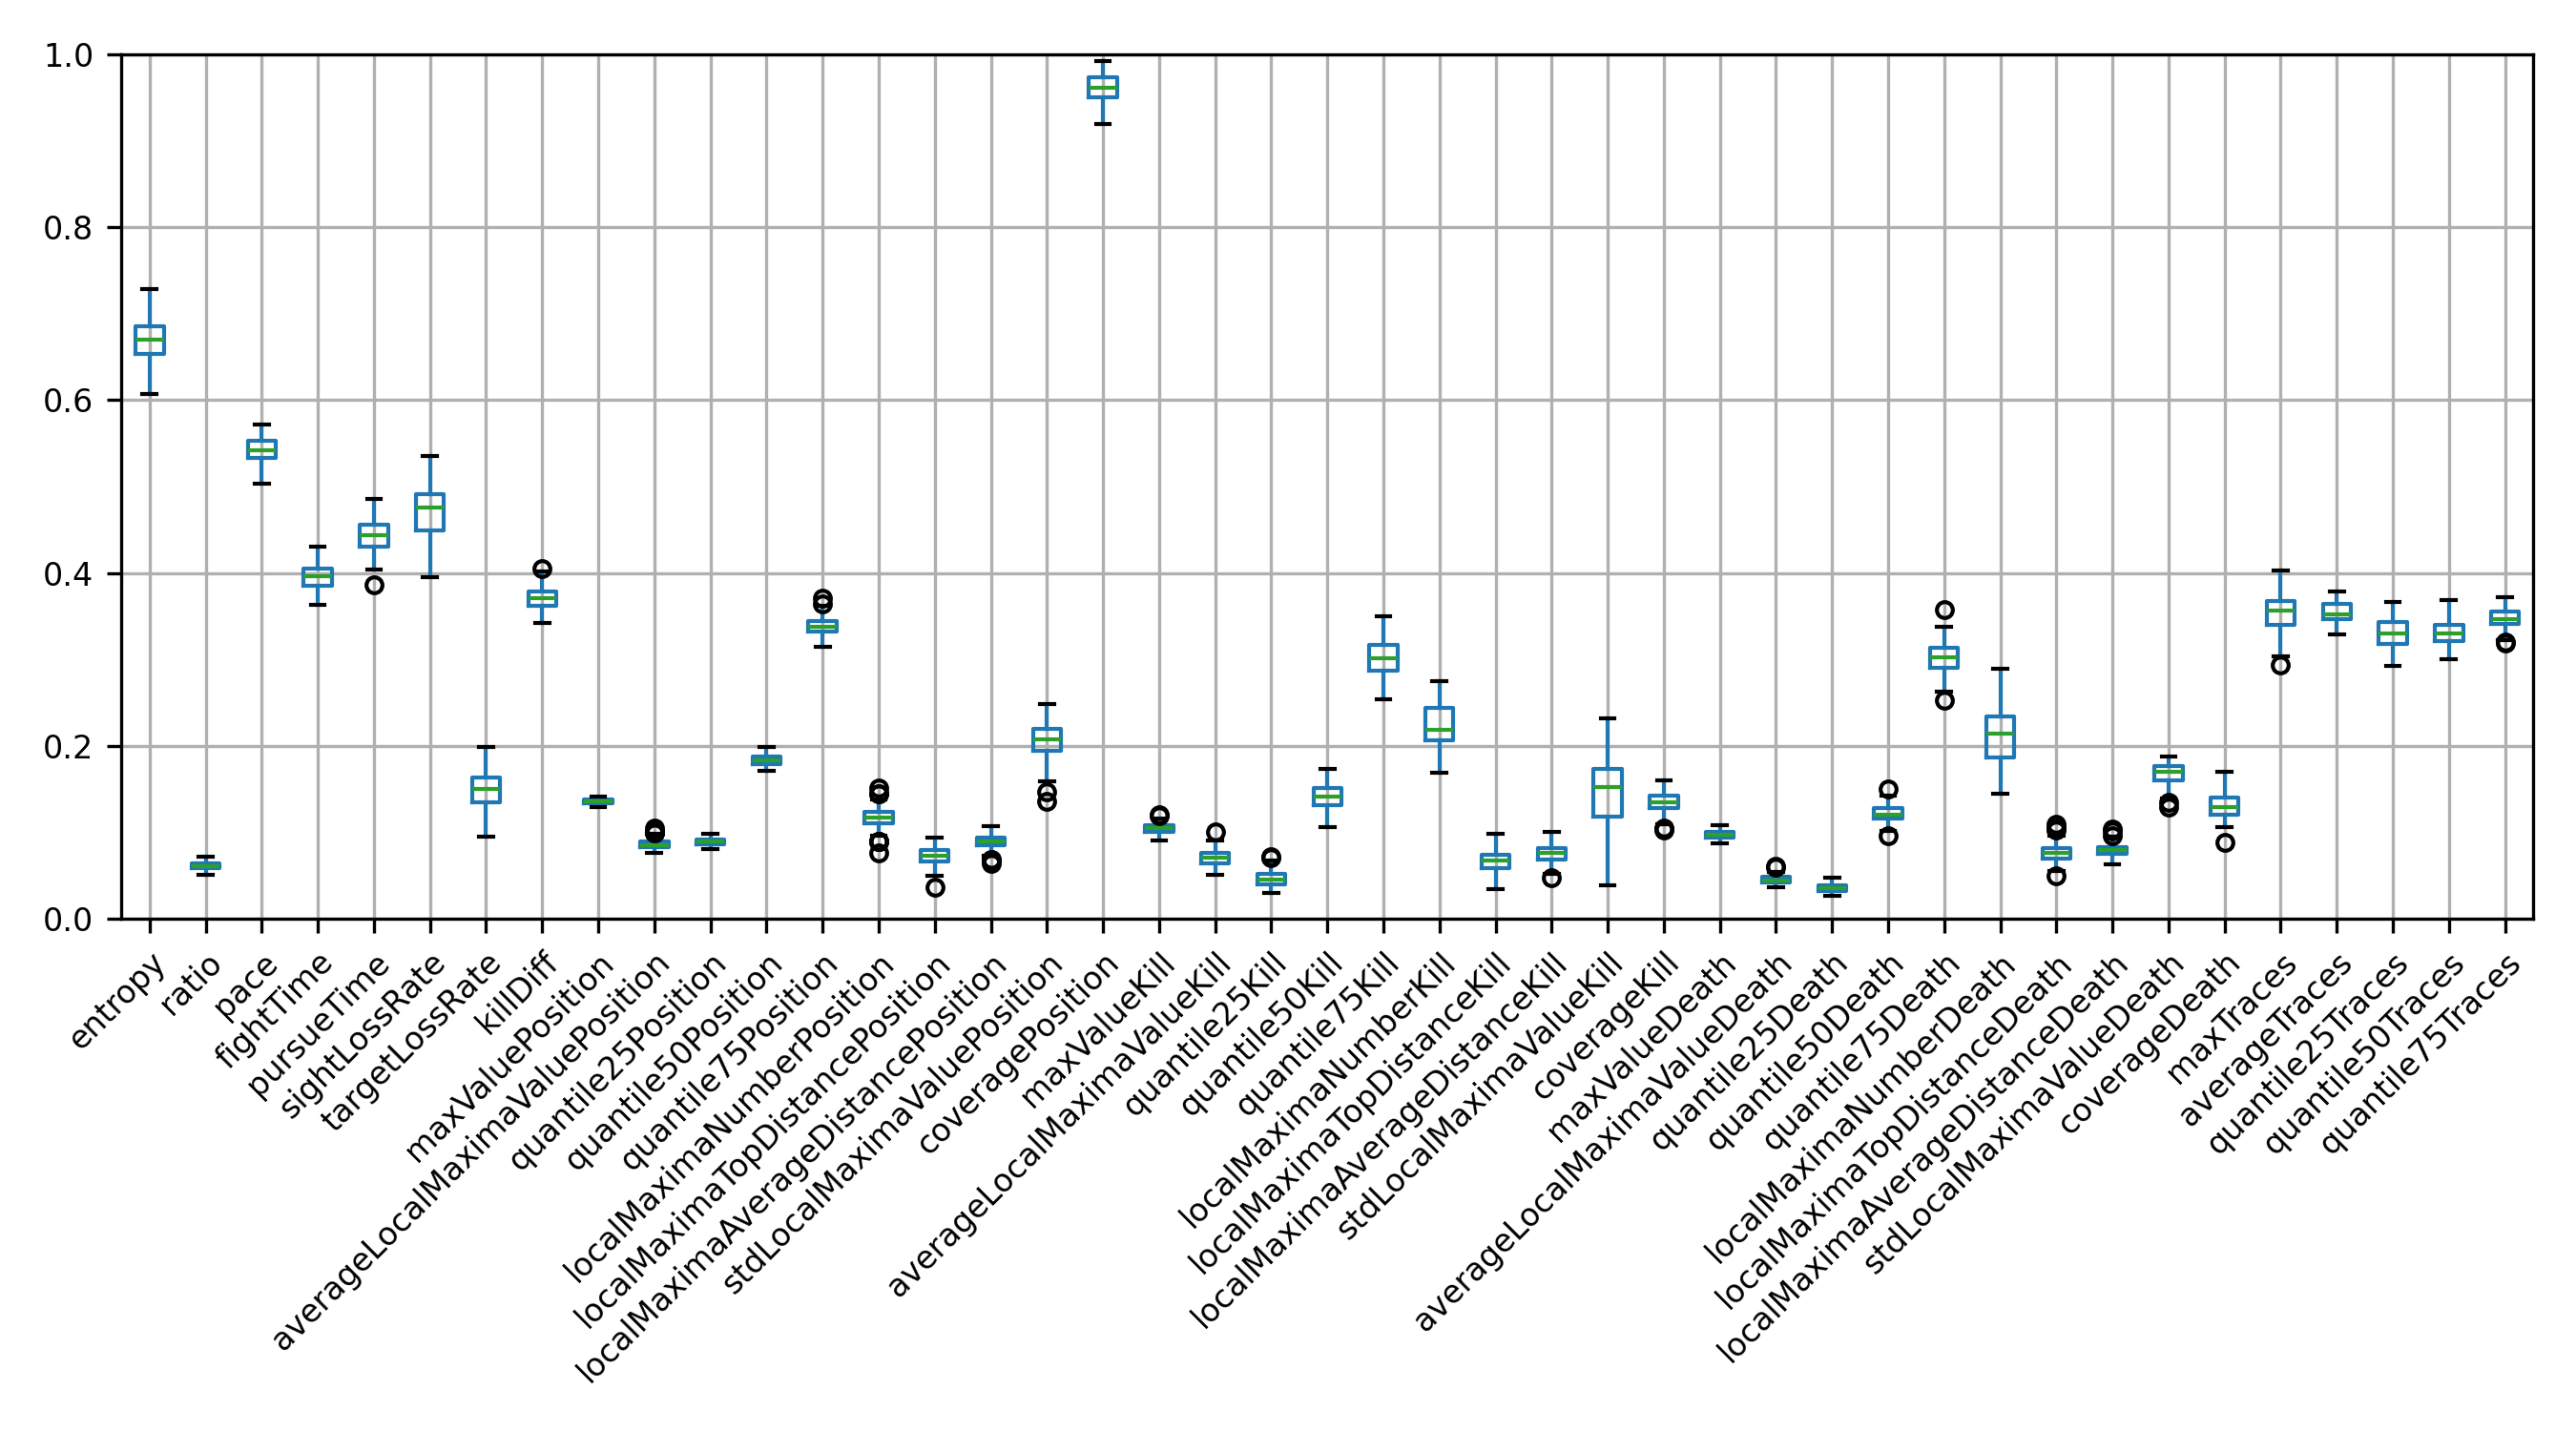
\includegraphics[width=0.85\textwidth, valign=c]{images/boxplot_var_pointad_0_nm5_numsim_5.png}
    }
    \caption{Boxplot of emergent features for a random Point-Line phenotype averaging 5 matches.}
    \label{fig:emergent_features_noisiness_5_pointad}
\end{figure}
\begin{figure}[H]
    \subfloat{ 
        \centering
        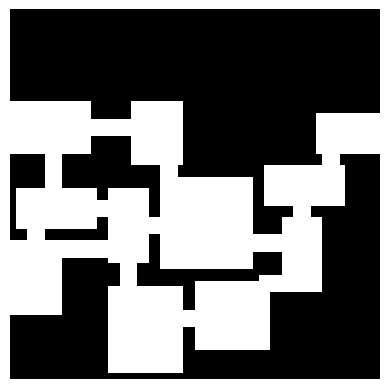
\includegraphics[width=0.15\textwidth, valign=c]{images/phenotype_var_smt_0_nm5.png}
        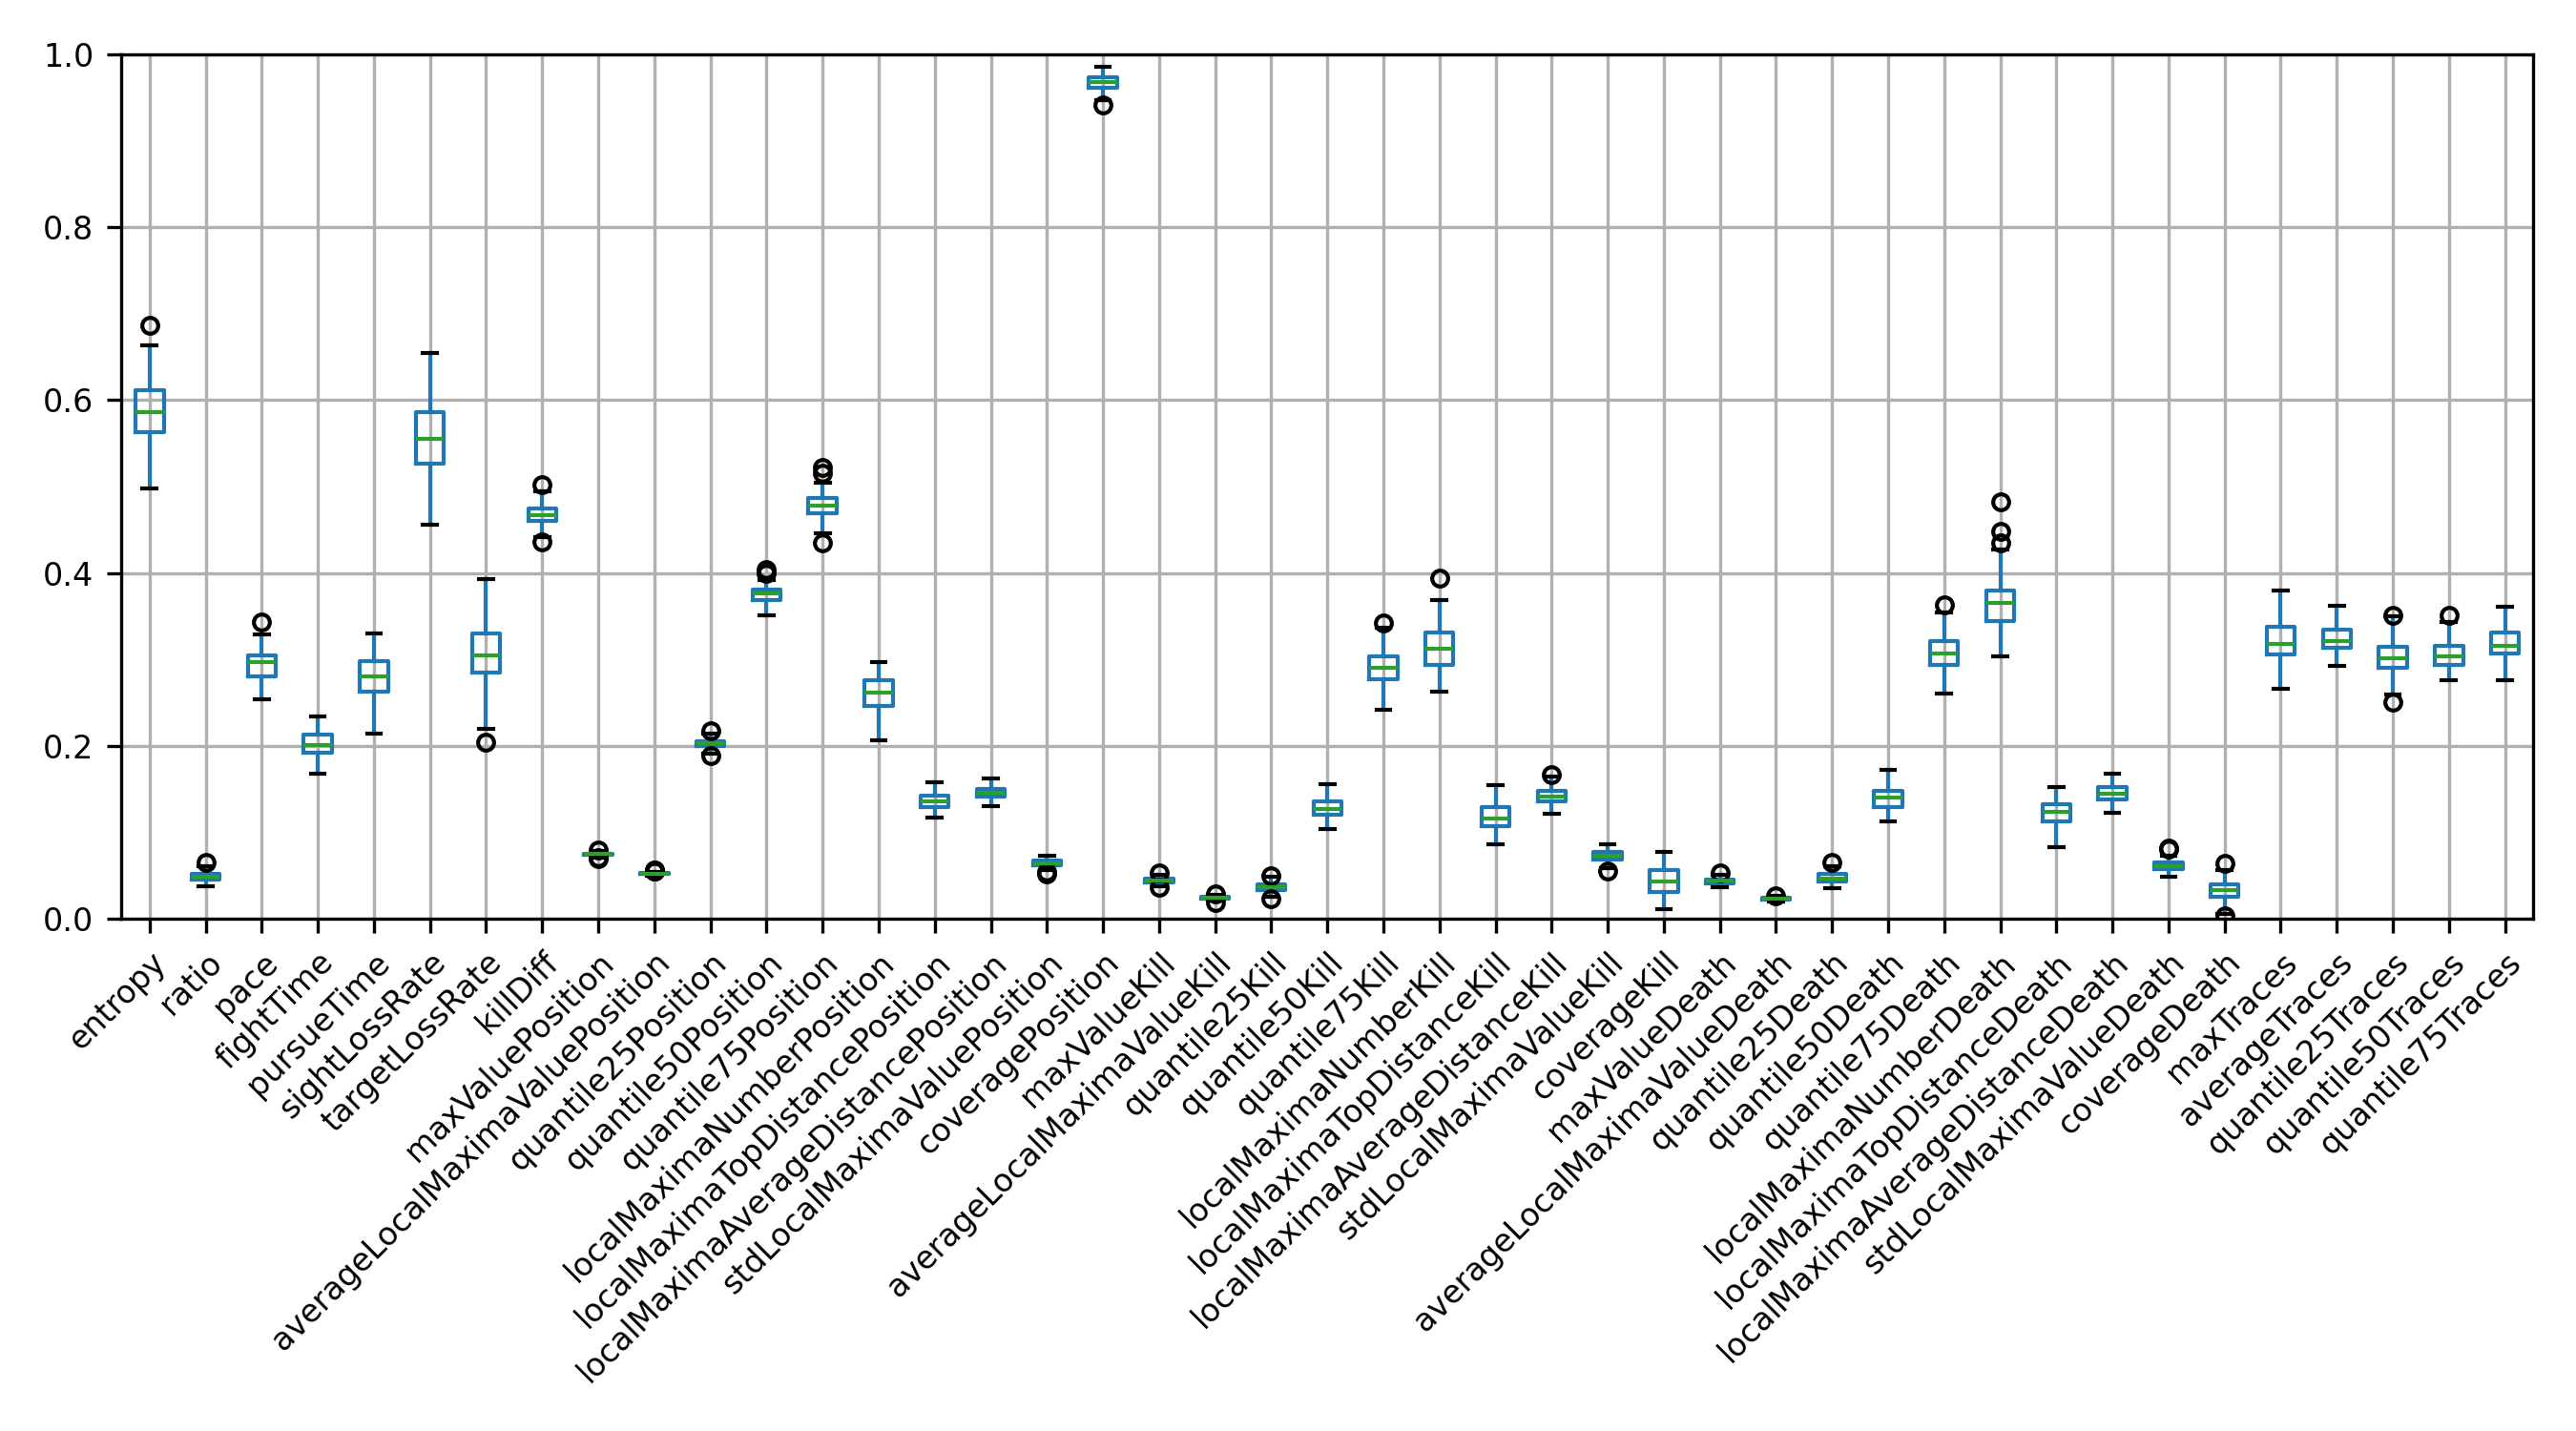
\includegraphics[width=0.85\textwidth, valign=c]{images/boxplot_var_smt_0_nm5_numsim_5.png}
    }
    \caption{Boxplot of emergent features for a random SMT phenotype averaging 5 matches.}
    \label{fig:emergent_features_noisiness_5_smt}
\end{figure}


As expected, the results are even less noisy, and suggest that all metrics are suitable to describe maps. 

\subsection{SMT-Genome phenotype mapping analysis}
\label{subsec:smt_genome_phenotype_mapping}
As we highlighted in \cref{subsec:smt_genome}, the SMT-Genome is not deterministic, meaning that the same genome could lead to different map layouts when mapped to a phenotype. In this section we determine the noisiness of an SMT-Genome by generating 200 phenotypes from the same genome and calculating both emergent and topological features by simulating 5 matches and averaging results. The 200 data-points are used to draw a boxplot for each feature, which is shown in figures \cref{fig:smt_genome_noisiness_emergent} and \cref{fig:smt_genome_noisiness_topology}.

\begin{figure}[hbt!]
    \centering
    \subfloat{
        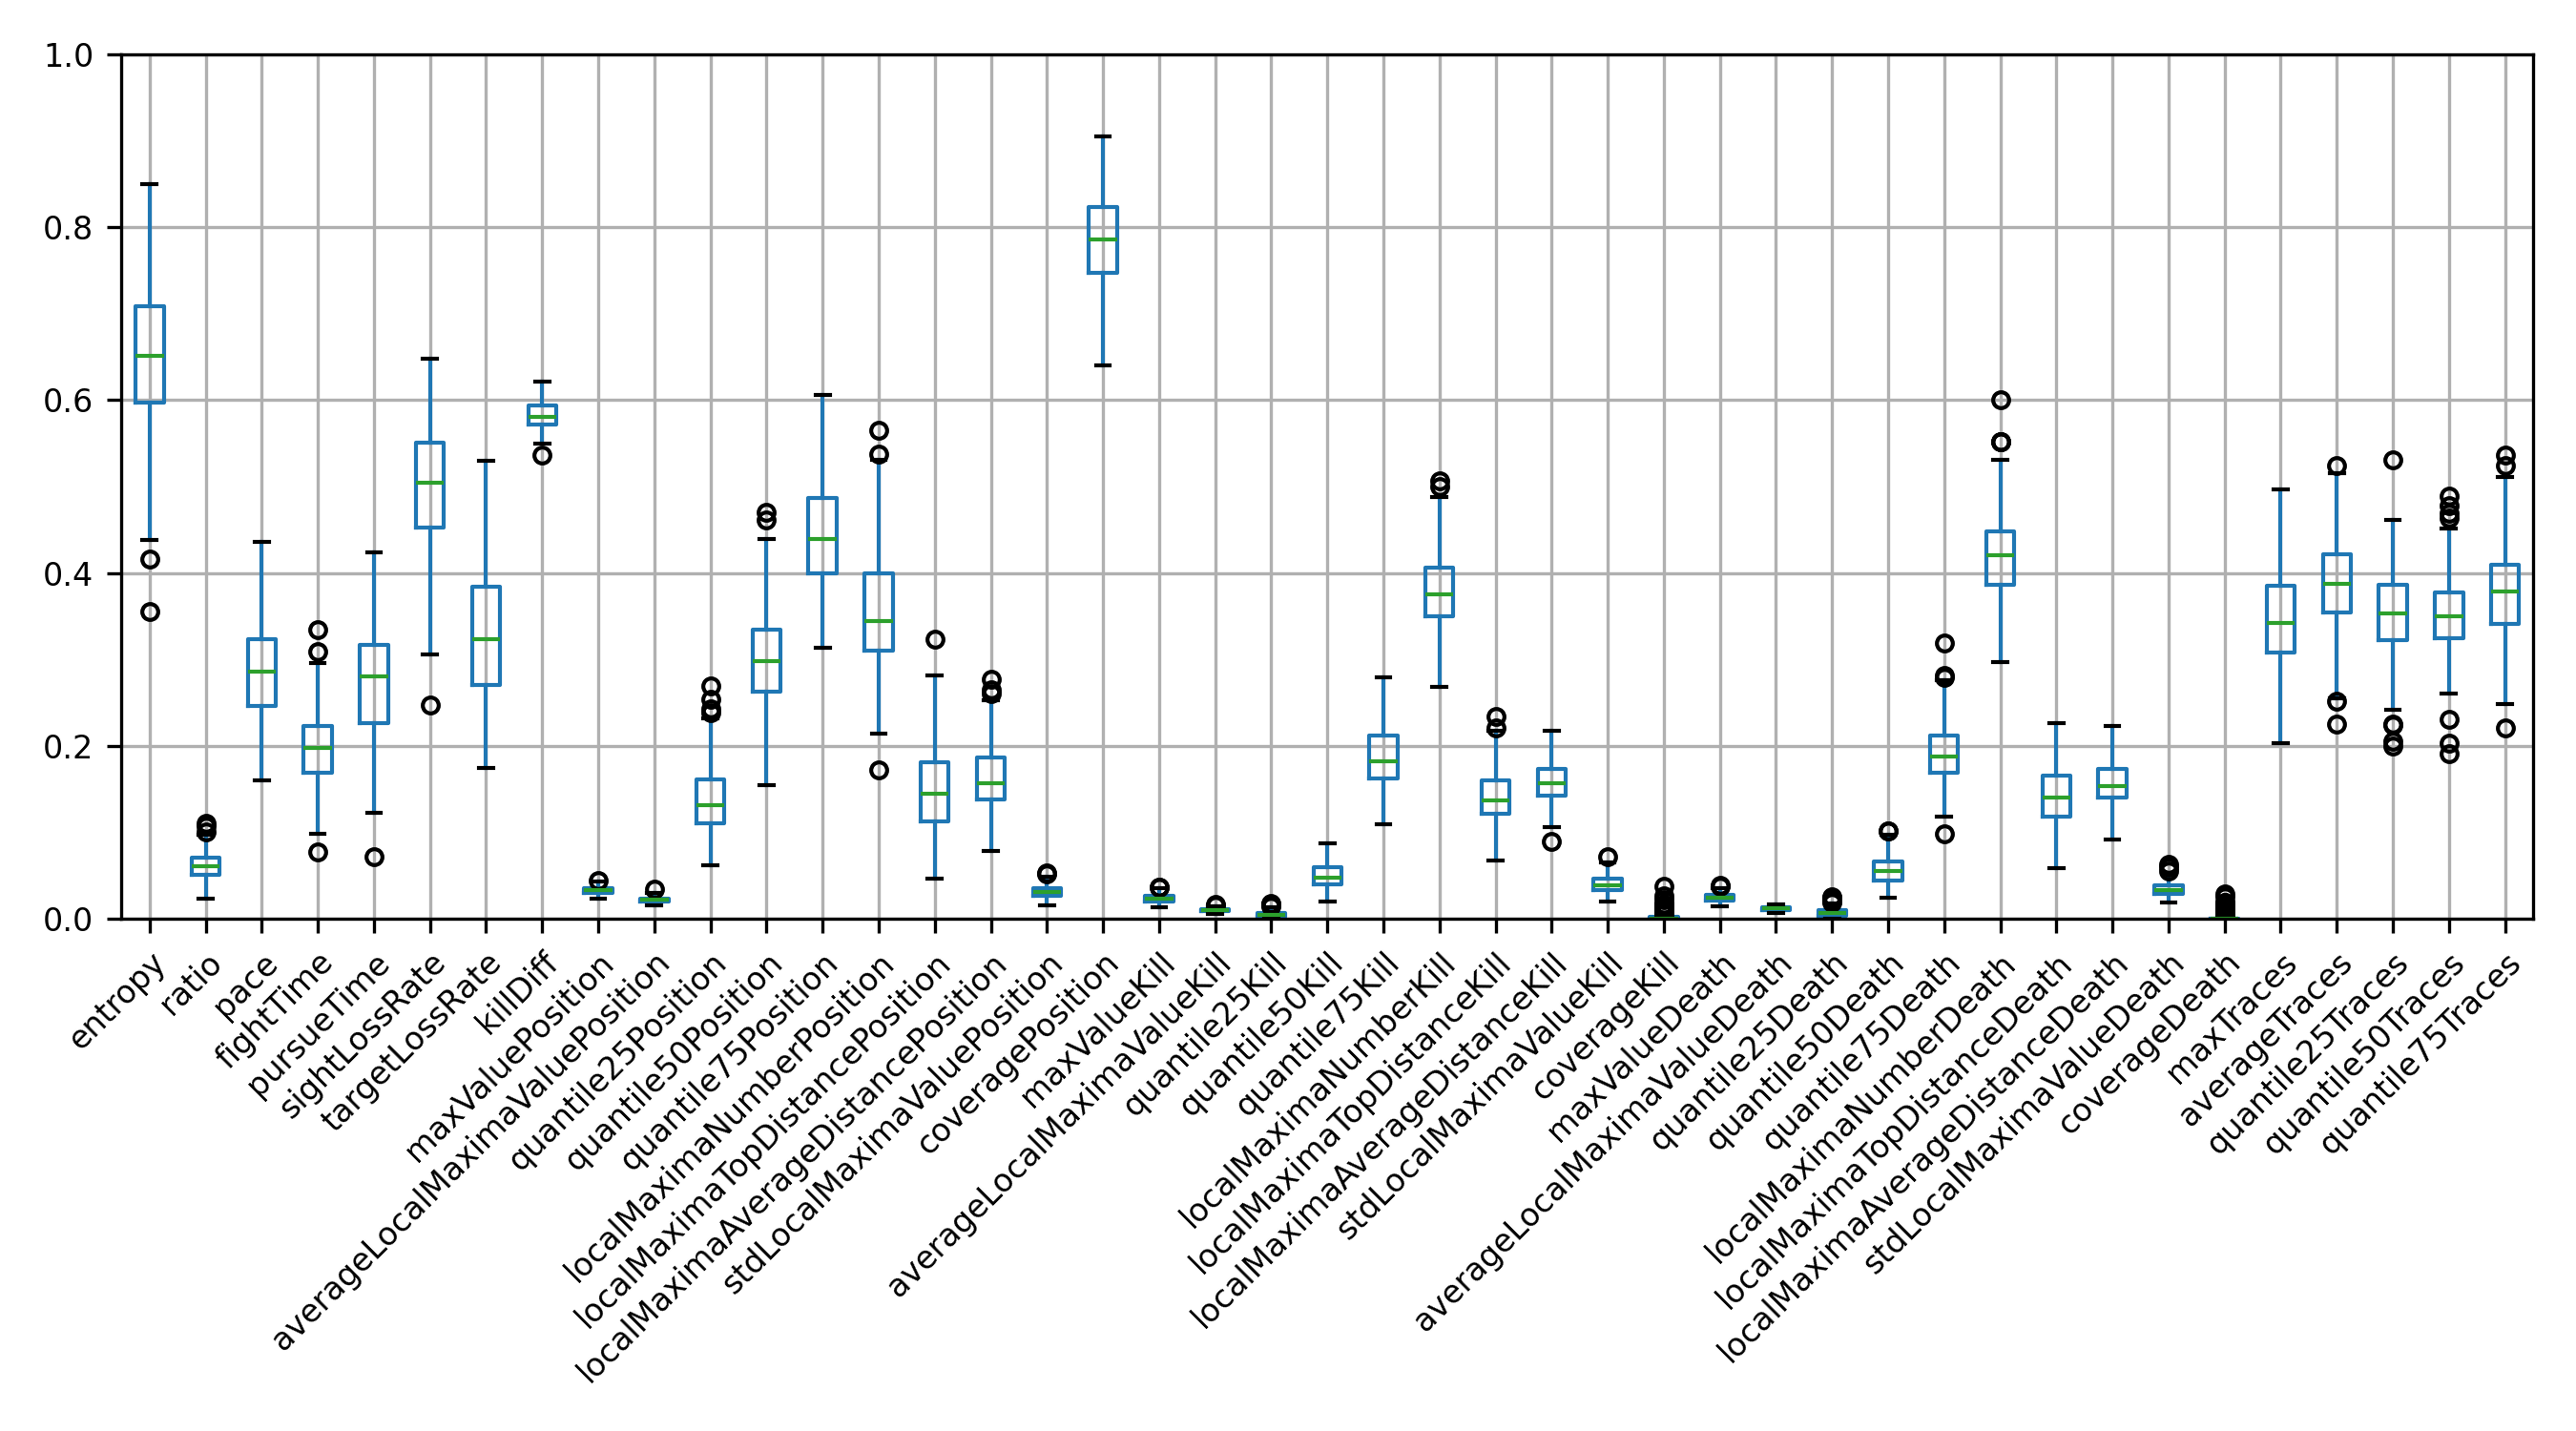
\includegraphics[width=0.85\textwidth]{images/boxplot_emergent_smtnoise_f_run2_numsim_5.png}
        }
    \caption{SMT-Genome emergent features noisiness analysis.}
    \label{fig:smt_genome_noisiness_emergent}
\end{figure}
\begin{figure}[hbt!]
    \centering
    \subfloat{
        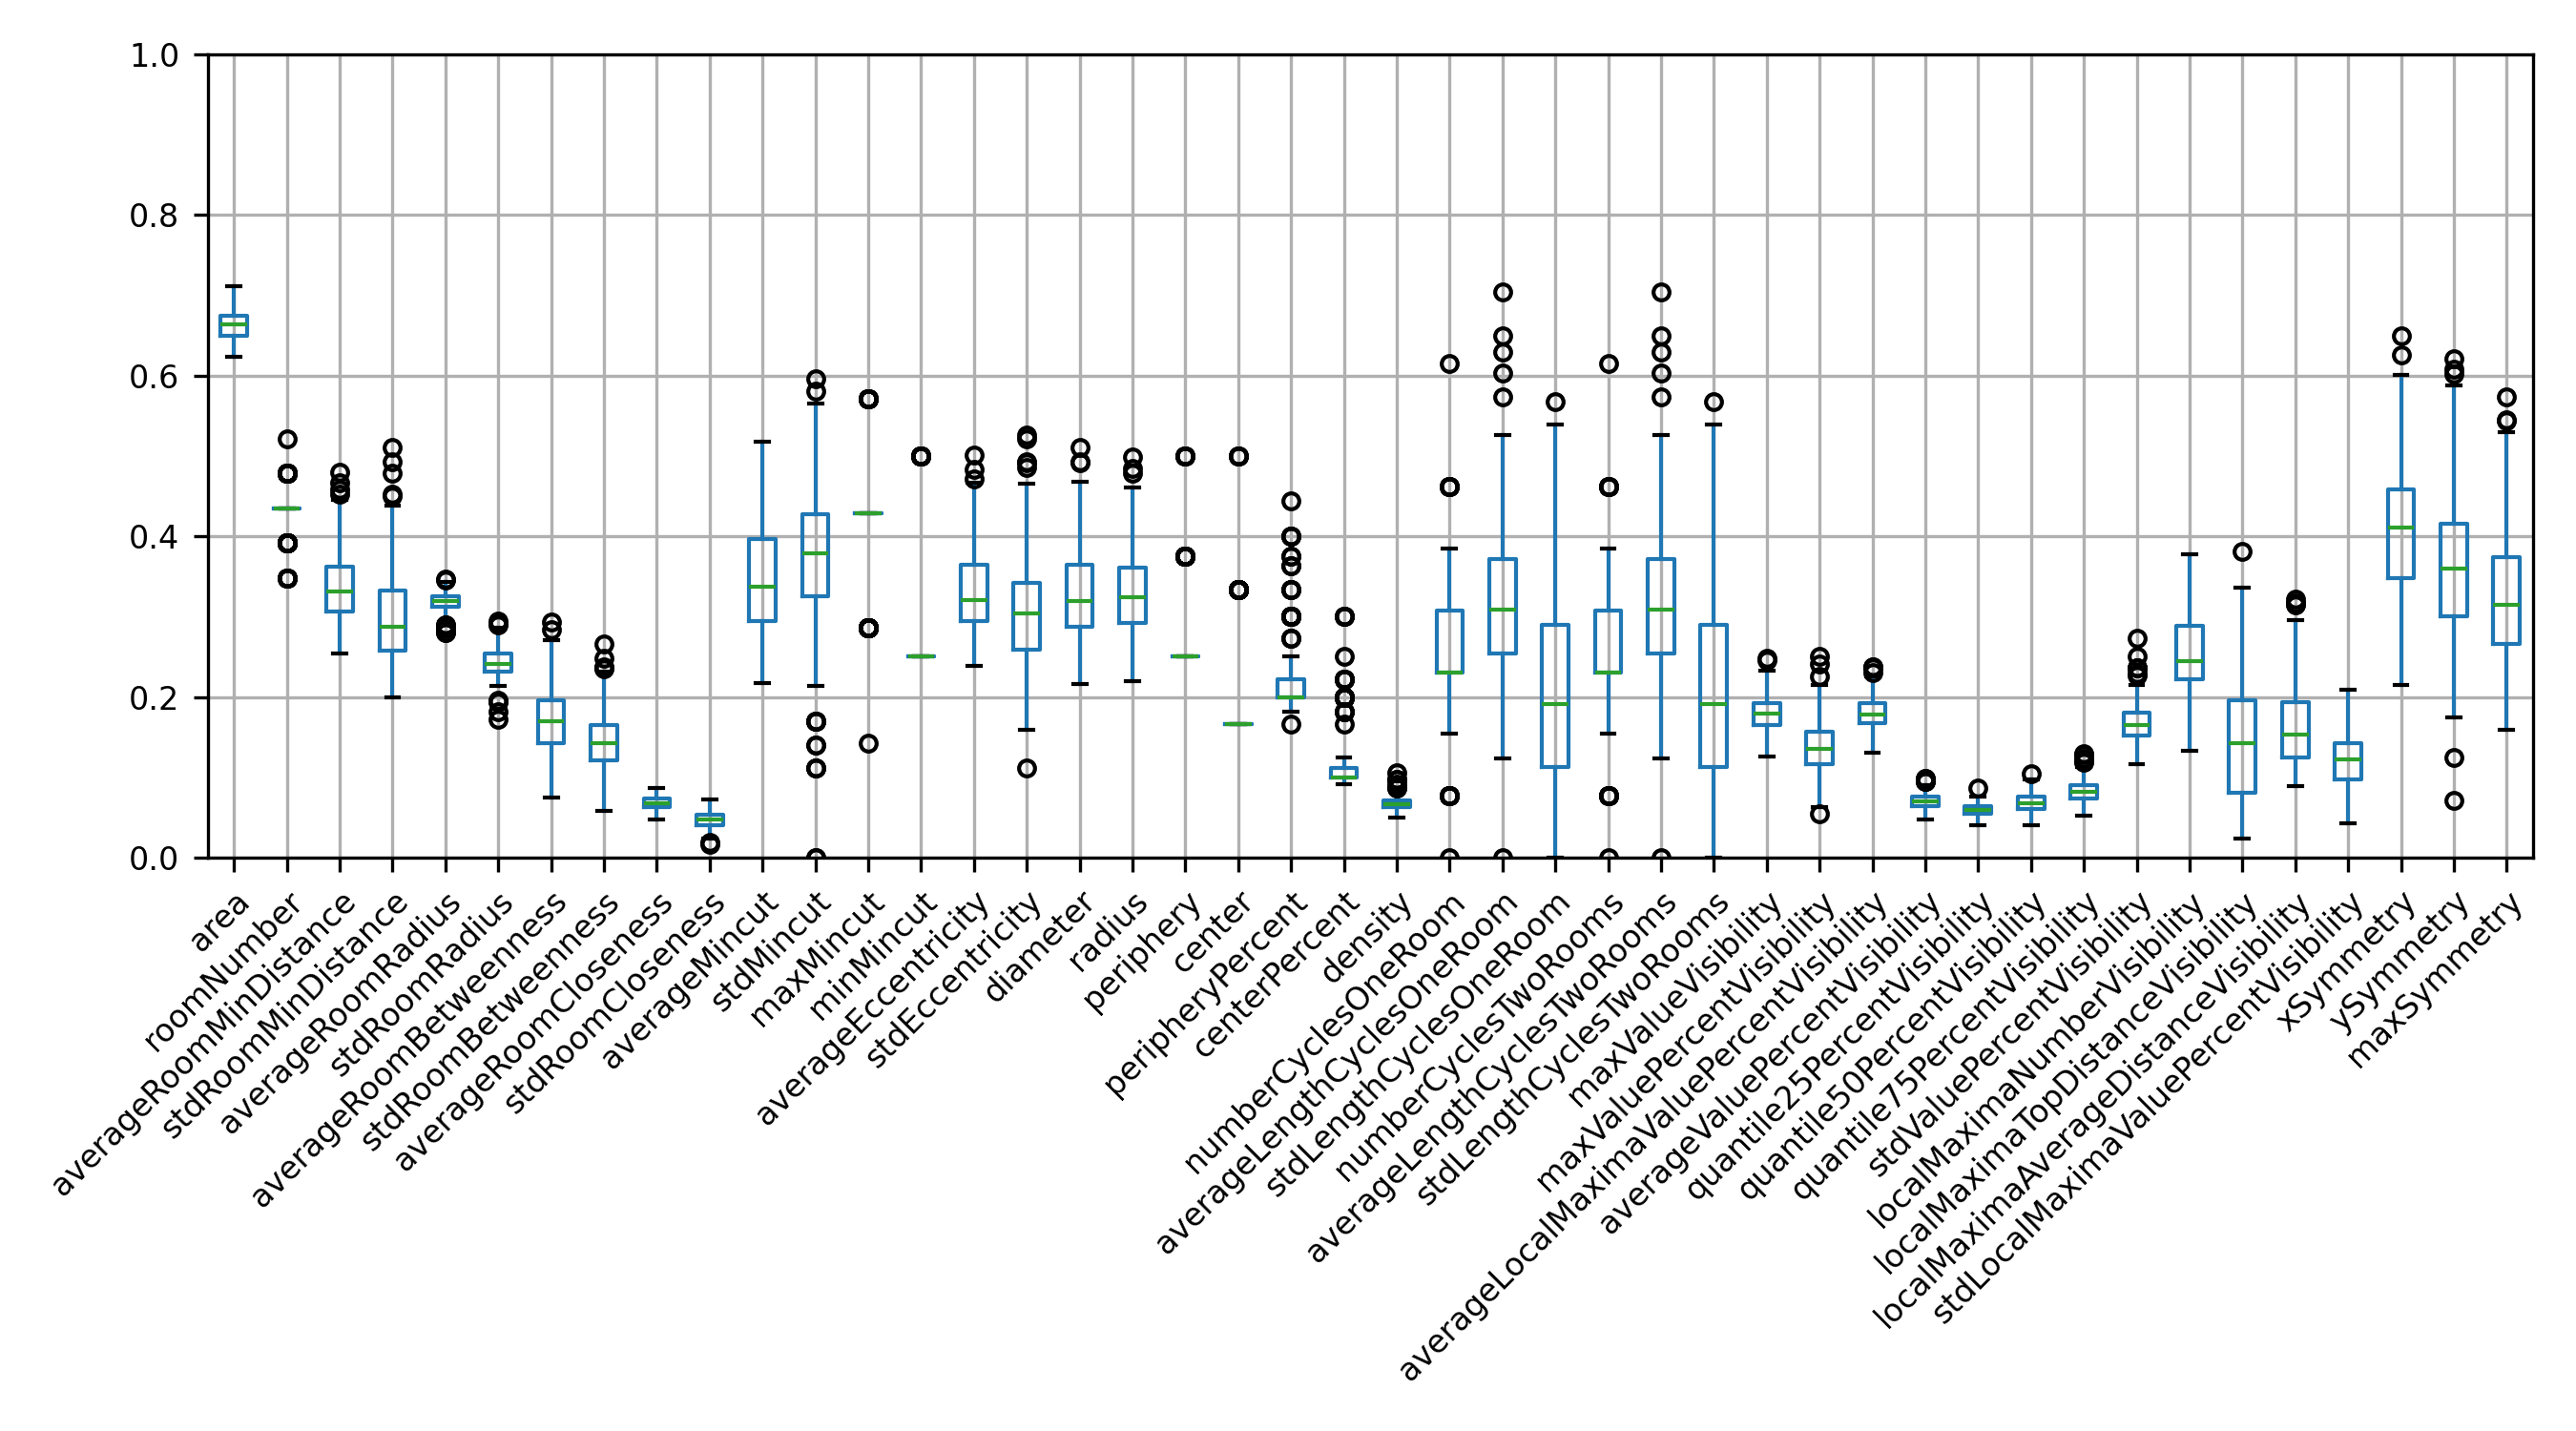
\includegraphics[width=0.85\textwidth]{images/boxplot_topology_smtnoise_f_run2_numsim_5.png}
    }
    \caption{SMT-Genome topological features noisiness analysis.}
    \label{fig:smt_genome_noisiness_topology}
\end{figure}

For the emergent features in figure \cref{fig:smt_genome_noisiness_emergent} we can clearly see that some features are very noisy, such as entropy, pace, sightLossRate and targetLossRate. For the topological features in figure \cref{fig:smt_genome_noisiness_topology} we can see that the features relating to the cycles are especially noisy, this is probably a consequence of the process of adding connections between rooms based on the lines in the genome, as described in \cref{subsec:smt_genome}, which relies on the intersection between lines and rooms, so often moving the room by a single tile can lead to the room not intersecting a line and thus to a completely different graph. This leads us to believe that the \textit{SMT-Genome} sports very little locality which may impact the evolution process negatively.

\section{Correlation analysis}
\label{sec:correlation_analysis}
Given the considerable number of features that can be extracted from a single map, it would be unfeasible to  try and illuminate all of them. Instead, we examined the correlations of the features with the aim of discovering relevant groups of highly correlated features, which could serve as a basis to explore with a QD method. Knowing how features correlate with one another will give us insights in how exploring a certain feature may affect others and will also help us in exploring interesting areas of the feature space by illuminating couples of features which are negatively correlated.

We generated 100 random genomes and simulated 5 matches on each map, averaging the features obtained in those matches. We used these 100 data points to compute the correlation matrix of the features using Pearson's correlation coefficient\footnote{Correlation coefficient which measures the linear correlation between two sets of data. Its value range from -1 (perfect negative correlation) to 1 (perfect positive correlation), with 0 indicating no correlation.}. We repeated this process for each of the four genome representations, obtaining one correlation matrix for each representation. In order to visualize the data more easily, we averaged the coefficients of these four matrices, obtaining the correlation matrix shown in figure \cref{fig:correlation_matrix_full}.

\begin{figure}[hbt!]
    \centering
    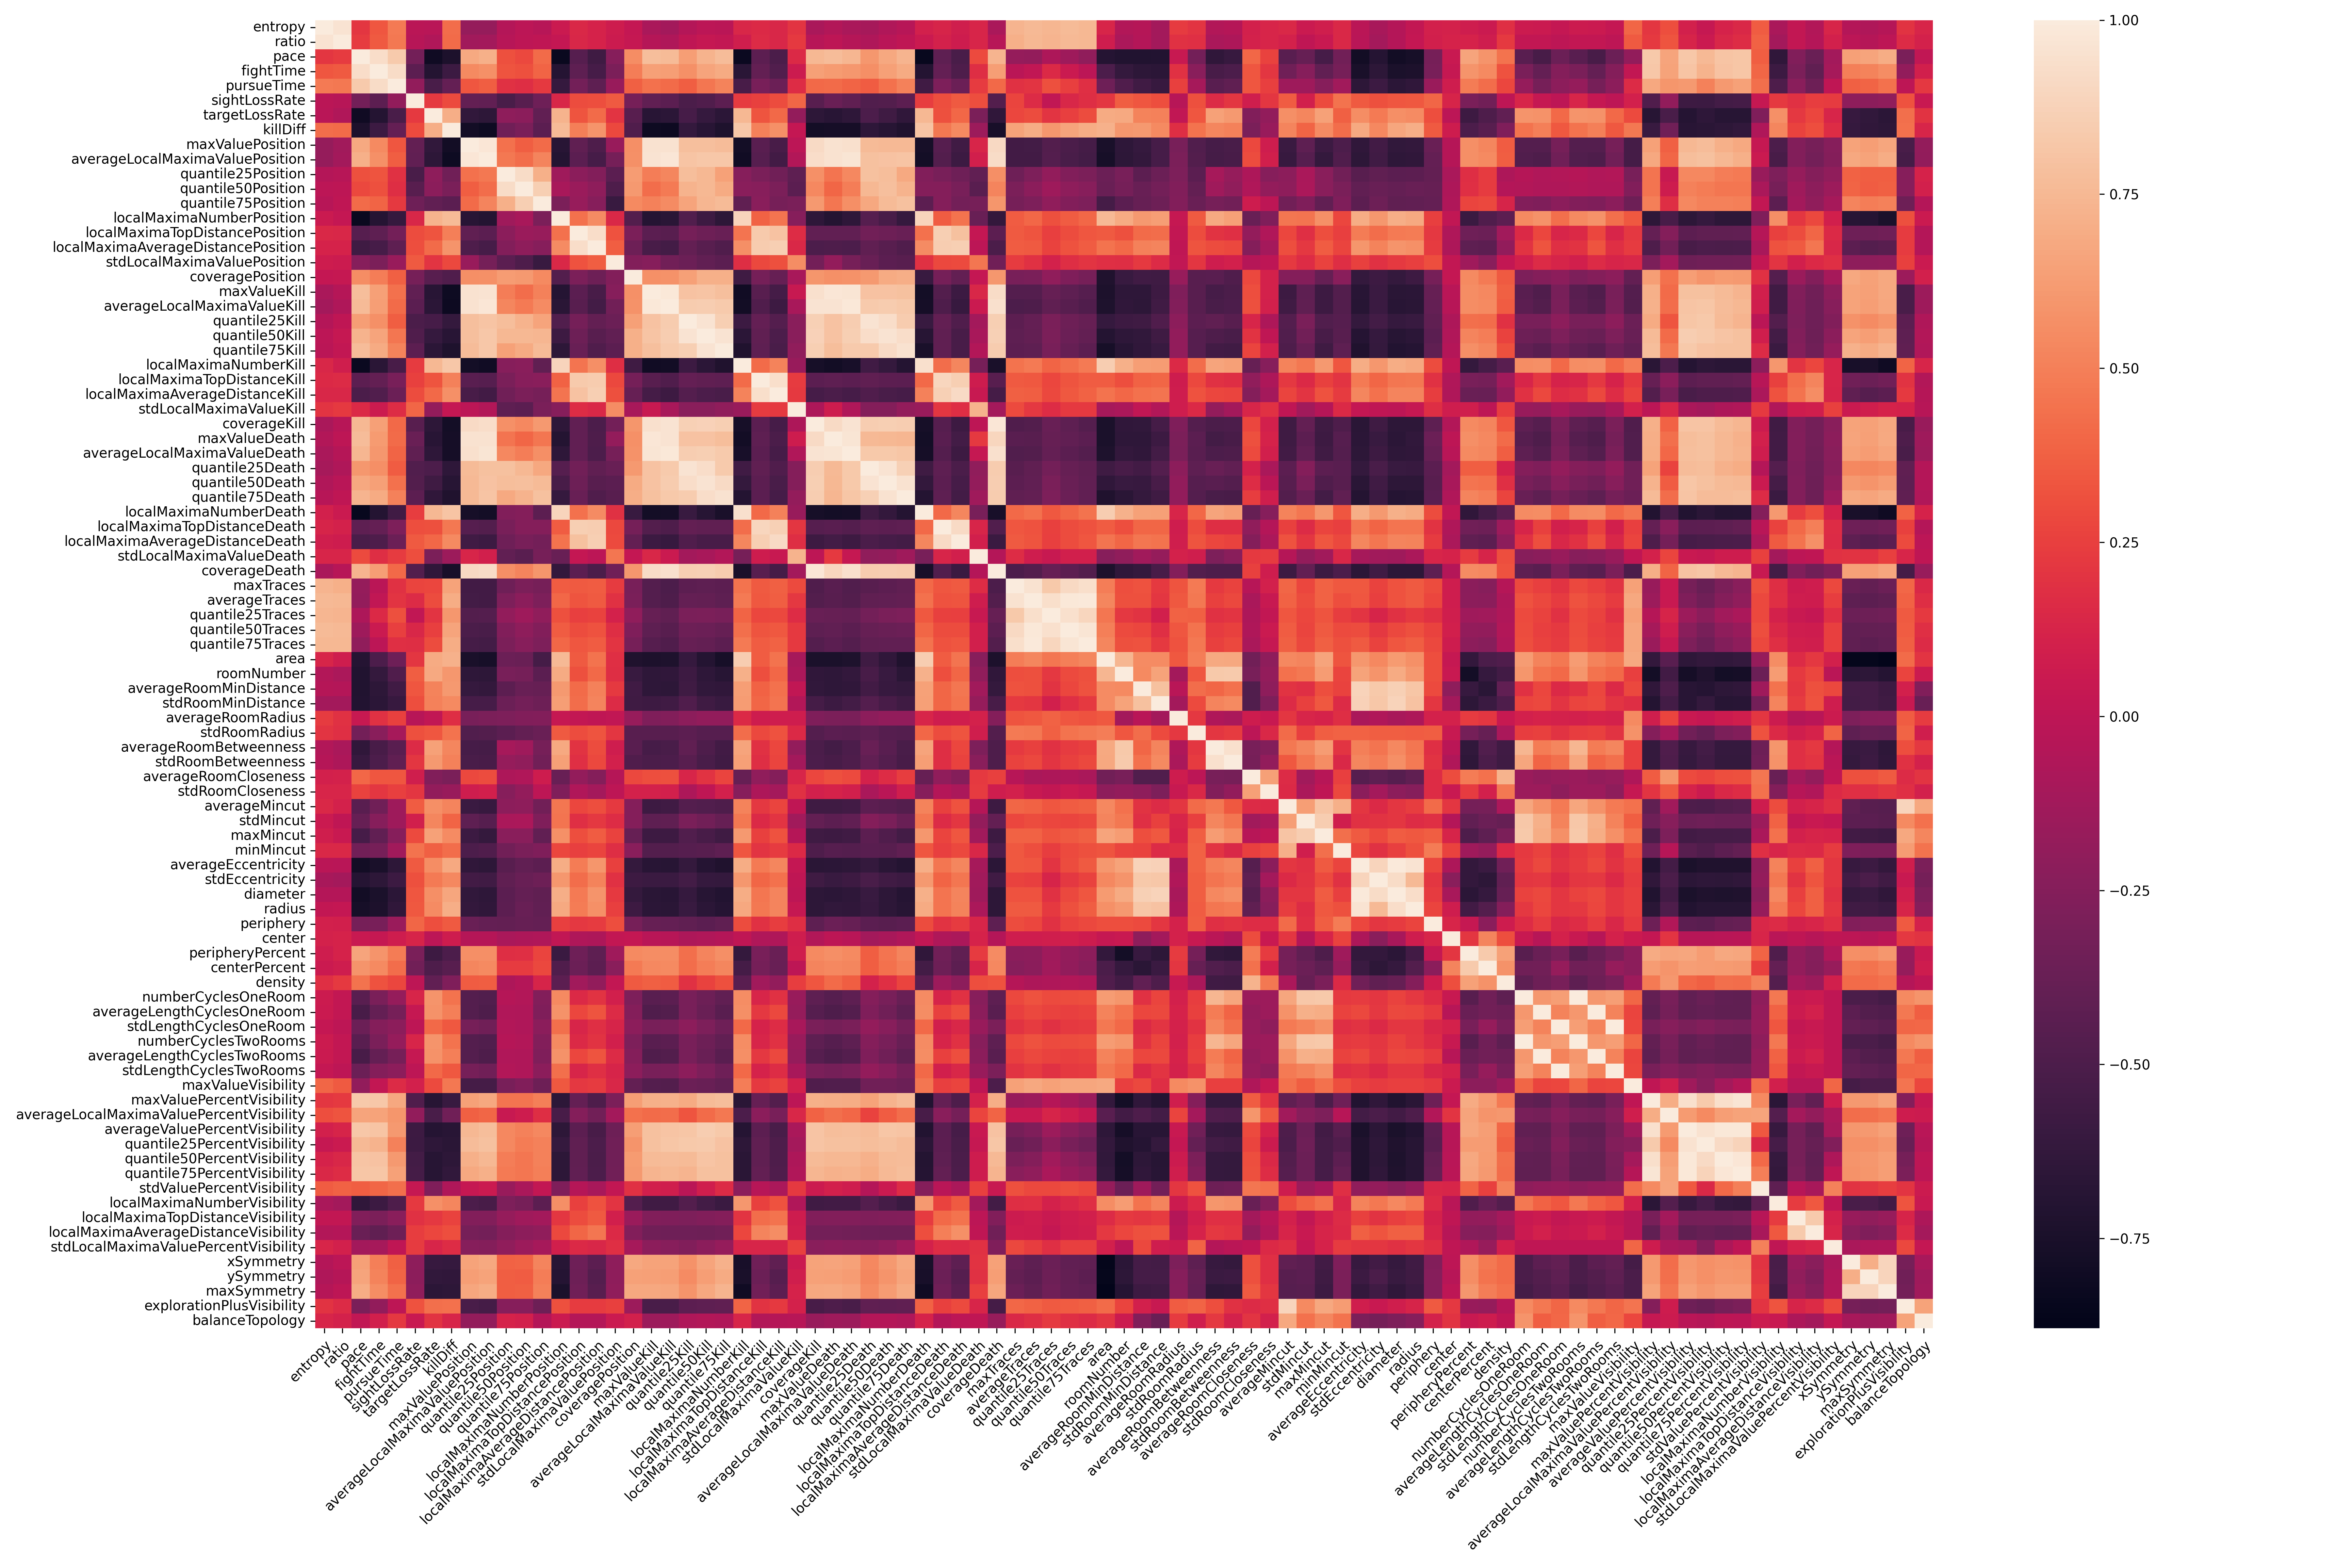
\includegraphics[width=1.0\textwidth]{images/covariance_map_full.png}
    \caption{Correlation matrix of the features.}
    \label{fig:correlation_matrix_full}
\end{figure}

It is immediately apparent that multiple features are not only highly correlated, as highlighted by the white squares on the diagonal, but also that they have similar correlation values with all other features, since multiple consecutive rows show similar values for all cells. Features are ordered on the axis "semantically", meaning that features that are conceptually similar are close to each other. Thus, we first group features by selecting only one feature from each group of highly correlated features (e.g. we select \textit{pace} between the similar \textit{pace}, \textit{fightTime} and \textit{pursueTime}). We then repeated the correlation analysis on the reduced set of features, this time utilizing a clustermap\footnote{\url{https://seaborn.pydata.org/generated/seaborn.clustermap.html}} to better visualize the remaining correlation between features that may not be conceptually similar, as seen in figure \cref{fig:correlation_clustermap_reduced}.

\begin{figure}[hbt!]
    \centering
    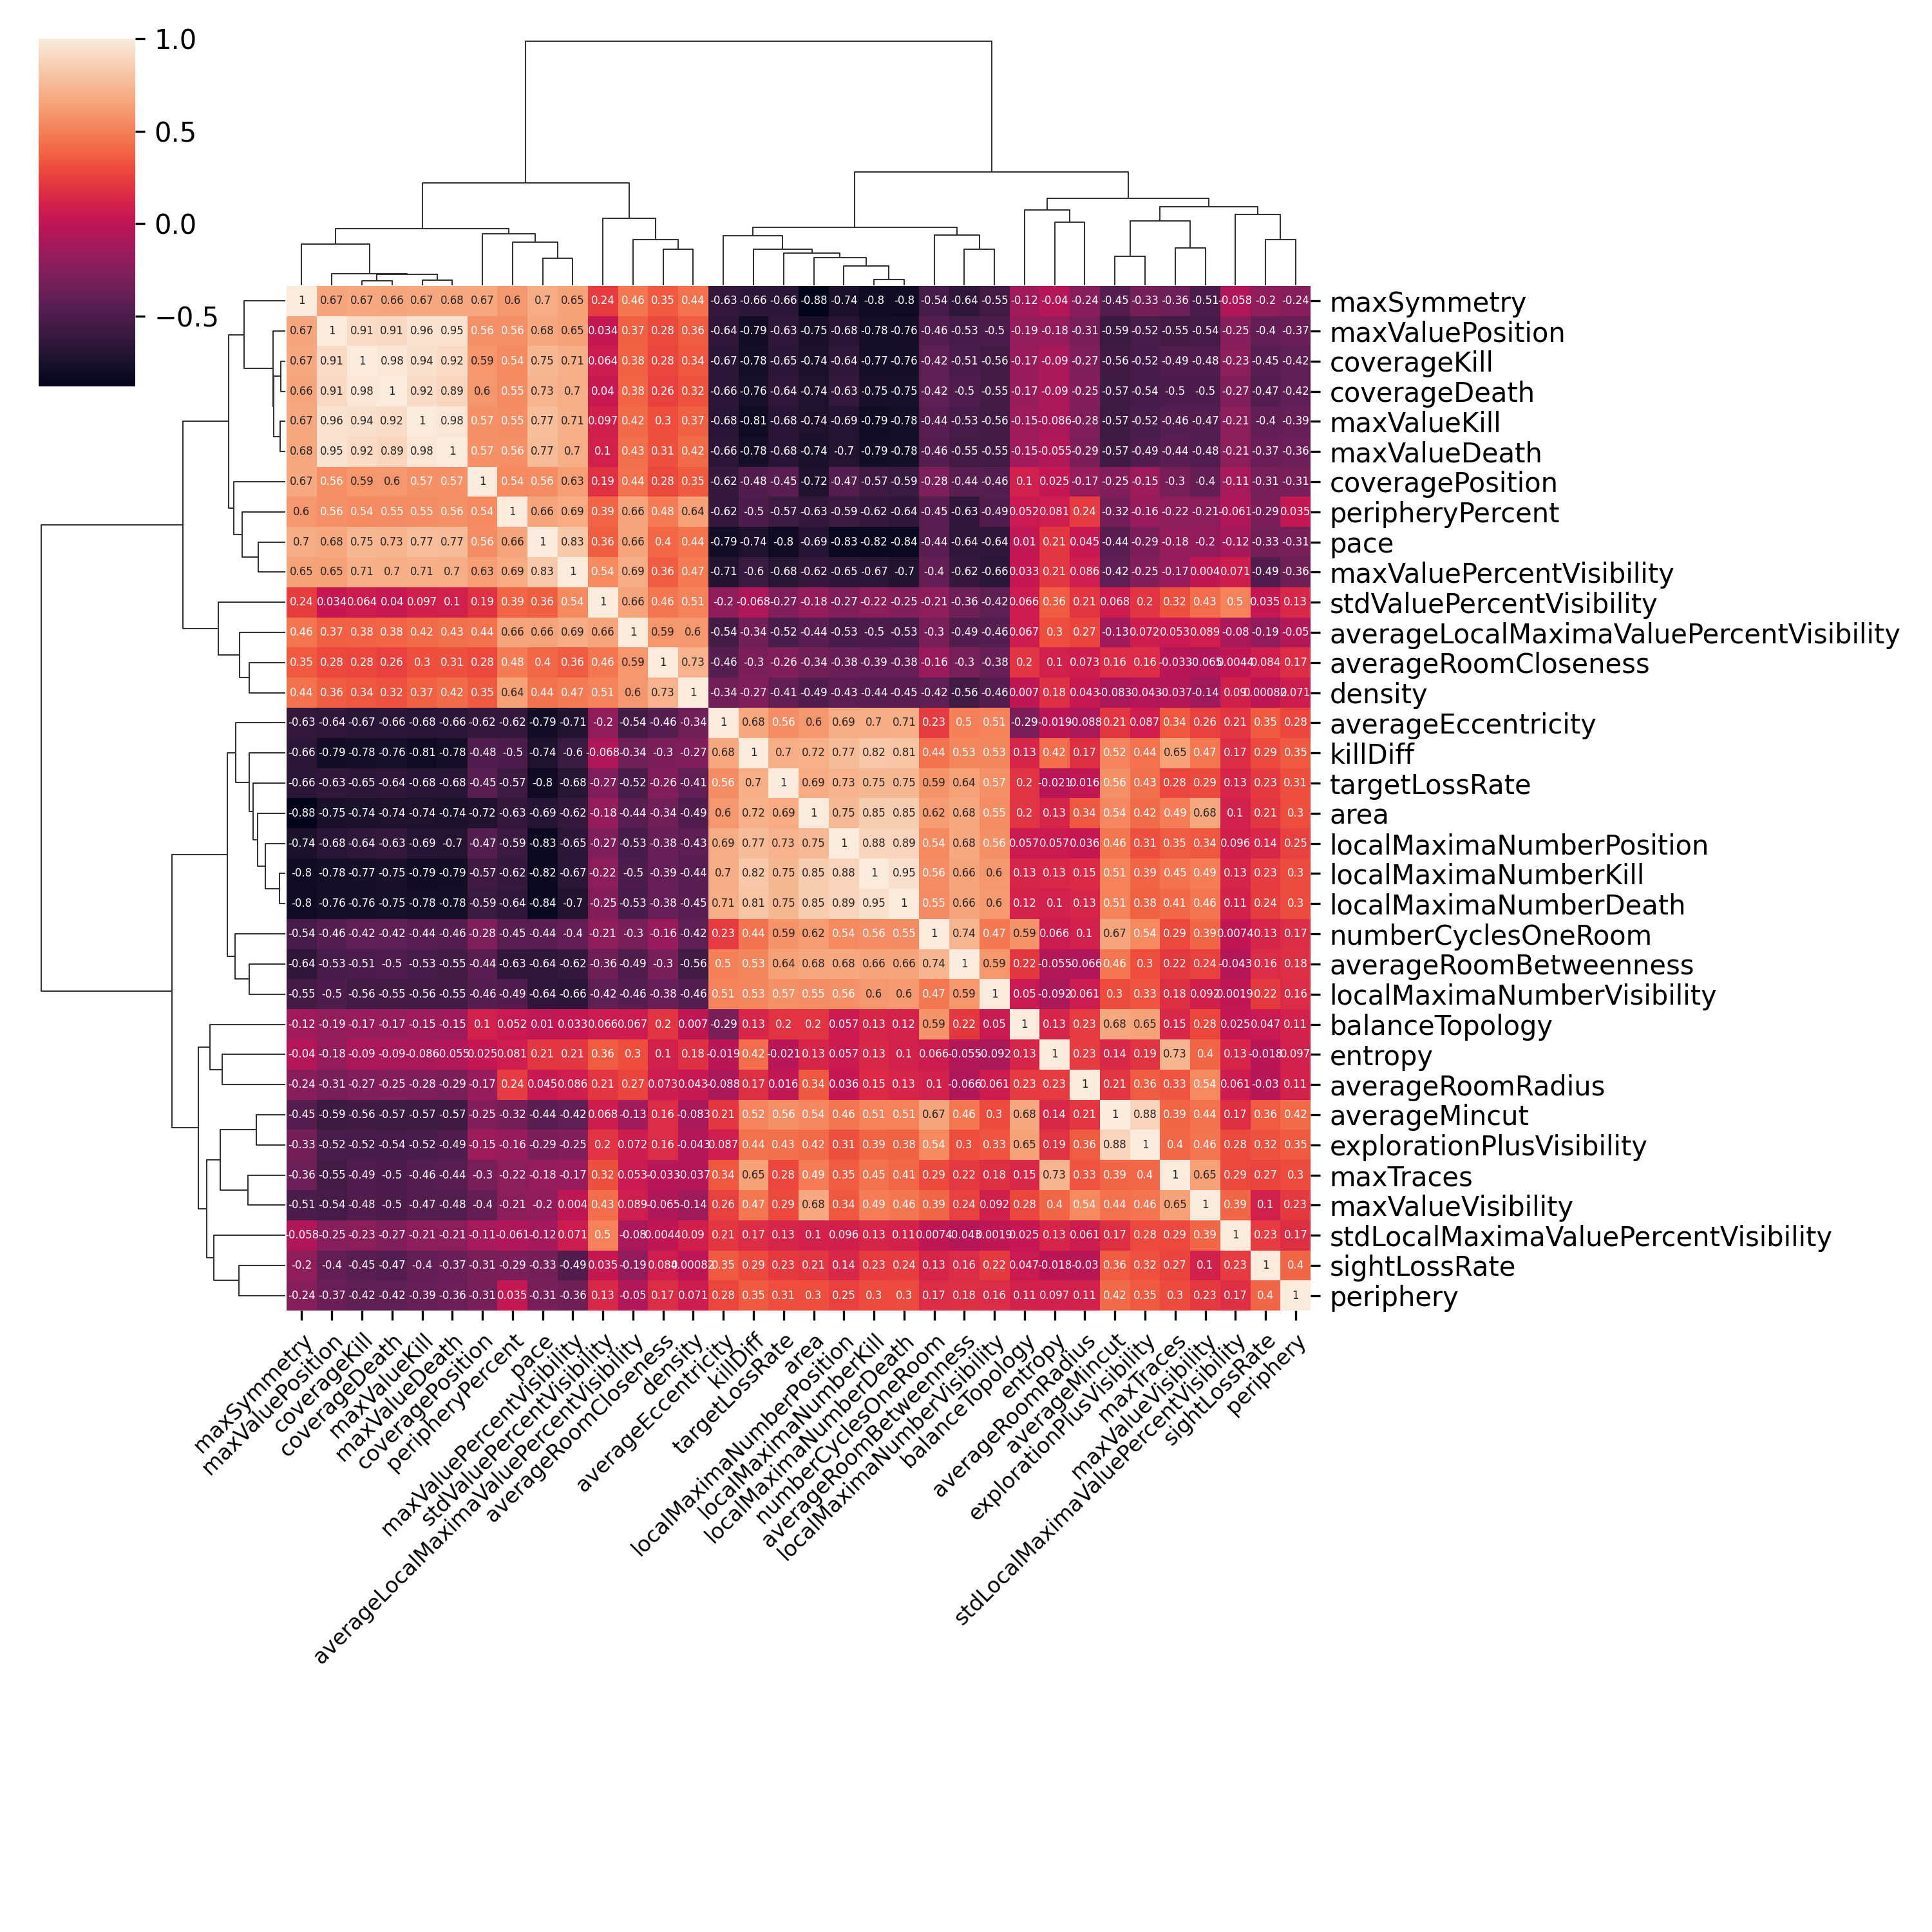
\includegraphics[width=1.0\textwidth]{images/covariance_clustermap_reduced.png}
    \caption{Clustermap of the reduced set of features.}
    \label{fig:correlation_clustermap_reduced}
\end{figure}

The clustering helps us observe varied groups of features that are still highly correlated. To improve the grouping and to further reduce the number of features to examine, we selected one feature from each highly correlated group, preferring features that are conceptually more interesting. We consider features highly correlated when their correlation coefficient is greater than 0.7. 

In summary, we get the following final list of features, along with the resulting group, from this two-step process:

\begin{itemize}
    \item \textbf{\textit{maxSymmetry}} (grouped with \textit{xSymmetry}, \textit{ySymmetry})
    \item \textbf{\textit{maxValuePosition}} (grouped with \textit{averageLocalMaximaValuePosition}, \textit{quantile25\-Position}, \textit{quantile50\-Position}, \textit{quantile75\-Position}, \textit{coverageKill}, \textit{coverageDeath}, \textit{maxValueKill}, \textit{averageLocalMaximaValueKill}, \textit{quantile25\-Kill}, \textit{quantile50\-Kill}, \textit{quantile75\-Kill}, \textit{maxValueDeath}, \textit{averageLocalMaximaValueDeath}, \textit{quantile25\-Death}, \textit{quantile50\-Death}, \textit{quantile75\-Death})
    \item \textbf{\textit{coveragePosition}}
    \item \textbf{\textit{peripheryPercent}} (grouped with \textit{centerPercent})
    \item \textbf{\textit{pace}} (grouped with \textit{fightTime}, \textit{pursueTime}, \textit{maxValuePercentVisibility})
    \item \textbf{\textit{stdValuePercentVisibility}} 
    \item \textbf{\textit{averageLocalMaximaValuePercentVisibility}} (grouped with \textit{averageValuePercentVisibility}, \textit{quantile25PercentVisibility}, \textit{quantile50PercentVisibility}, \textit{quantile75\-Percent\-Visibility})
    \item \textbf{\textit{density}} (grouped with \textit{averageRoomCloseness}, \textit{stdRoomCloseness})
    \item \textbf{\textit{averageEccentricity}} (grouped with \textit{stdEccentricity}, \textit{diameter}, \textit{radius})
    \item \textbf{\textit{area}} (grouped with \textit{killDiff}, \textit{targetLossRate}, \textit{localMaximaNumberPosition}, \textit{localMaximaTopDistancePosition}, \textit{localMaximaAverageDistancePosition}, \textit{stdLocalMaximaValuePosition}, \textit{localMaximaNumberKill}, \textit{localMaximaTopDistanceKill}, \textit{localMaximaAverageDistanceKill}, \textit{stdLocalMaxima\-Value\-Kill}, \textit{localMaximaNumberDeath}, \textit{localMaximaTopDistanceDeath}, \textit{localMaximaAverageDistanceDeath}, \textit{stdLocalMaxima\-Value\-Death})
    \item \textbf{\textit{averageRoomBetweenness}} (grouped with \textit{stdRoomBetweenness})
    \item \textbf{\textit{localMaximaNumberVisibility}} (grouped with \textit{localMaximaTopDistanceVisibility}, \textit{localMaximaAverageDistanceVisibility})
    \item \textbf{\textit{balanceTopology}}
    \item \textbf{\textit{entropy}} (grouped with \textit{ratio})
    \item \textbf{\textit{averageRoomRadius}} (grouped with \textit{stdRoomRadius})
    \item \textbf{\textit{stdLocalMaximaValuePercentVisibility}}
    \item \textbf{\textit{sightLossRate}}
    \item \textbf{\textit{periphery}} (grouped with \textit{center})
    \item \textbf{\textit{maxTraces}} (grouped with \textit{averageTraces}, \textit{quantile25Traces}, \textit{quantile50Traces}, \textit{quantile75Traces})
    \item \textbf{\textit{maxValueVisibility}}
    \item \textbf{\textit{numberCyclesOneRoom}} (grouped with \textit{averageLengthCyclesOneRoom}, \textit{stdLengthCyclesOneRoom}, \textit{numberCyclesTwoRooms}, \textit{averageLengthCyclesTwoRooms}, \textit{stdLengthCyclesTwoRooms})
    \item \textbf{\textit{averageMincut}} (grouped with \textit{stdMincut}, \textit{maxMincut}, \textit{minMincut}, \textit{explorationPlusVisibility})
\end{itemize}

Finally, in figure \cref{fig:correlation_clustermap_final} we show the correlation clustermap of the final set of features.

\begin{figure}[hbt!]
    \centering
    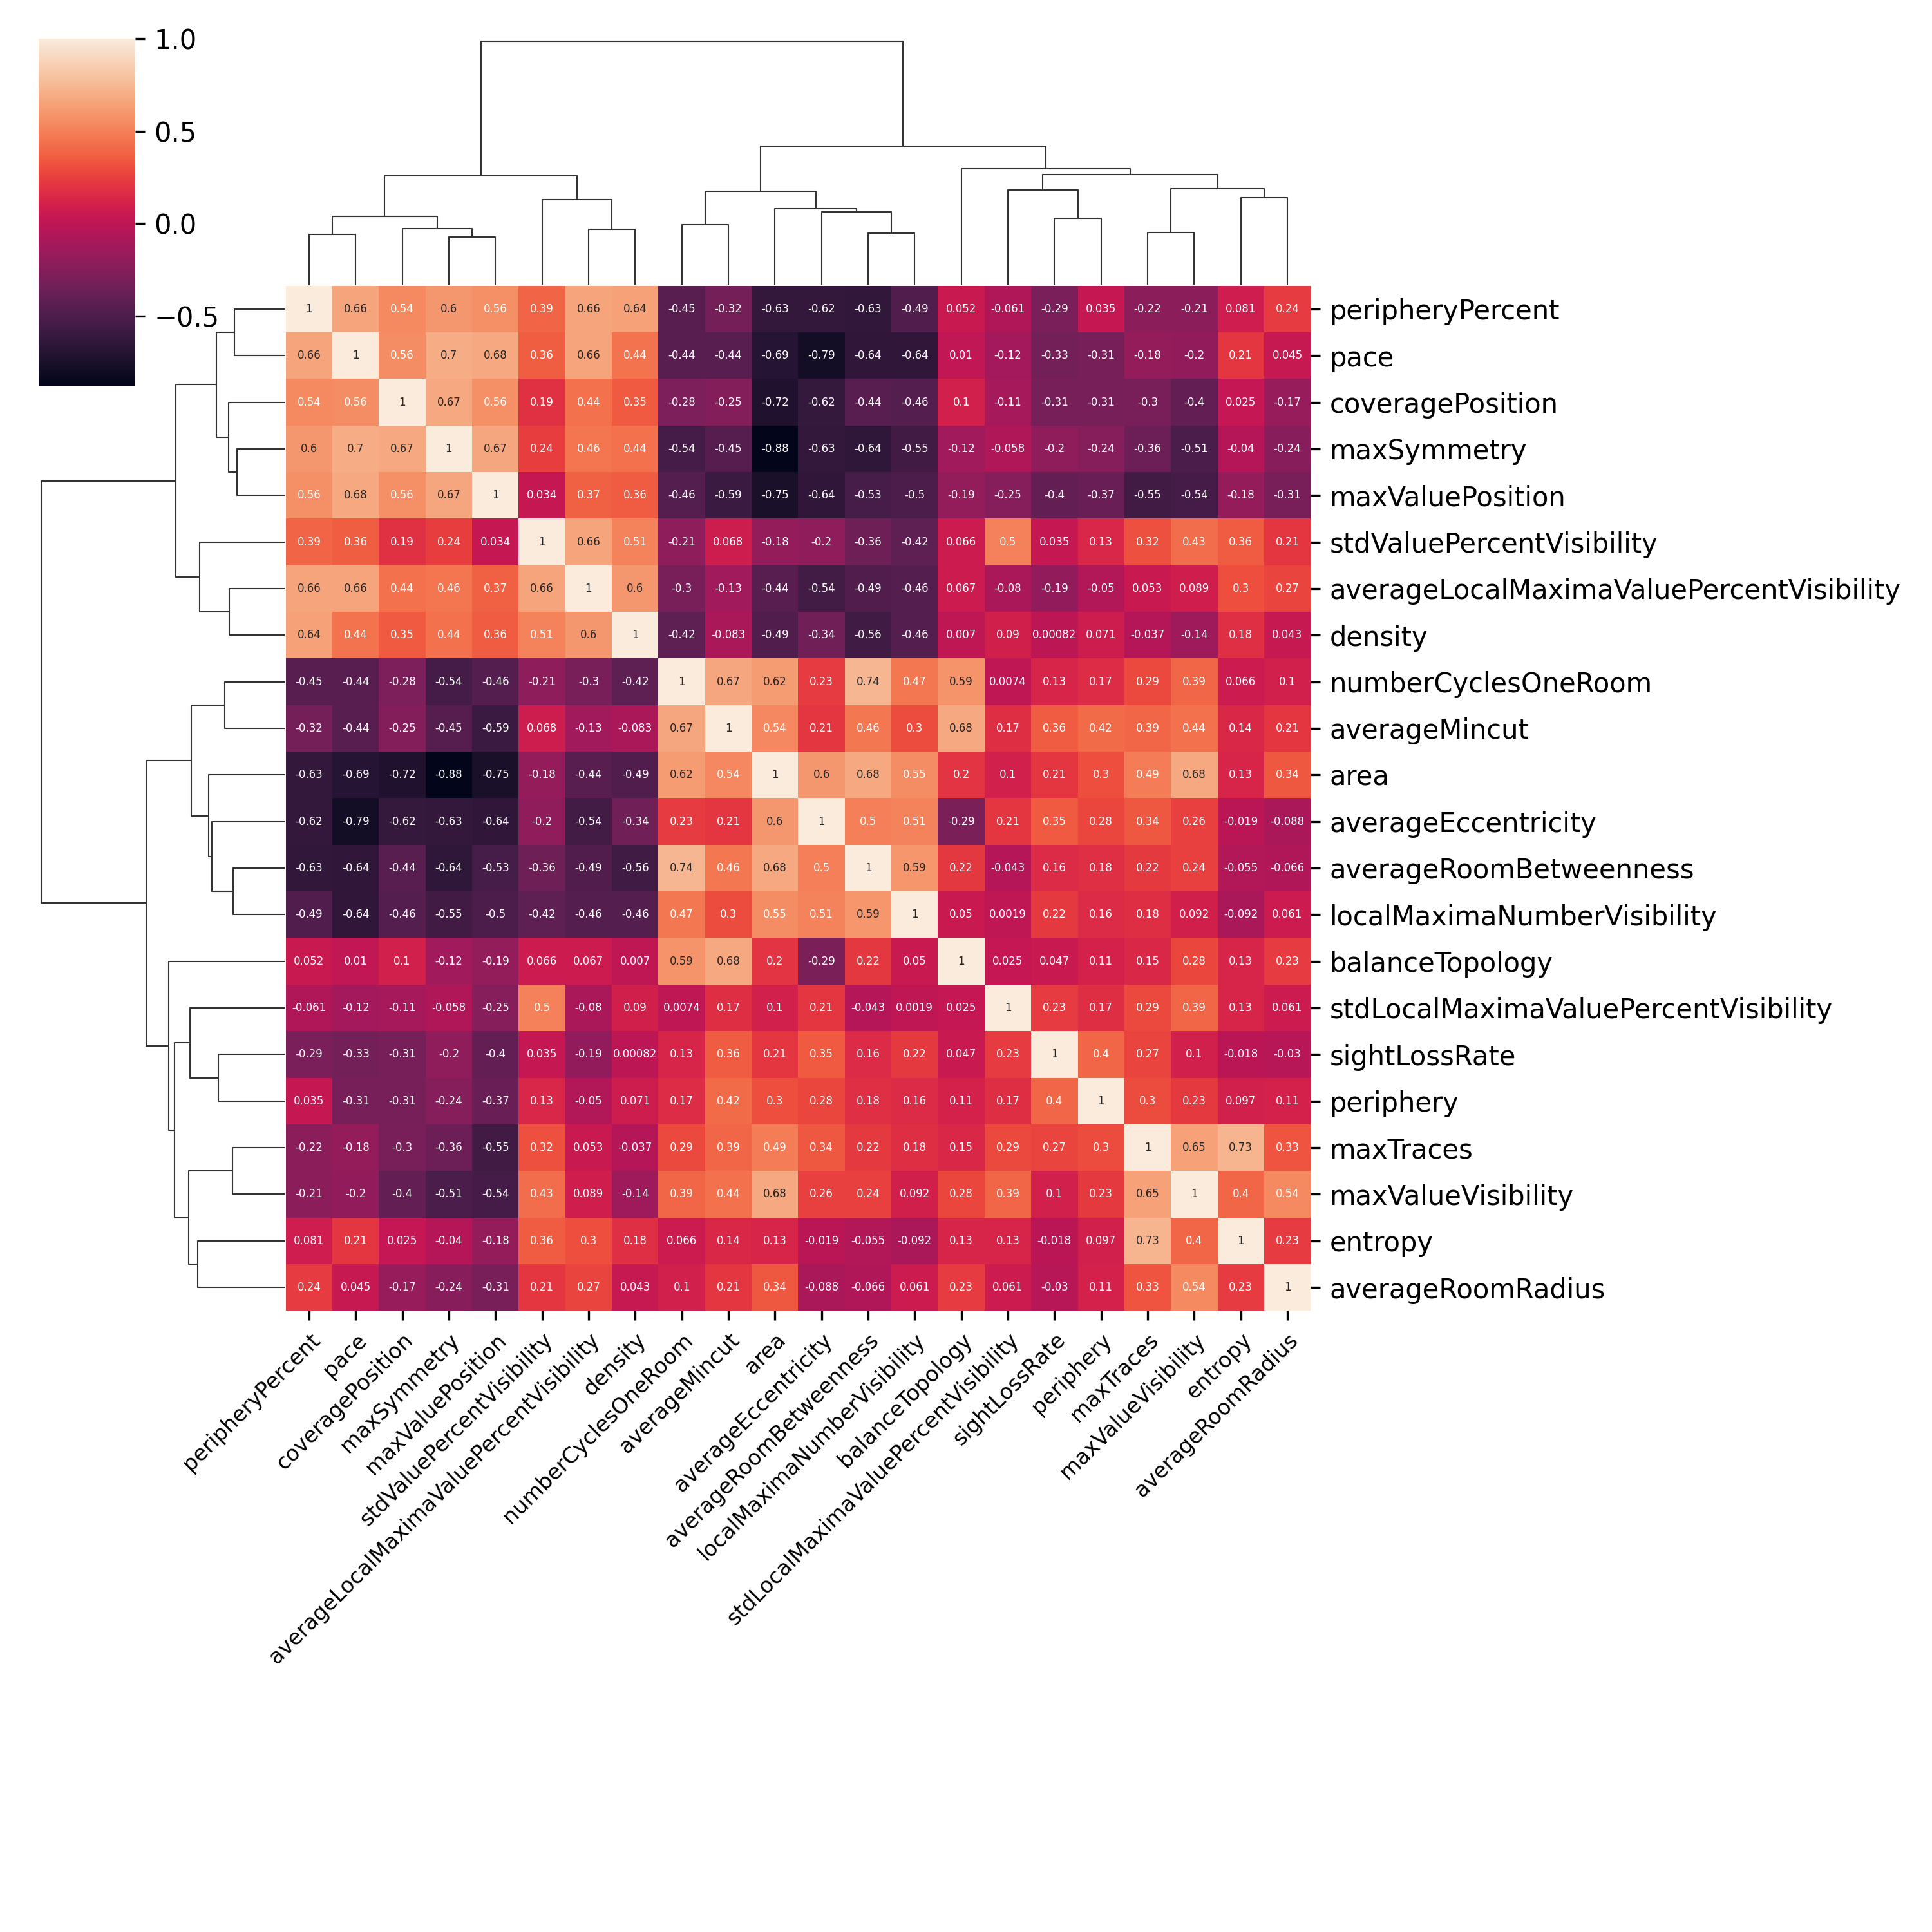
\includegraphics[width=1.0\textwidth]{images/covariance_clustermap_final.png}
    \caption{Clustermap of the final set of features.}
    \label{fig:correlation_clustermap_final}
\end{figure}

From this graph we are interested in observing couples of features that are strongly correlated negatively; these offer interesting potential to be illuminated using QD approaches, such as \textit{MAP-Elites}, as these kinds of approaches will try to explore fully the feature space. Illuminating, as an example, \textit{area} and \textit{maxSymmetry}, which are strongly correlated negatively, could allow us to find interesting designs, such as big maps that are symmetrical, that could remain otherwise unexplored, as they are statistically less probable to be generated. It will also allow us to compare representations to measure their capability to generate varied designs. 

We have thus identified the following interesting couples of features: 
\begin{itemize}
    \item \textit{area} / \textit{MaxSymmetry} (-0.88) 
    \item \textit{pace} / \textit{averageEccentricity} (-0.79) 
    \item \textit{averageMincut} / \textit{maxValuePosition} (-0.59)
    \item \textit{peripheryPercent} / \textit{averageRoomBetweennes} (-0.63)
    \item \textit{area} / \textit{coveragePosition} (-0.72)
    \item \textit{numberCyclesOneRoom}, \textit{maxSymmetry} (-0.54)
    \item \textit{maxTraces} / \textit{maxValuePosition} (-0.55) 
    \item \textit{maxValueVisibility} / \textit{maxValuePosition} (-0.54) 
    \item \textit{density} / \textit{averageRoomBetweennes} (-0.56).
\end{itemize}


\section{t-SNE analysis}
\label{sec:tsne_analysis}

\textit{t-SNE} is a state-of-the-art dimensionality reduction method, which is helpful to visualize high dimensional data in a projected 2D space. Points that are close in the original high-dimensional space will be placed close also in the space projected by \textit{t-SNE}; this allows clusters to form which can often be used to deduce and learn interesting properties of our data. 

For each representation we will employ a dataset consisting of 2000 maps and place each map in three different high-dimensional spaces (features, images and graphs) which we will visualize in a 2D space using \textit{t-SNE}, hoping to derive interesting insights about the correlation between the different spaces.

\subsection{t-SNE of the feature space}

We first used \textit{t-SNE} to reduce the feature space of the maps to 2 dimensions in order to plot each map as a point in a two-dimensional graph. Each point is assigned a color based on their position in the plot, according to a 4-way gradient. We ran the algorithm using a \textit{perplexity} value equal to 30. Fine-tuning this parameter can be troublesome when using t-SNE; in our case different perplexities (5, 10, 30, 50, 100) all led to comparable results. At this stage we are interested in visualizing the points' position in the two-dimensional space which will be useful later to understand how maps cluster based on their features. The results of this analysis are shown in figure \cref{fig:tsne_feature}.

\begin{figure}[hbt!]
    \centering
    \subfloat[All-black\label{fig:tsne_ab_feature}]{
        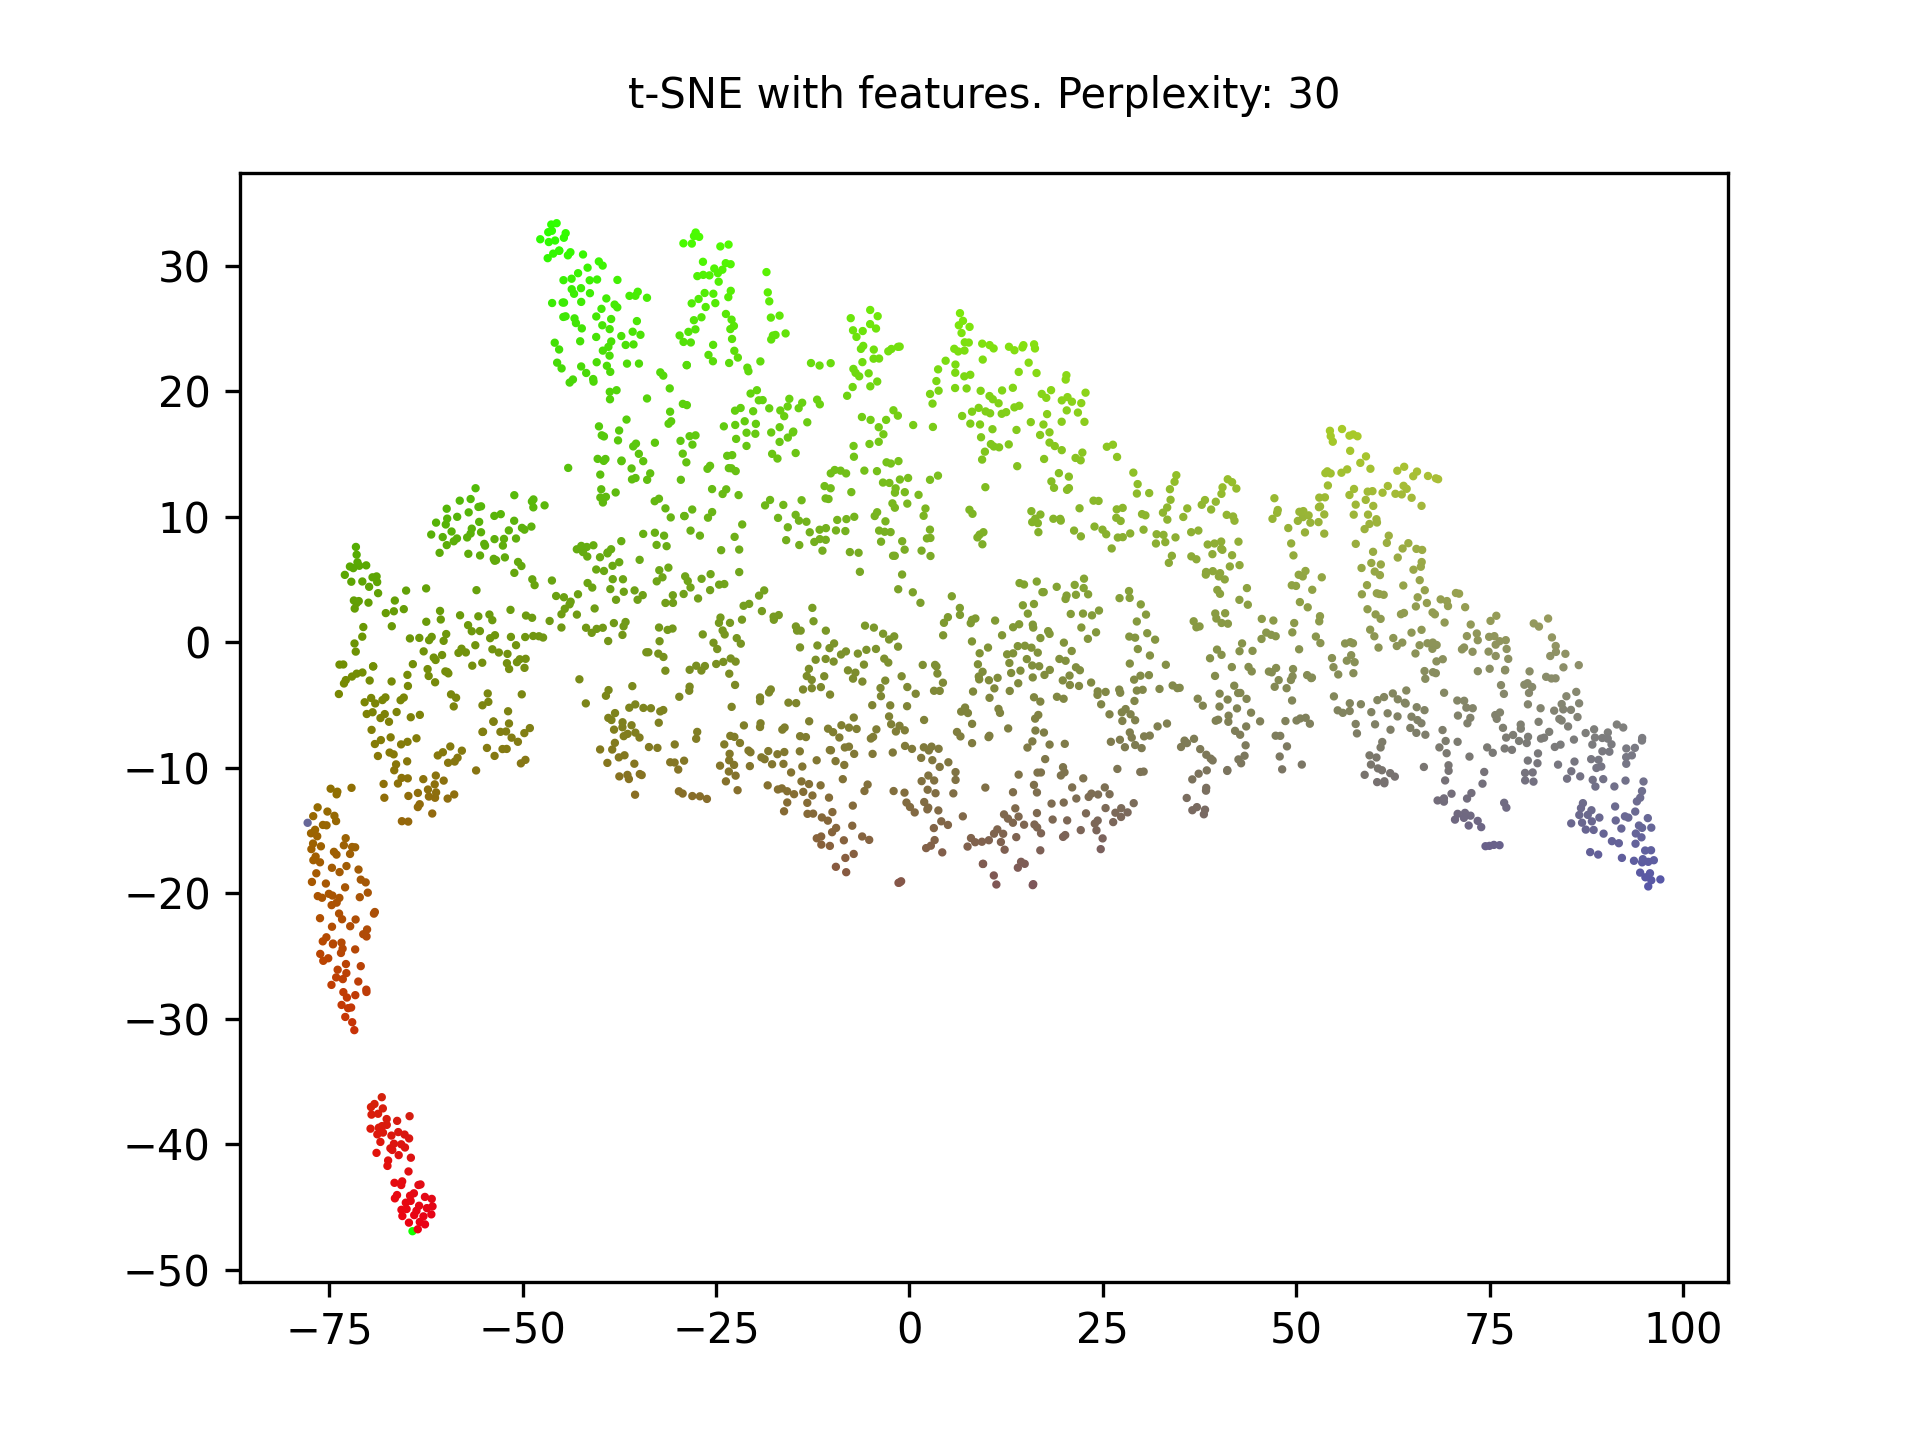
\includegraphics[width=0.45\textwidth]{images/tsne_ab_gl2vecAttr_features_p30.png}
    }
    \qquad
    \subfloat[Grid-Graph\label{fig:tsne_gg_feature}]{
        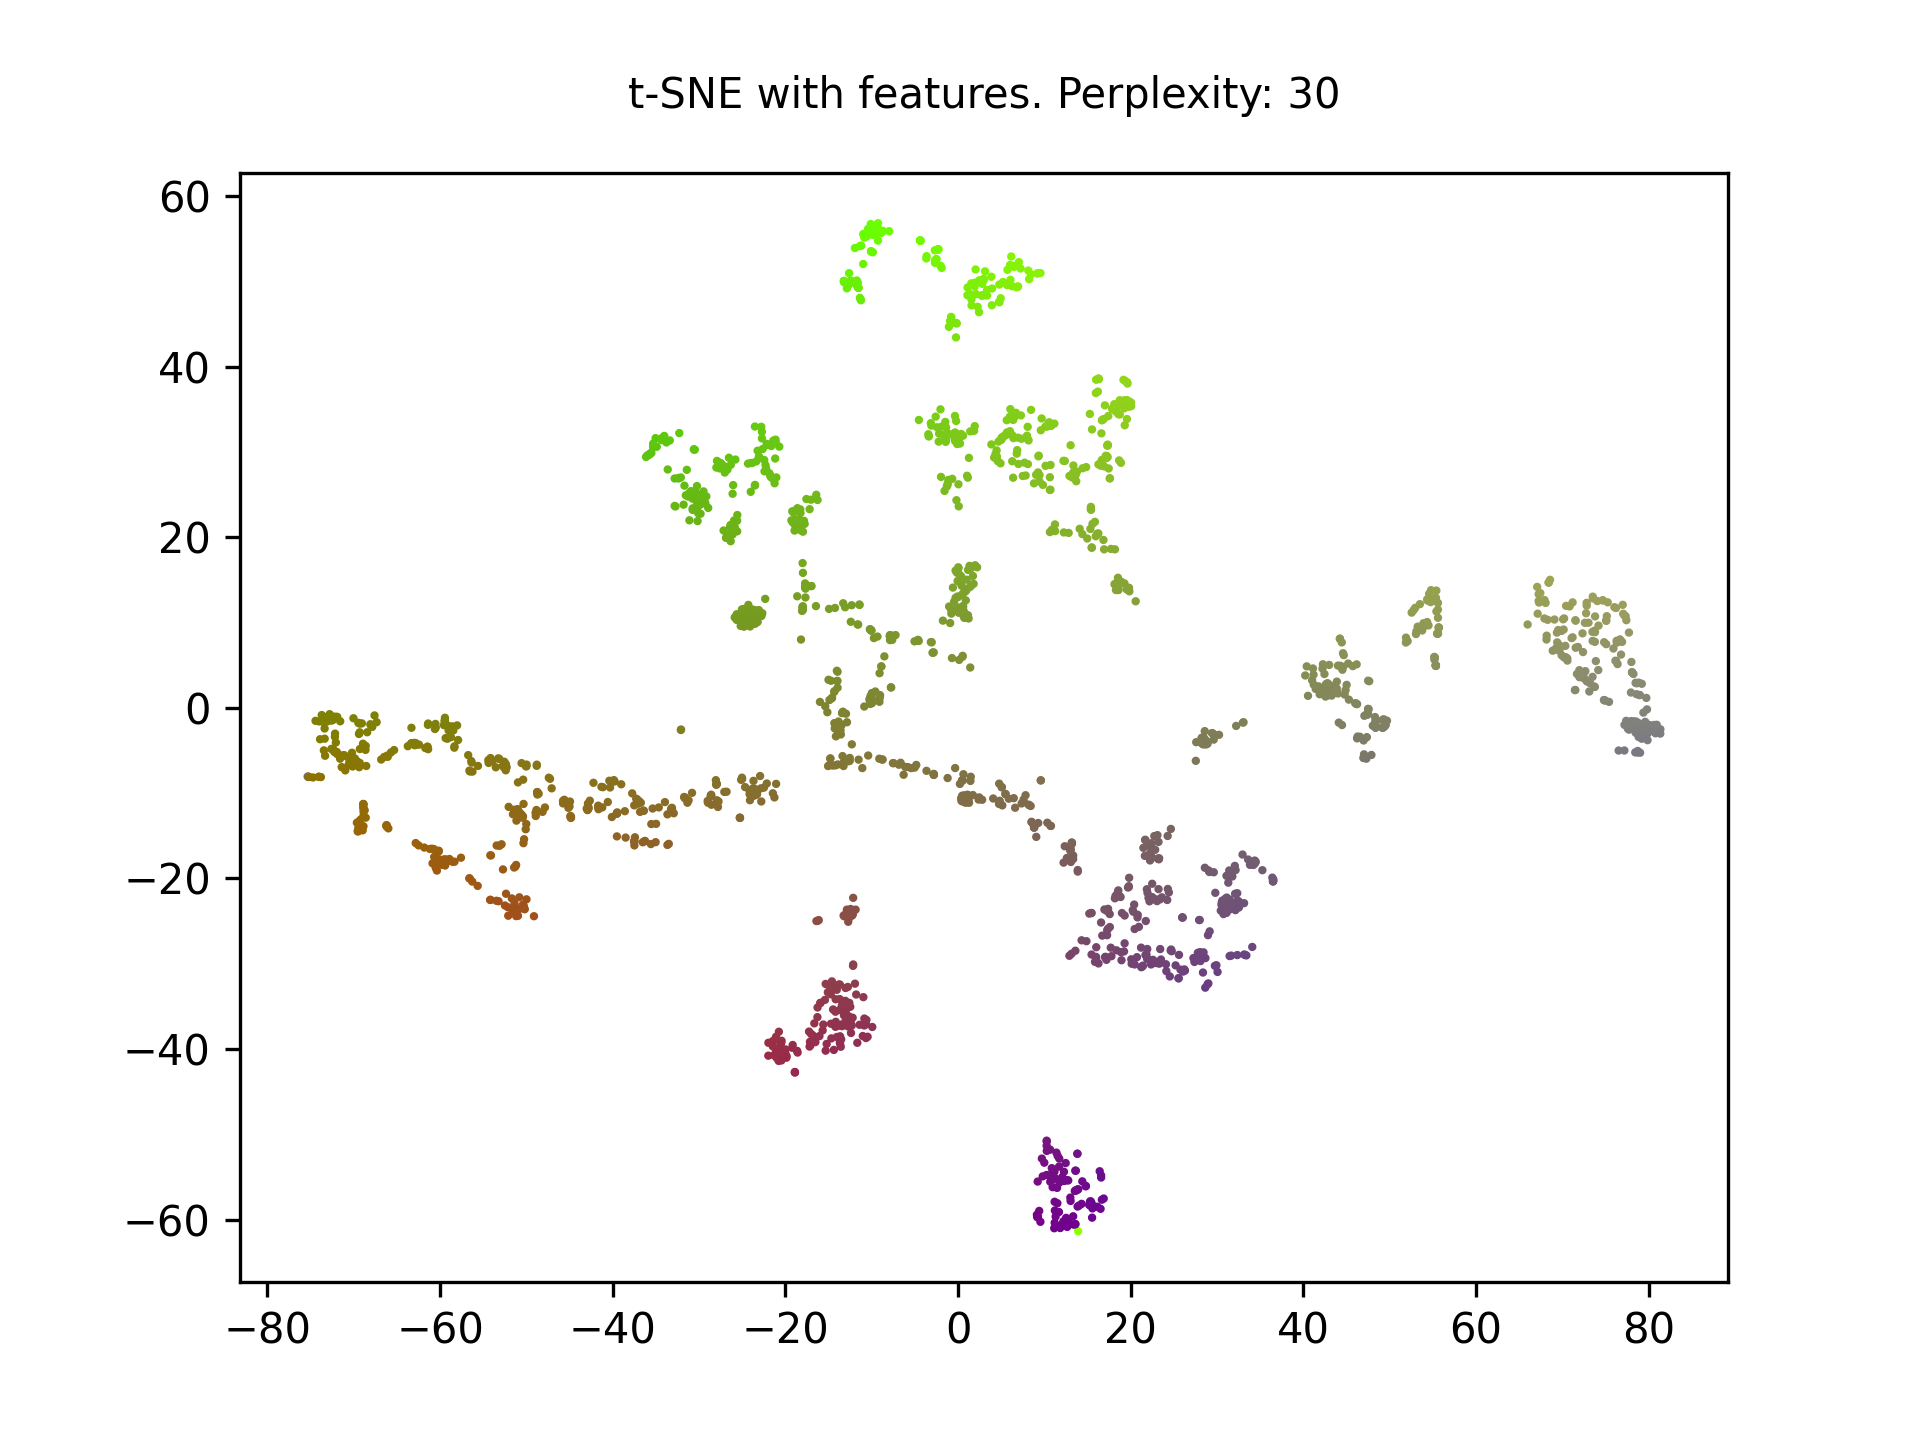
\includegraphics[width=0.45\textwidth]{images/tsne_gg_gl2vecAttr_features_p30.png}
    }
    \qquad
    \subfloat[Point-Line\label{fig:tsne_pointad_feature}]{
        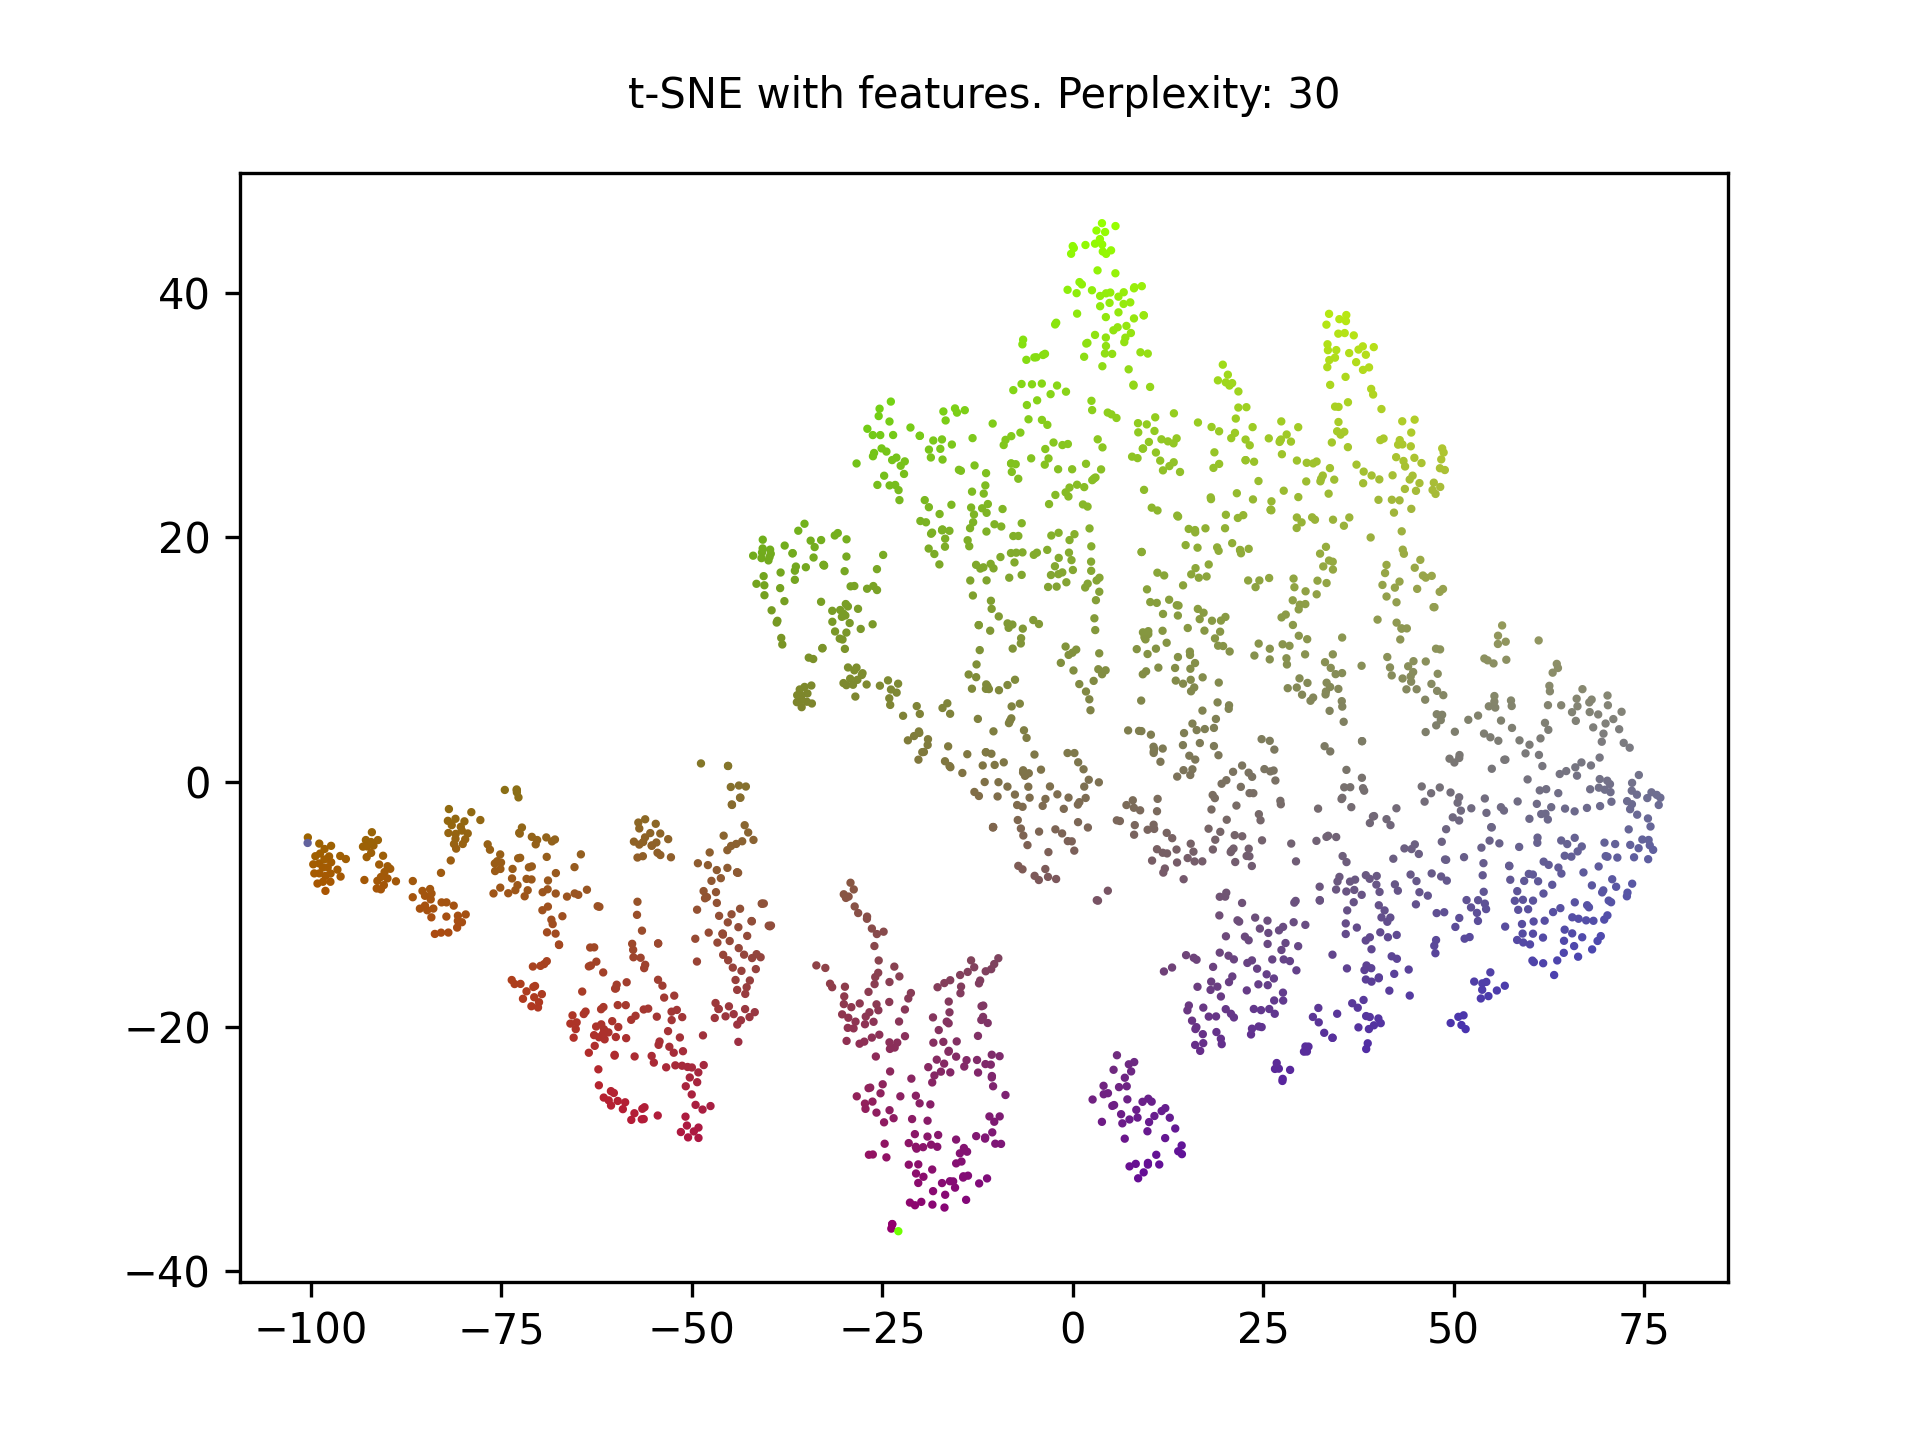
\includegraphics[width=0.45\textwidth]{images/tsne_pointad_gl2vecAttr_features_p30.png}
    }
    \qquad
    \subfloat[SMT Genome\label{fig:tsne_smt_feature}]{
        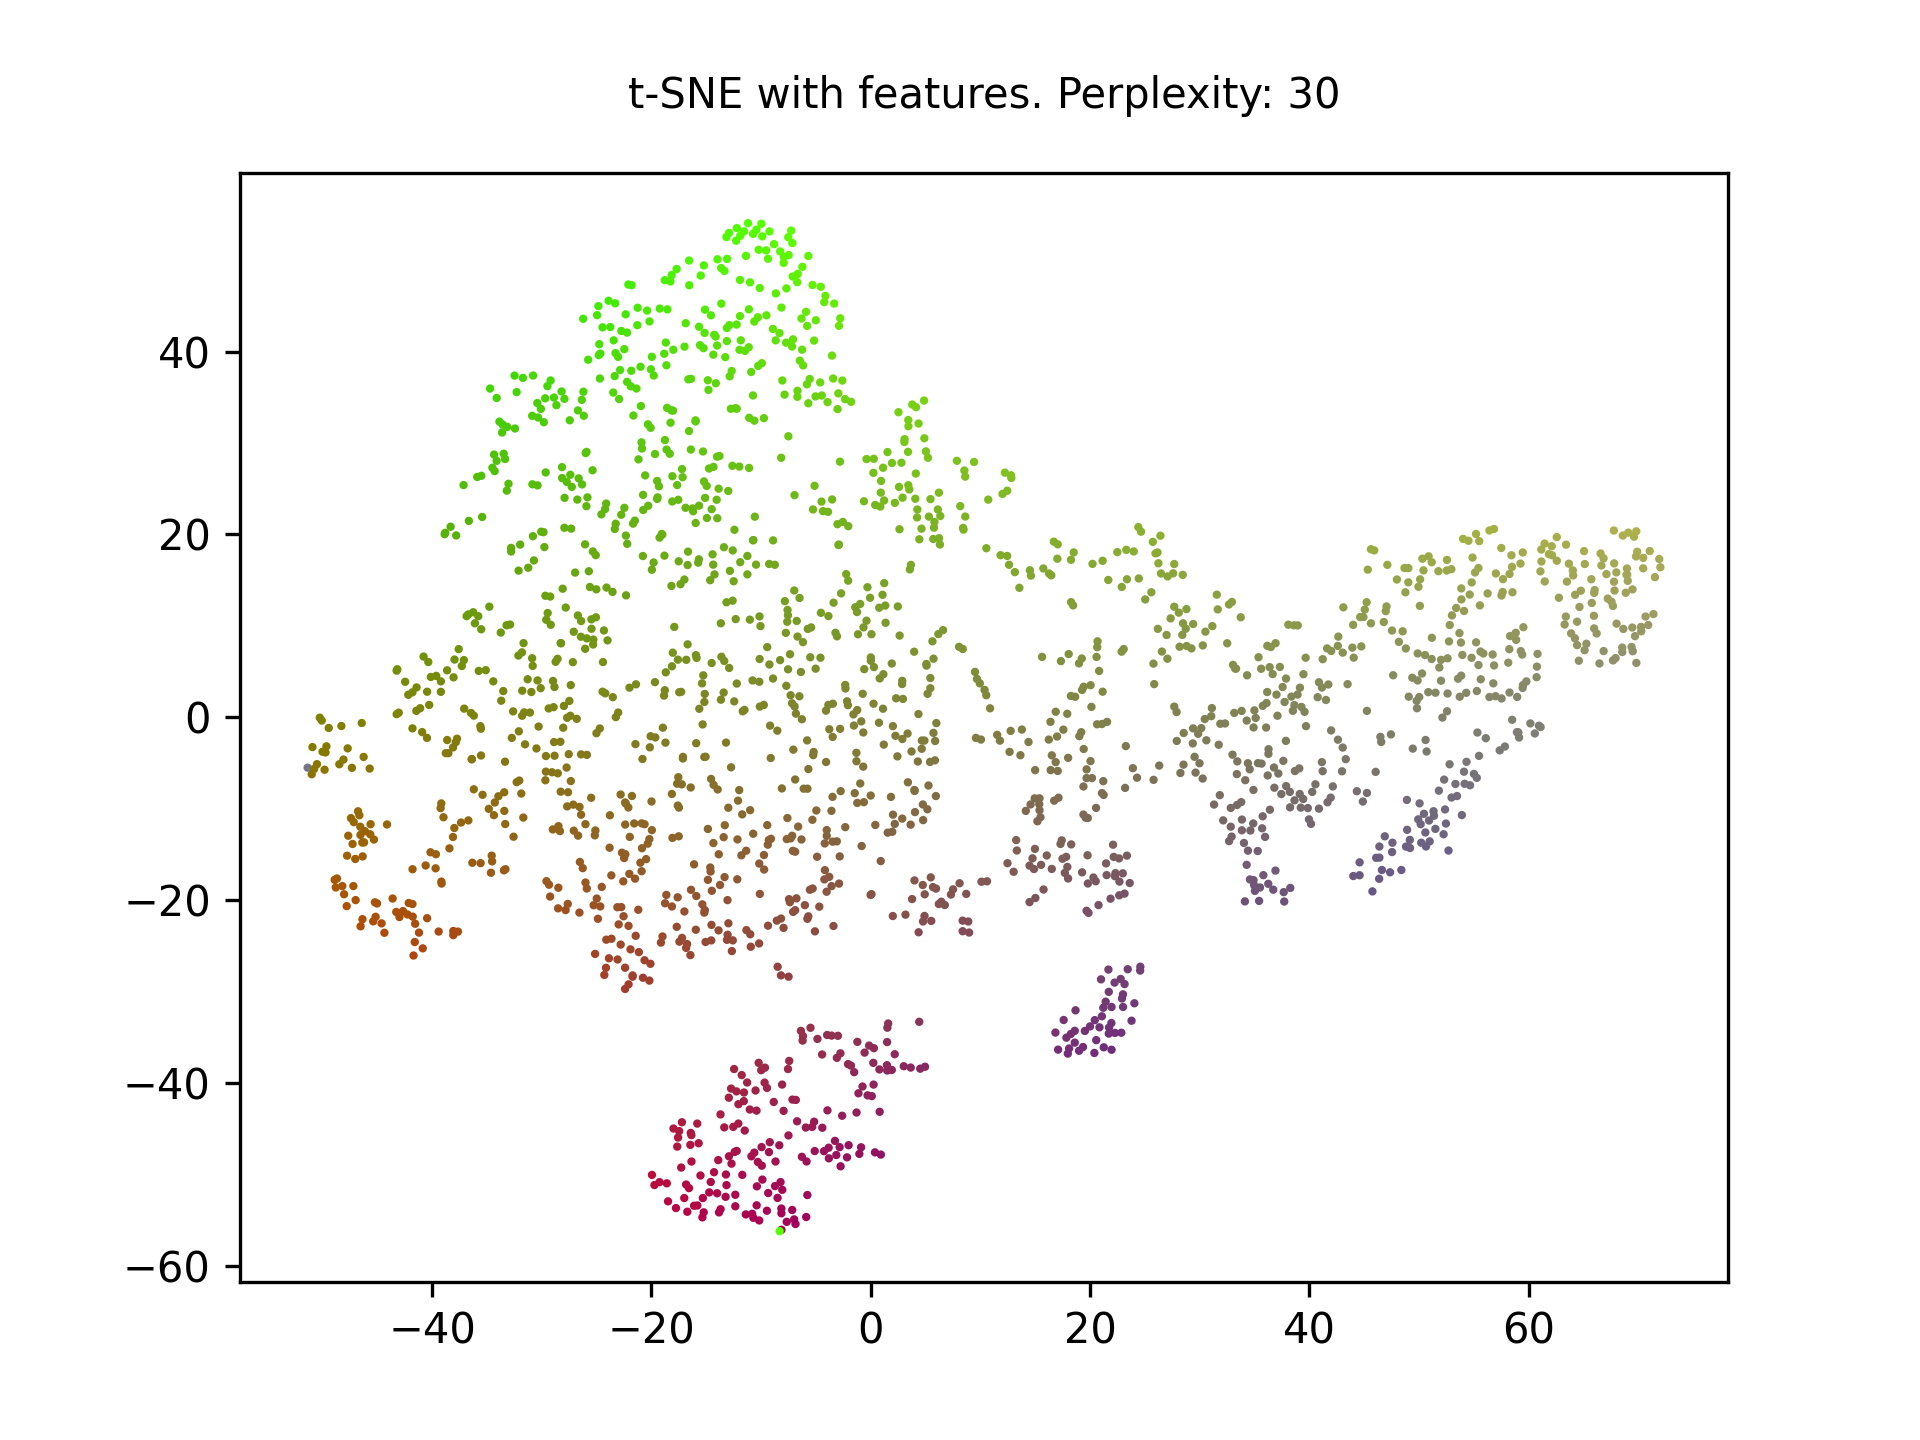
\includegraphics[width=0.45\textwidth]{images/tsne_smt_gl2vecAttr_features_p30.png}
    }
    \qquad
    \caption{t-SNE analysis of the features for each genome representation.}
    \label{fig:tsne_feature}
\end{figure}

From these results we can already observe that, while for \textit{All-Black}, \textit{Point-Line} and \textit{SMT Genome} the points are well distributed, for the \textit{Grid-Graph} representation points are clearly clustered; while other representation generate individuals whose varied features allow them to be placed continuously in the projected space, \textit{Grid-Graph} produces individuals whose features can be starkly categorized, leading to less variety. This result likely stems from the fact that the \textit{Grid-Graph} representation is the most simplistic, leading often to maps with similar designs and features.

\subsection{t-SNE of the image space}
We then applied \textit{t-SNE} using a different high-dimensional space from that of the features, namely the image space, described by the map's grid: each map is represented as an $NxM$ matrix where each cell contains 1 if the tile is walkable and 0 otherwise. We applied \textit{t-SNE} using the flattened matrices as vectors, projecting the $NxM$-dimensional space to 2 dimensions.

This analysis should cluster maps that are visually similar, and we will look for possible correlations between a map's appearance and its features. The results are shown in figure \cref{fig:tsne_images}, where each point is assigned the same color as in the plots in figure \cref{fig:tsne_feature}, meaning that similarly colored points represent maps with similar features.

\begin{figure}[hbt!]
    \centering
    \subfloat[All-black\label{fig:tsne_ab_img}]{
        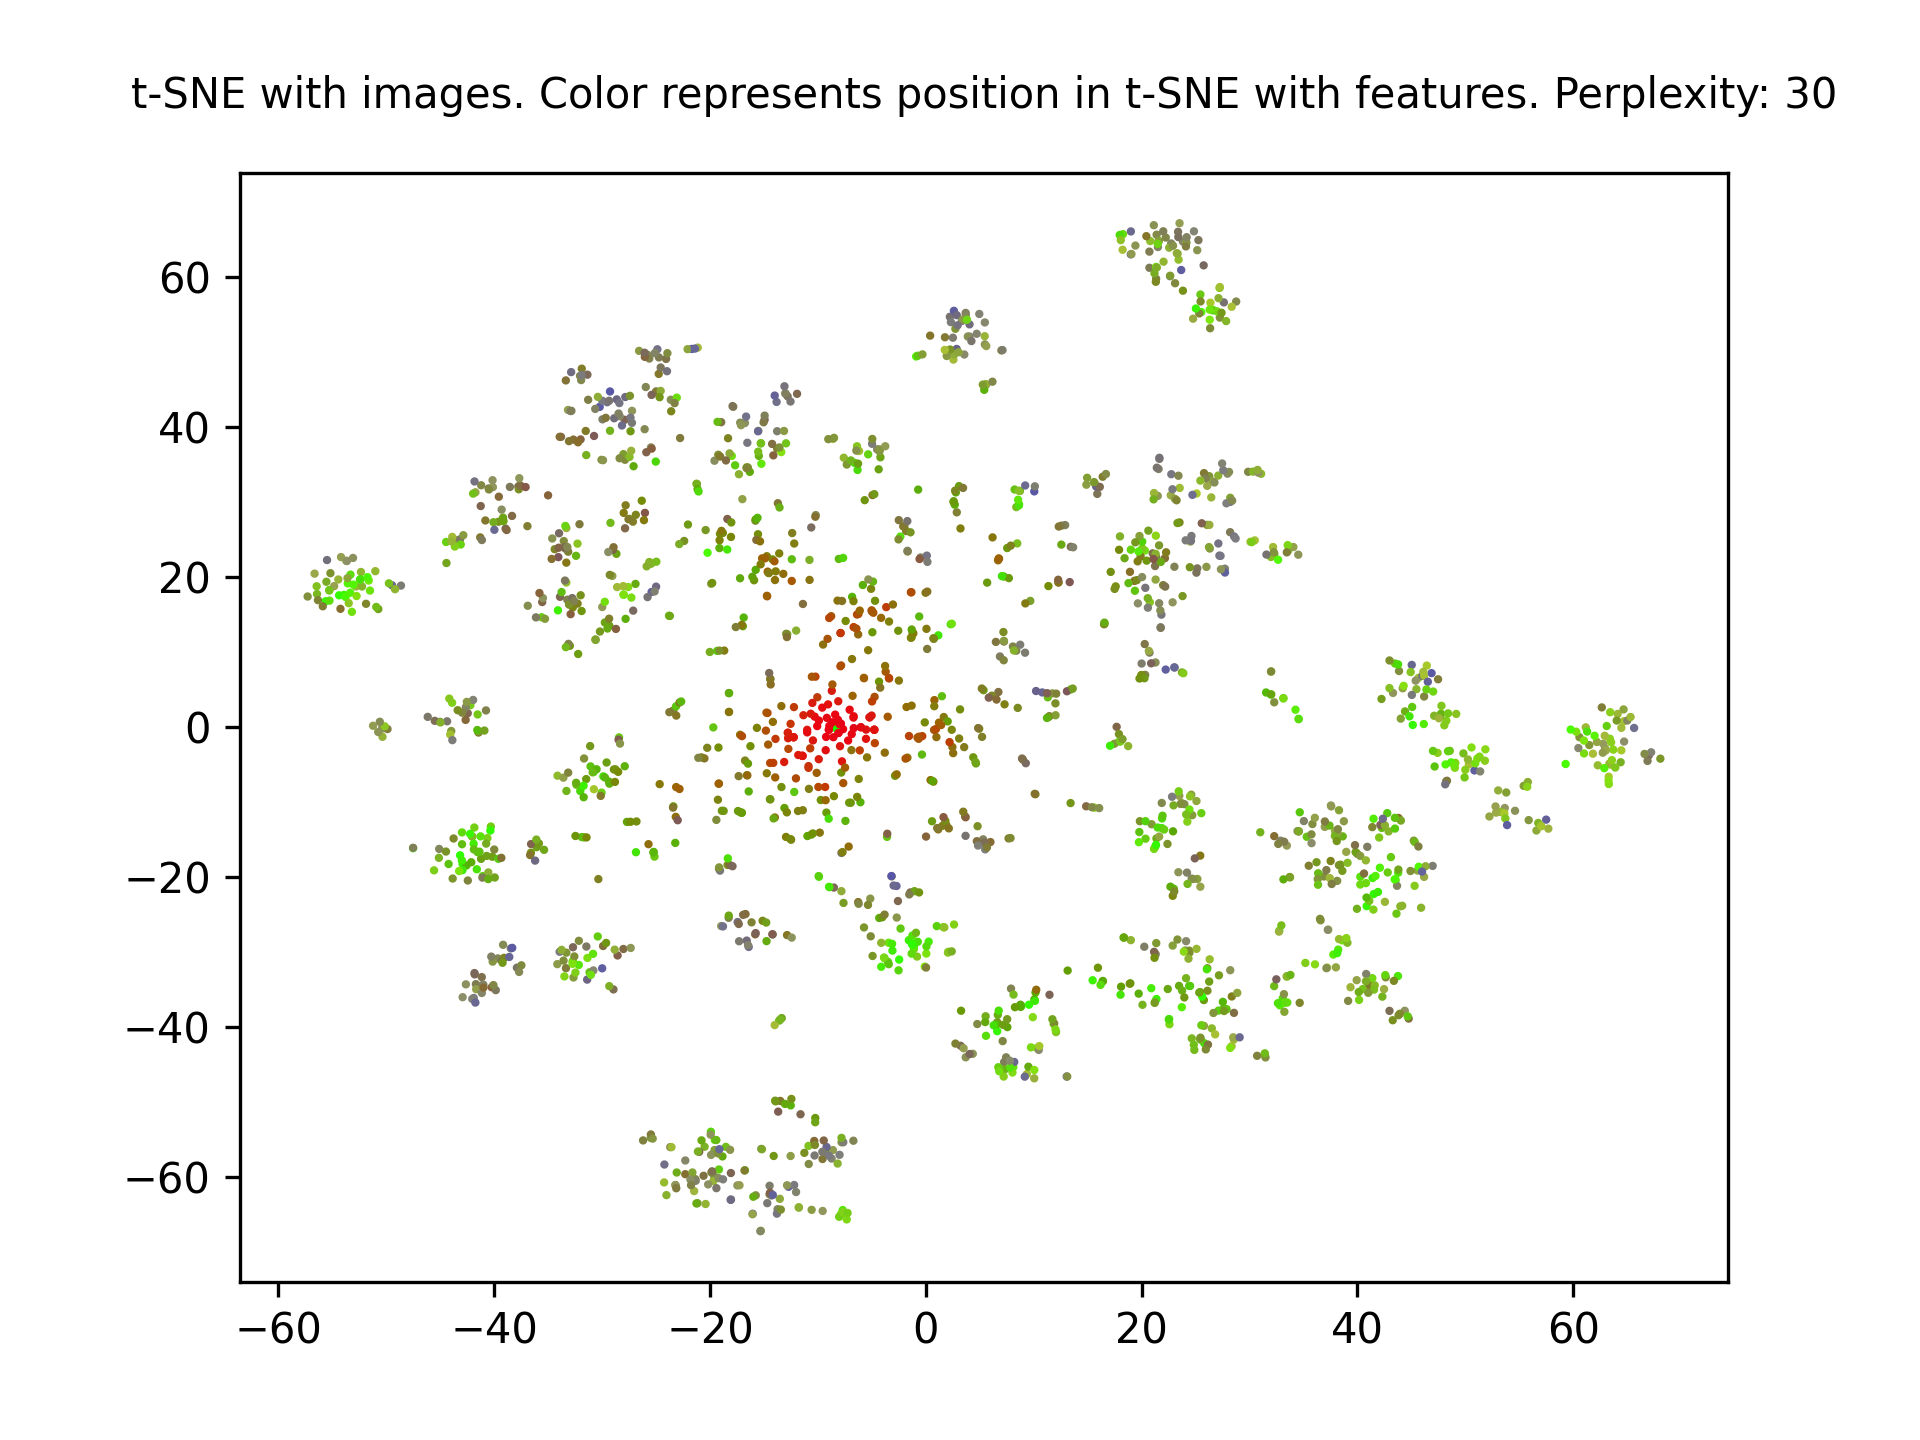
\includegraphics[width=0.45\textwidth]{images/tsne_ab_gl2vecAttr_img_p30.png}
    }
    \qquad
    \subfloat[Grid-Graph\label{fig:tsne_gg_img}]{
        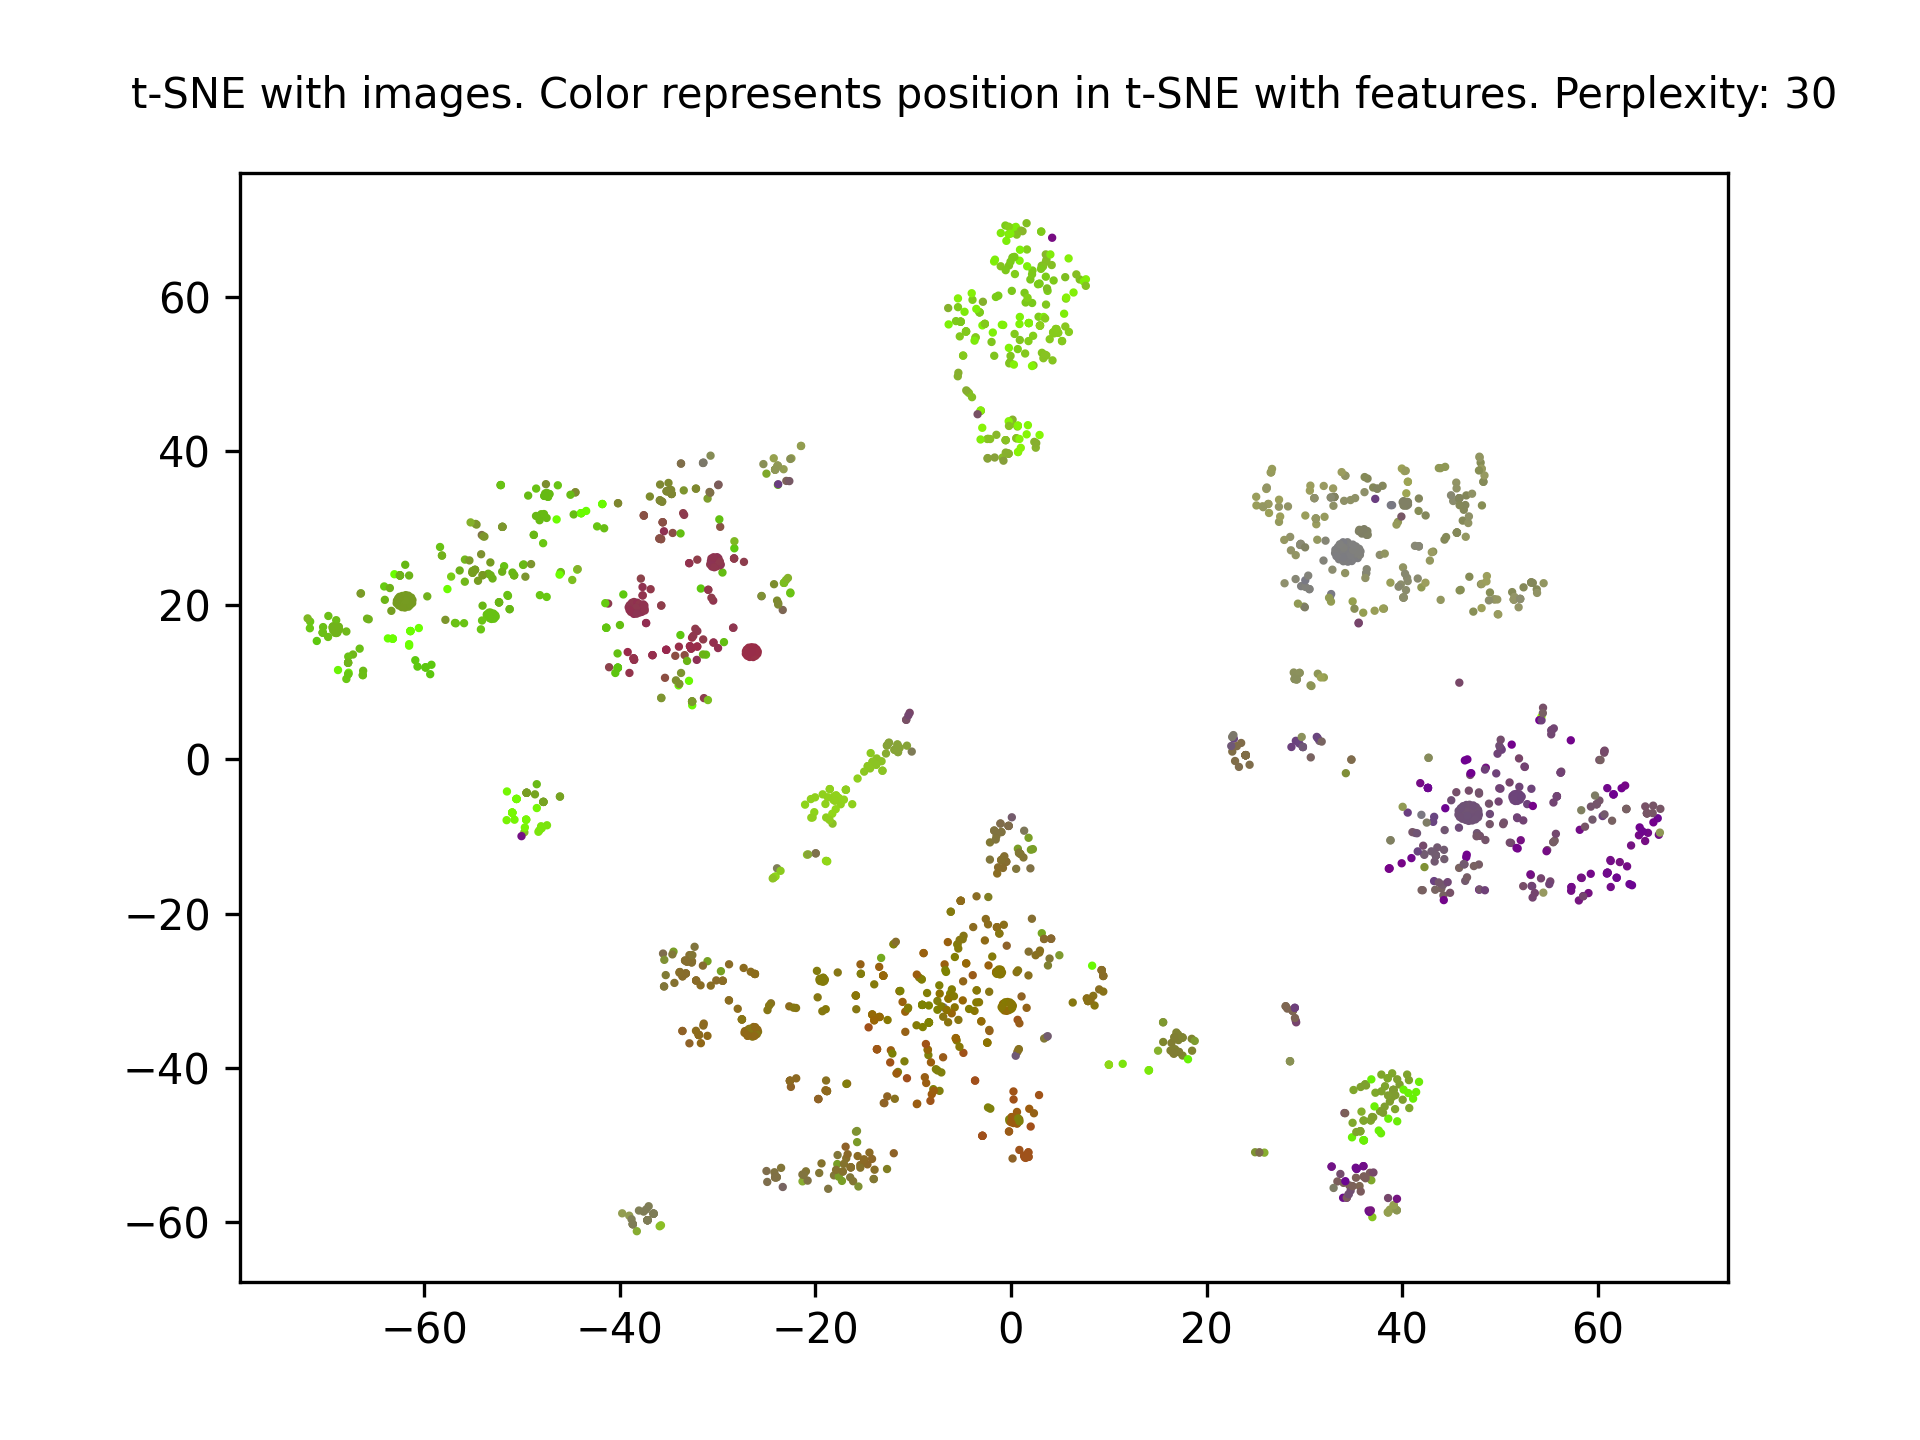
\includegraphics[width=0.45\textwidth]{images/tsne_gg_gl2vecAttr_img_p30.png}
    }
    \qquad
        \subfloat[Point-Line\label{fig:tsne_pointad_img}]{
        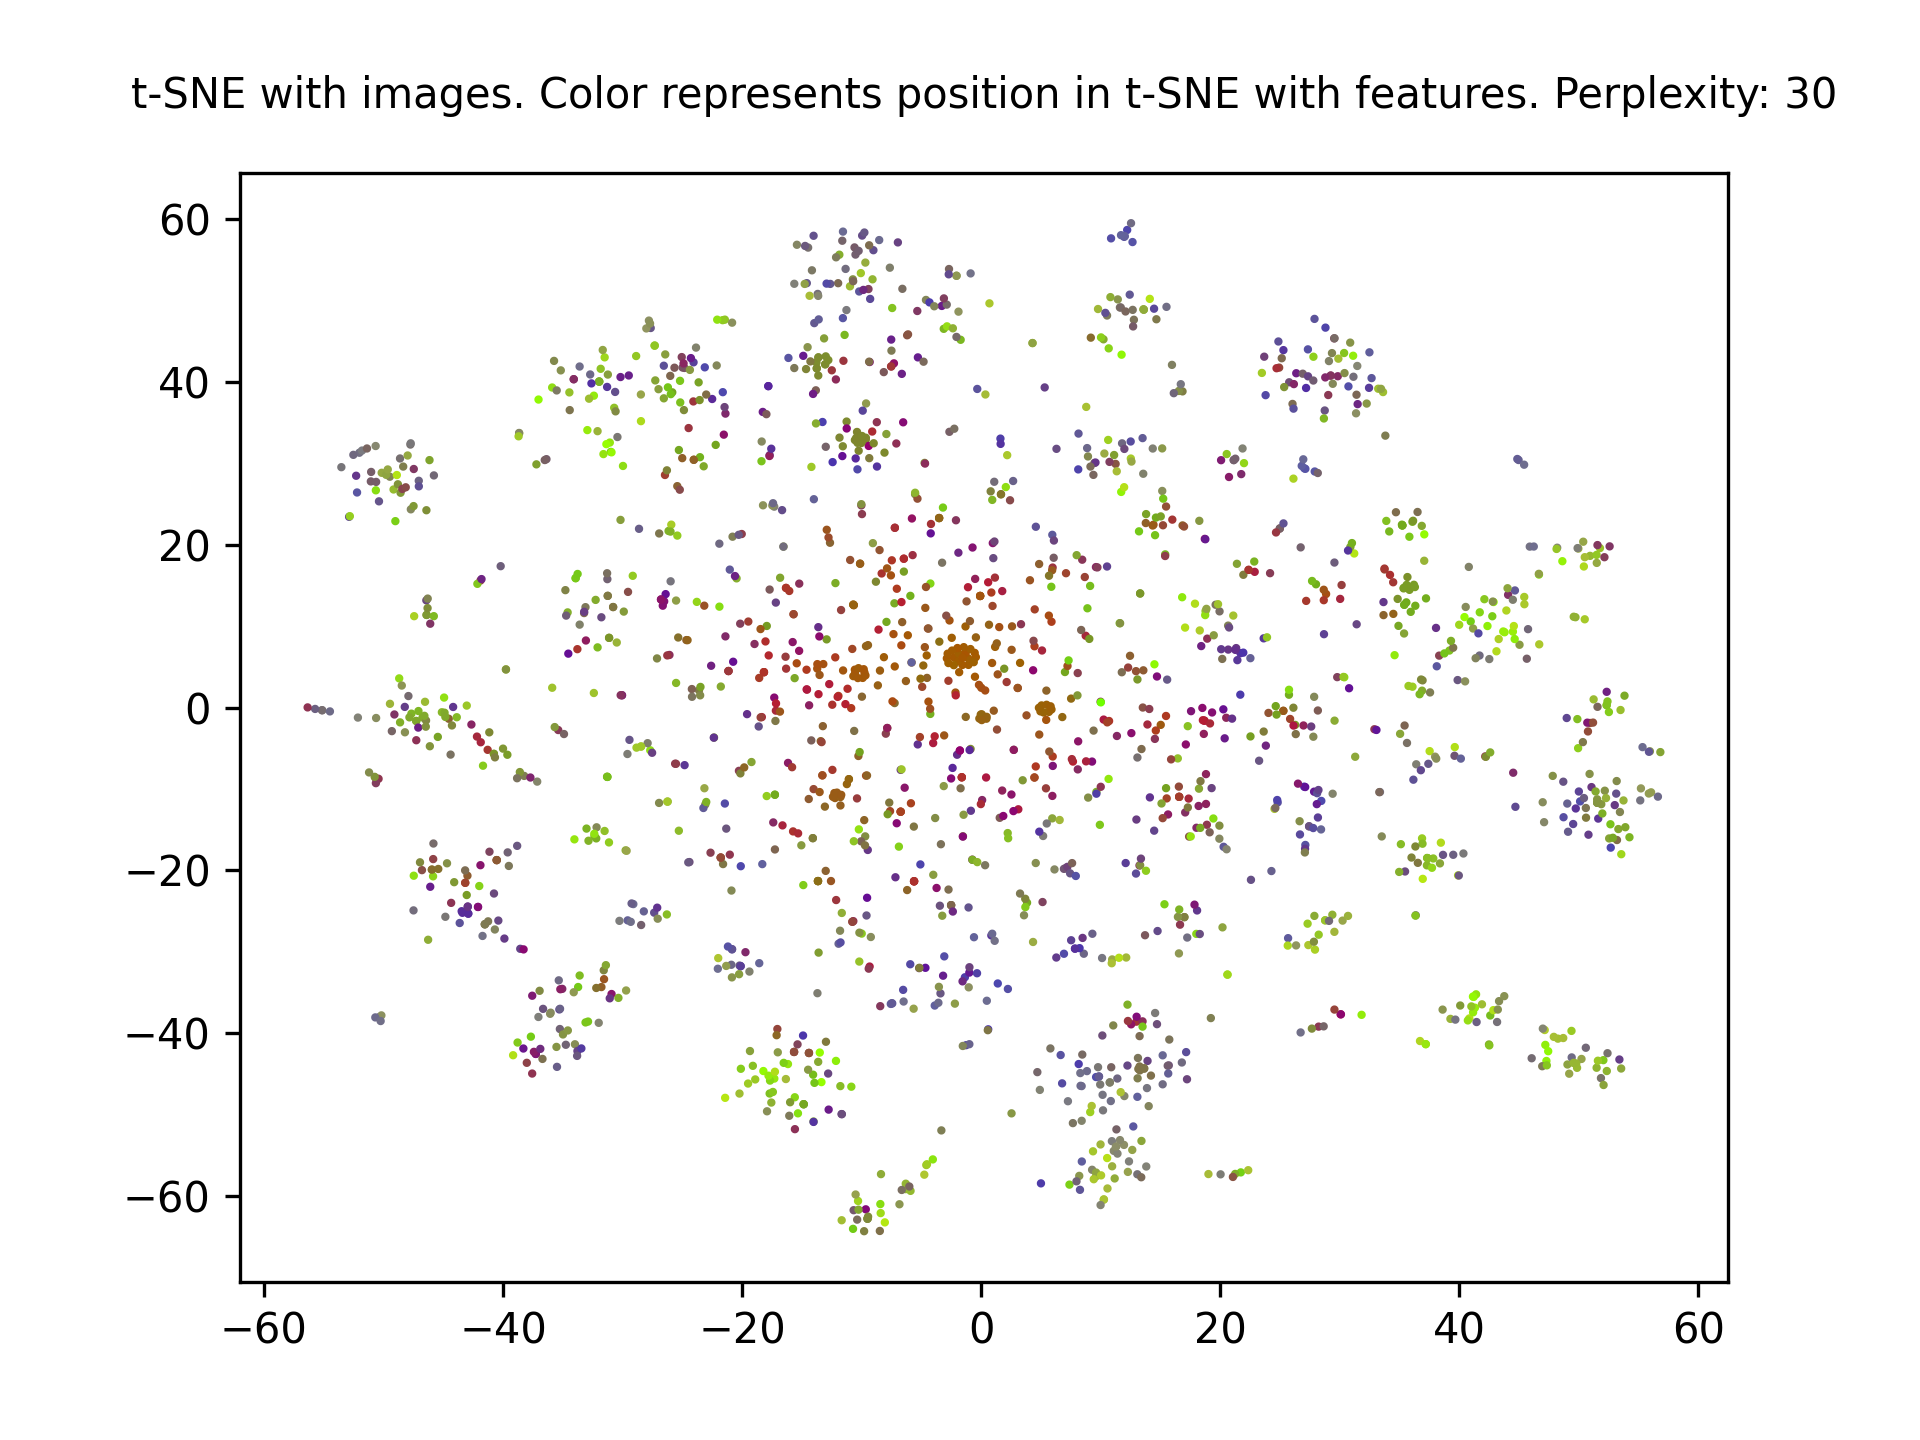
\includegraphics[width=0.45\textwidth]{images/tsne_pointad_gl2vecAttr_img_p30.png}
    }
    \qquad
    \subfloat[SMT Genome\label{fig:tsne_smt_img}]{
        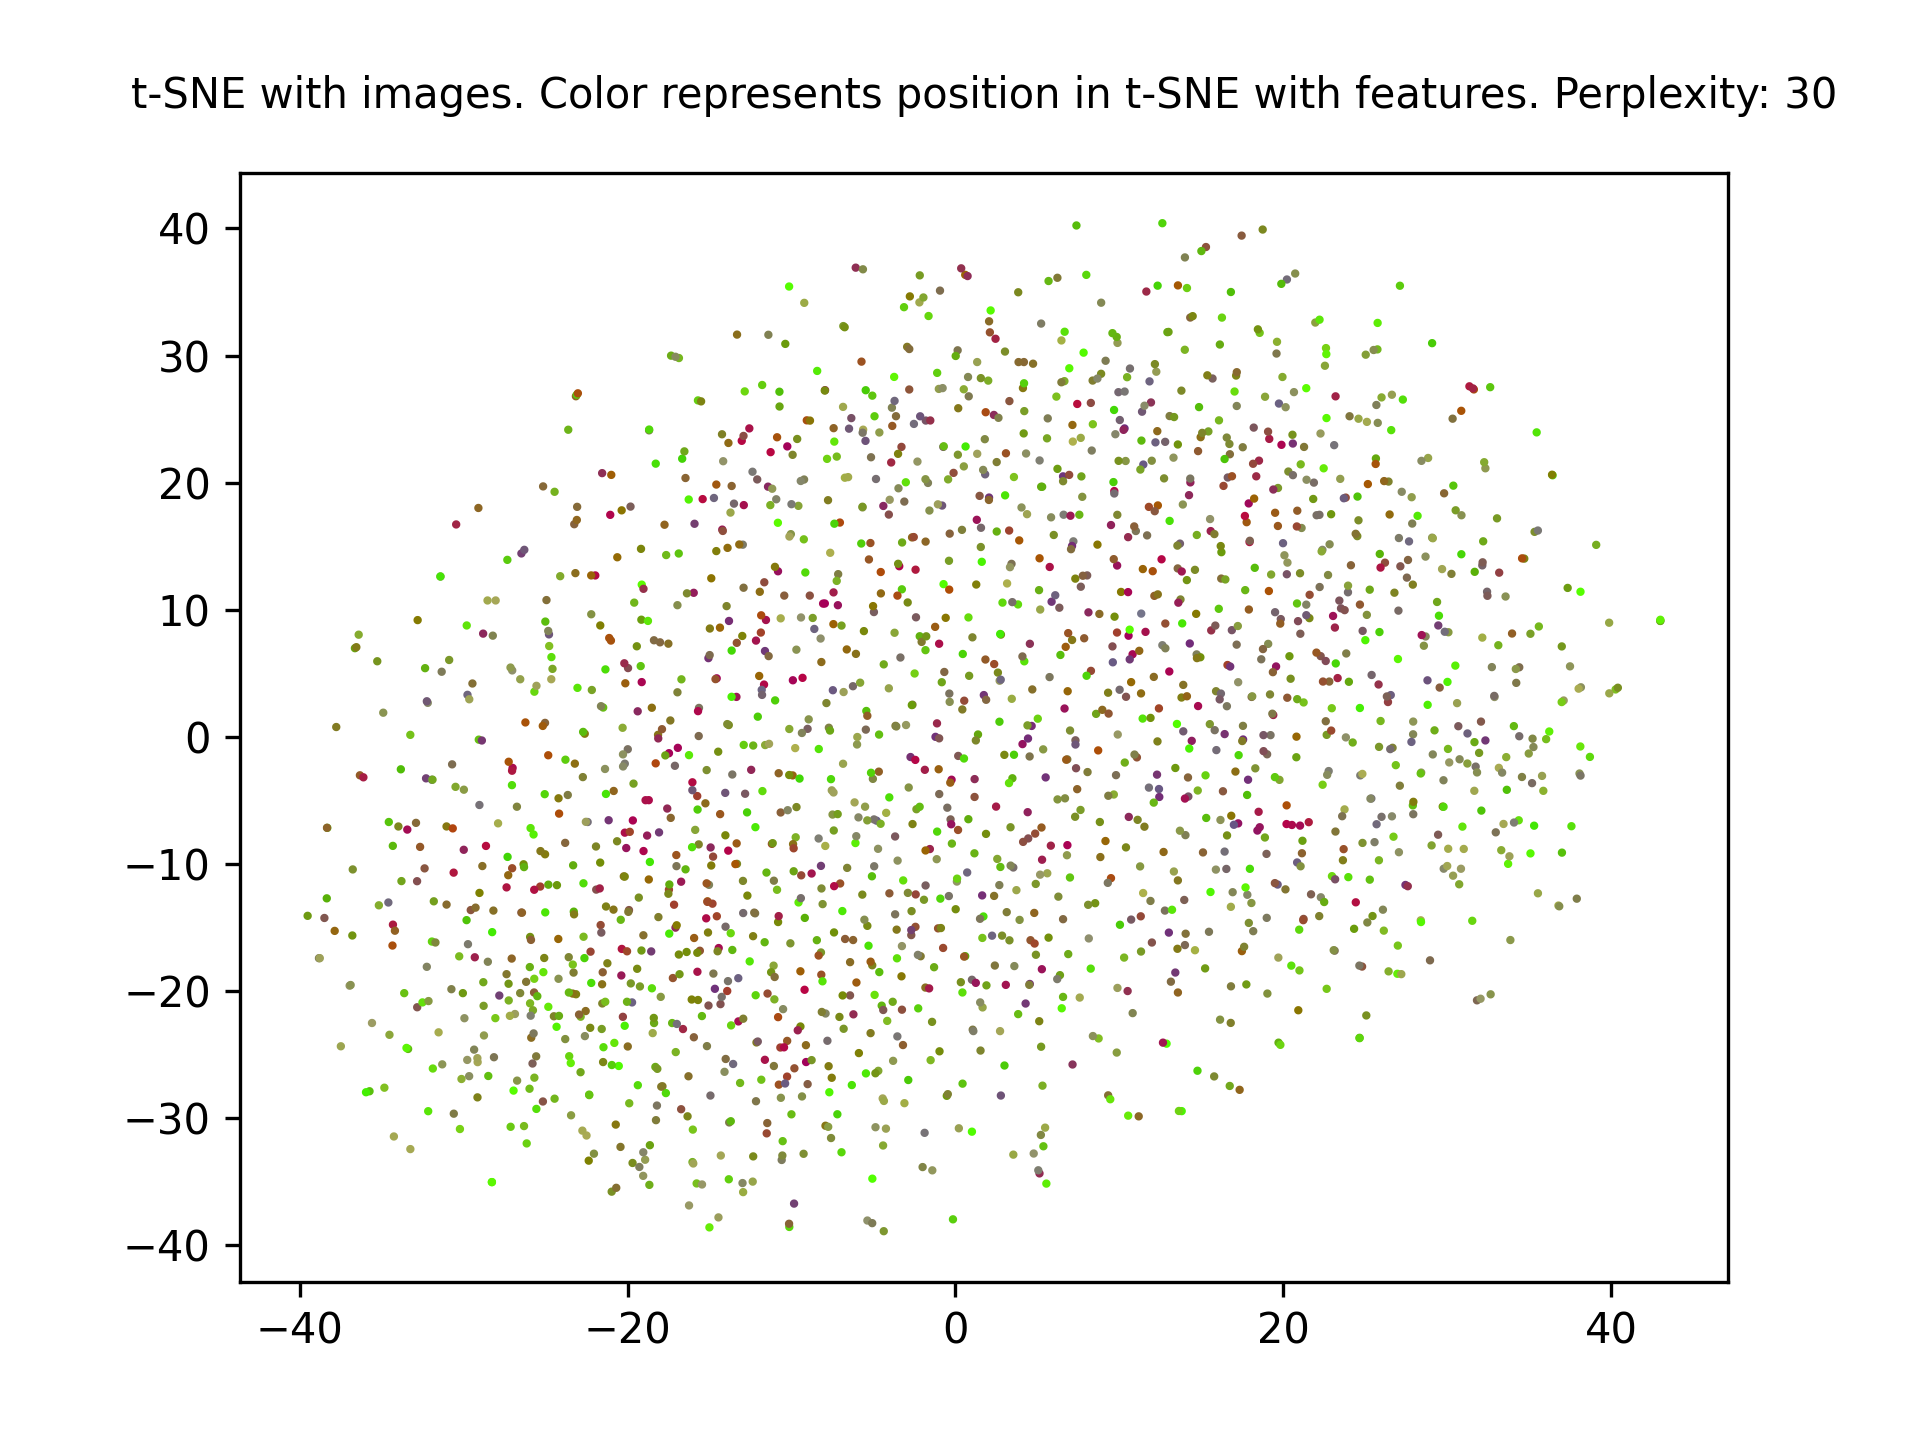
\includegraphics[width=0.45\textwidth]{images/tsne_smt_gl2vecAttr_img_p30.png}
    }
    \qquad
    \caption{t-SNE analysis of the images for each genome representation.}
    \label{fig:tsne_images}
\end{figure}

Before analyzing the results, we wanted to ensure that maps close in the space projected by \textit{t-SNE} are actually visually similar. To do so, we empirically examined the maps corresponding to the points in the plot, and we include some examples in figure \cref{fig:tsne_images_examples}. We confirmed that maps that are close are indeed similar, in that they share a similar shape, while not sharing necessarily the topological structure of the map. This makes sense as two very similar maps may differ by a single tile which when removed changes the connections between rooms, but not the overall visual shape of the map.

\begin{figure}[hbt!]
    \centering
    \subfloat[0, 0]{
        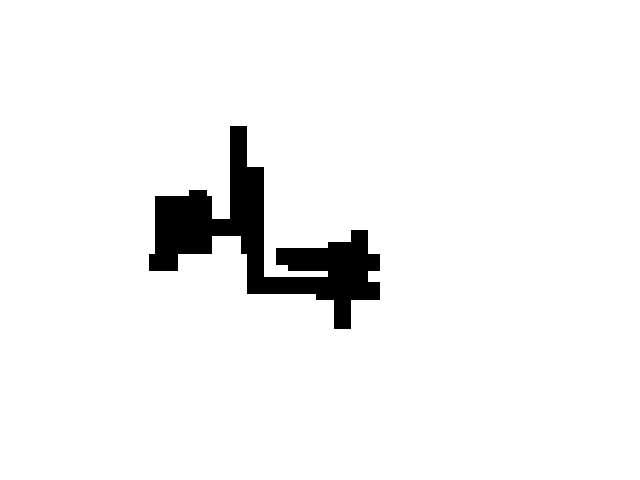
\includegraphics[width=0.22\textwidth]{images/tsne_samples/img11.png}
        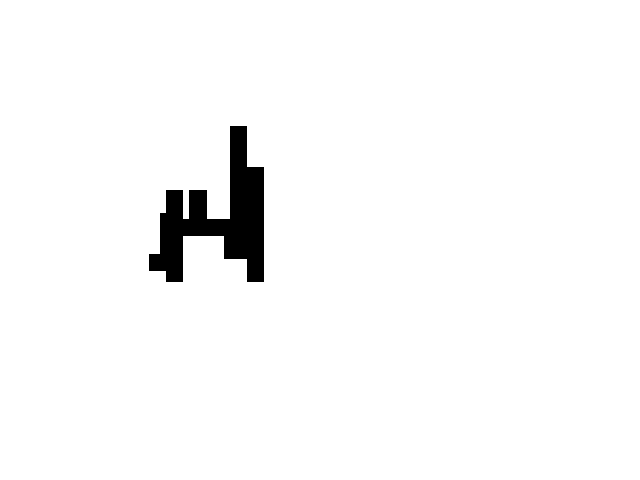
\includegraphics[width=0.22\textwidth]{images/tsne_samples/img12.png}
    }
    \qquad
    \subfloat[60, 0]{
        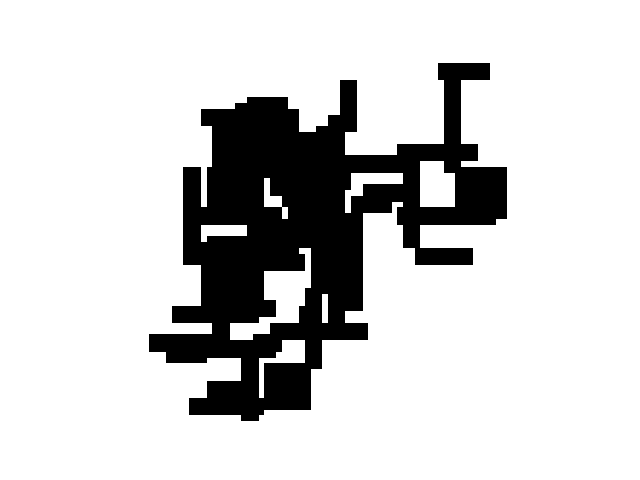
\includegraphics[width=0.22\textwidth]{images/tsne_samples/img21.png}
        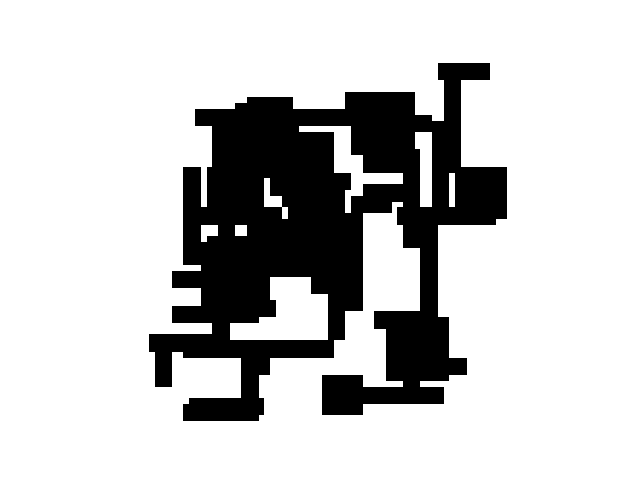
\includegraphics[width=0.22\textwidth]{images/tsne_samples/img22.png}
    }
    \qquad
    \subfloat[18, 65]{
        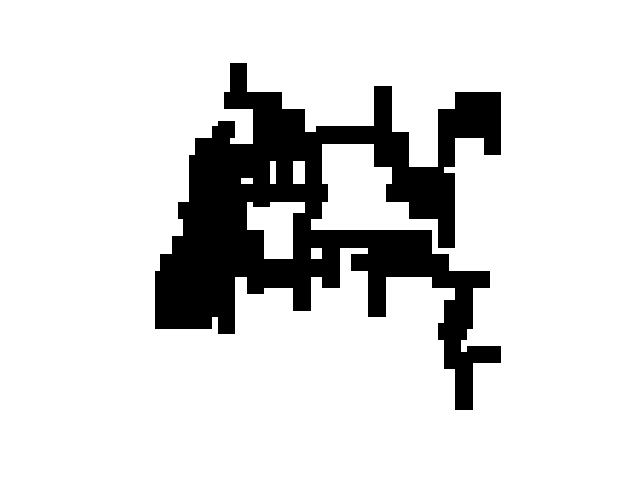
\includegraphics[width=0.22\textwidth]{images/tsne_samples/img31.png}
        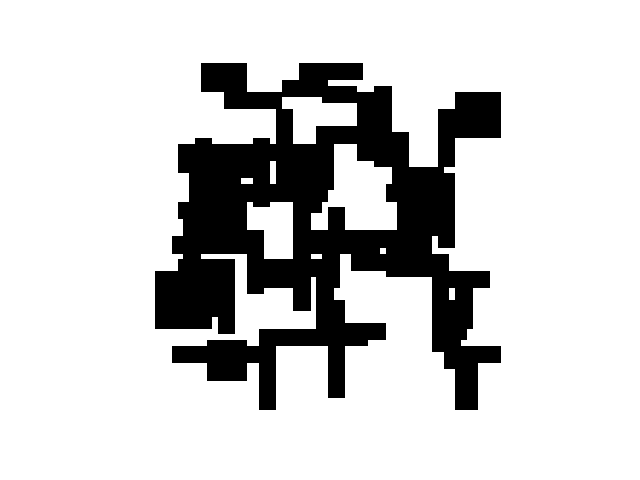
\includegraphics[width=0.22\textwidth]{images/tsne_samples/img32.png}
    }
    \qquad
    \subfloat[-56, 18]{
        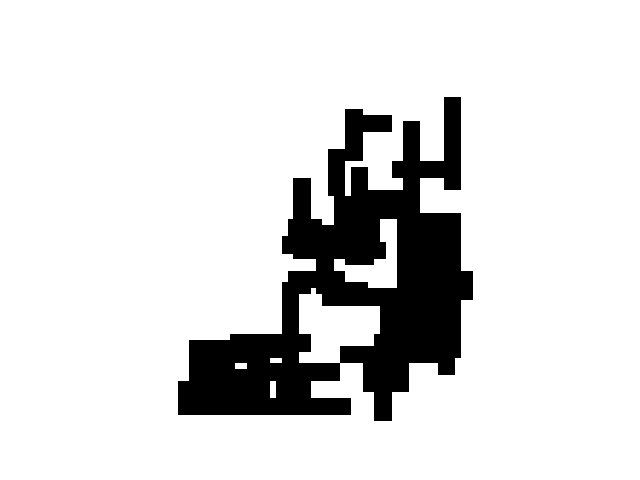
\includegraphics[width=0.22\textwidth]{images/tsne_samples/img41.png}
        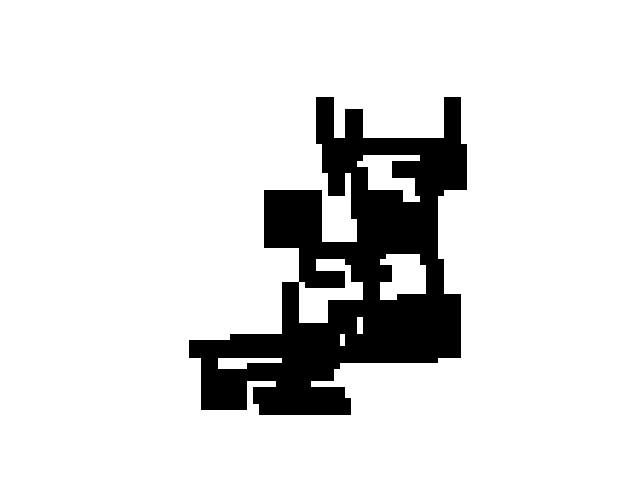
\includegraphics[width=0.22\textwidth]{images/tsne_samples/img42.png}
    }
    \qquad
    \subfloat[0, -32]{
        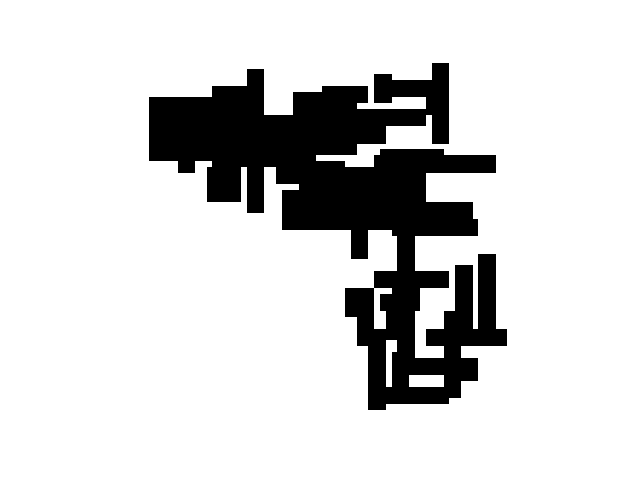
\includegraphics[width=0.22\textwidth]{images/tsne_samples/img51.png}
        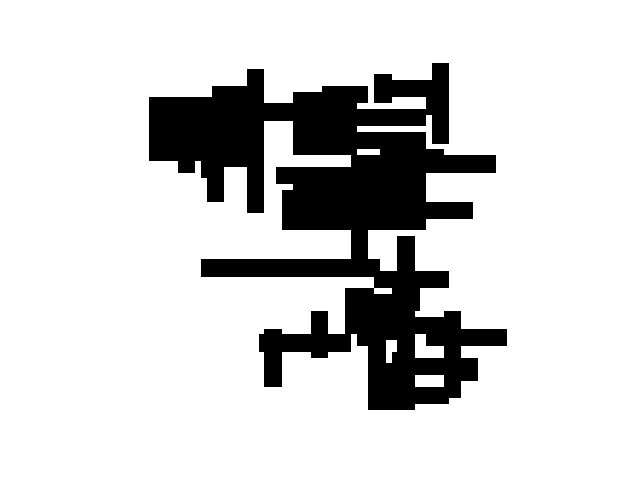
\includegraphics[width=0.22\textwidth]{images/tsne_samples/img52.png}
    }
    \qquad
    \subfloat[-26, -55]{
        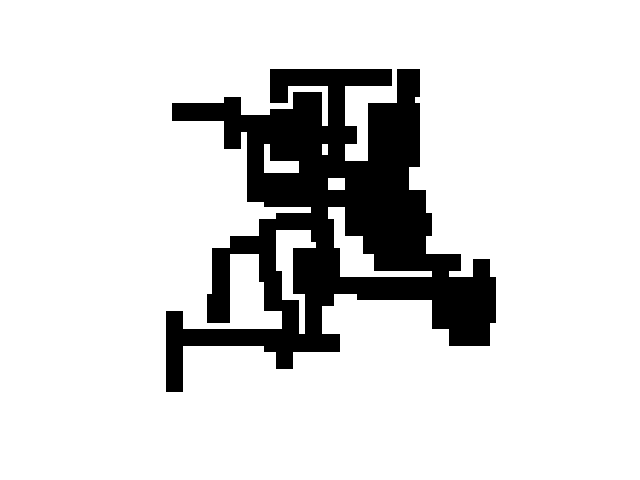
\includegraphics[width=0.22\textwidth]{images/tsne_samples/img61.png}
        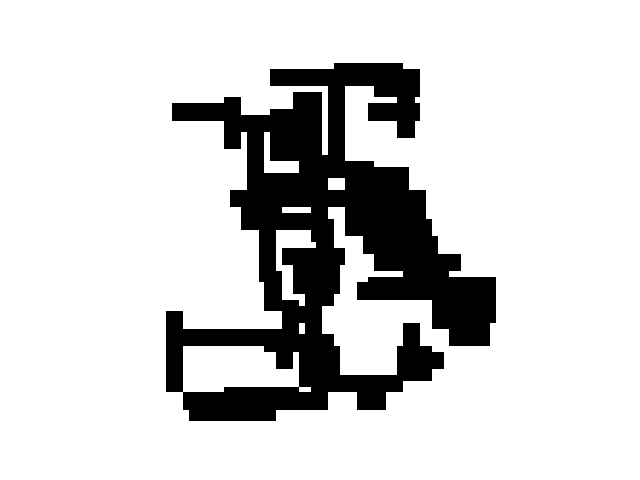
\includegraphics[width=0.22\textwidth]{images/tsne_samples/img62.png}
    }
    \caption[t-SNE image similarity examples]{Samples of random couples of points close in the space projected by \textit{t-SNE} for the All-Black representation, chosen to make an example. We report to the approximate location of each couple. We can clearly see that the maps are visually similar.}
    \label{fig:tsne_images_examples}
\end{figure}

We notice that the \textit{Grid-Graph} representation (fig. \cref{fig:tsne_gg_img}) presents the strongest clustering, with also colors being more clustered, leading us to believe that there exists a correlation between features and visual appearance. This is not the case for the other representations, where the clustering is less pronounced, and colors are more scattered. The \textit{SMT Genome} representation (fig. \cref{fig:tsne_smt_img}) is the most scattered, which suggests that the \textit{SMT Genome} representation allows for the generation of a wide variety of maps, whose visual appearance gives little to no insight on their features.

To further investigate the correlation between features and visual appearance we have analyzed the distance between each couple of points in both the spaces projected by \textit{t-SNE}. The result of this analysis can be seen in the graph in figure \cref{fig:tsne_distance}, obtained by plotting a point for each couple of maps; the x-axis represents the distance in the projected feature space of these two maps while the y-axis represents the distance in the projected image space.

\begin{figure}[hbt!]
    \centering
    \subfloat[All-black\label{fig:tsne_ab_distance}]{
        \includegraphics[width=0.45\textwidth]{images/tsne_ab_gl2vecAttr_disttsne_feat_img_p30.png}
    }
    \qquad
    \subfloat[Grid-Graph\label{fig:tsne_gg_distance}]{
        \includegraphics[width=0.45\textwidth]{images/tsne_gg_gl2vecAttr_disttsne_feat_img_p30.png}
    }
    \qquad
    \subfloat[Point-Line\label{fig:tsne_pointad_distance}]{
        \includegraphics[width=0.45\textwidth]{images/tsne_pointad_gl2vecAttr_disttsne_feat_img_p30.png}
    }
    \qquad
    \subfloat[SMT Genome\label{fig:tsne_smt_distance}]{
        \includegraphics[width=0.45\textwidth]{images/tsne_smt_gl2vecAttr_disttsne_feat_img_p30.png}
    }
    \qquad
    \caption{Scatter plot of the distances in the feature space and in the image space.}
    \label{fig:tsne_distance}
\end{figure}

Only for the \textit{Grid-Graph} genome we can spot a soft correlation between the distances in the two spaces, which is expected from our previous observations. Other representations sport no such correlation.

This results overall suggest that visual appearance of a map is not a good indicator of its features, given that visually very similar maps may have very different features. While this result, or lack thereof, is in itself interesting, it does not help us in our goal of identifying significant features to be used in a QD approach.

\subsection{t-SNE of the latent space of the gl2Vec graph embedding}
\label{subsec:tsne_graphs}

As we noted, similar looking maps may have vastly different topologies; this observation led us to believe that looking for similar \textit{graphs} instead of similar \textit{images} may be more fruitful. To apply \textit{t-SNE} to the space of graphs, we need to use an encoding such that any graph can be represented as a point in a high-dimensional space. We have used the \textit{gl2Vec}, a whole-graph embedding algorithm\footnote{Methods which aim at representing a whole graphs as vectors, such that structurally similar graphs are close in the embedding space.}, to encode each map's graph as a vector of values. We utilized \textit{karateclub}'s implementation\footnote{\url{https://karateclub.readthedocs.io/en/latest/modules/root.html\#karateclub.graph_embedding.gl2vec.GL2Vec}}, specially modified so that edges' lengths can be used as attributes. 

The fine-tuning of some \textit{gl2Vec} parameters may change the quality of the output. We empirically found that we obtained the best results using 640 \textit{dimensions} for the vectors, 2 \textit{Weisfeiler-Lehman iterations}, 10 \textit{epochs}, 0.0001 \textit{down-sampling frequency} and 0.025 \textit{learning rate}.

\textit{t-SNE} has been applied to the vectors obtained from the \textit{gl2Vec} embedding, reducing the 640-dimensional space to 2 dimensions (fig. \cref{fig:tsne_graphs}). Each point represents a map, and the color represents the position in the \textit{t-SNE} of the features (see fig. \cref{fig:tsne_feature}).

\begin{figure}[hbt!]
    \centering
    \subfloat[All-black\label{fig:tsne_ab_graph}]{
        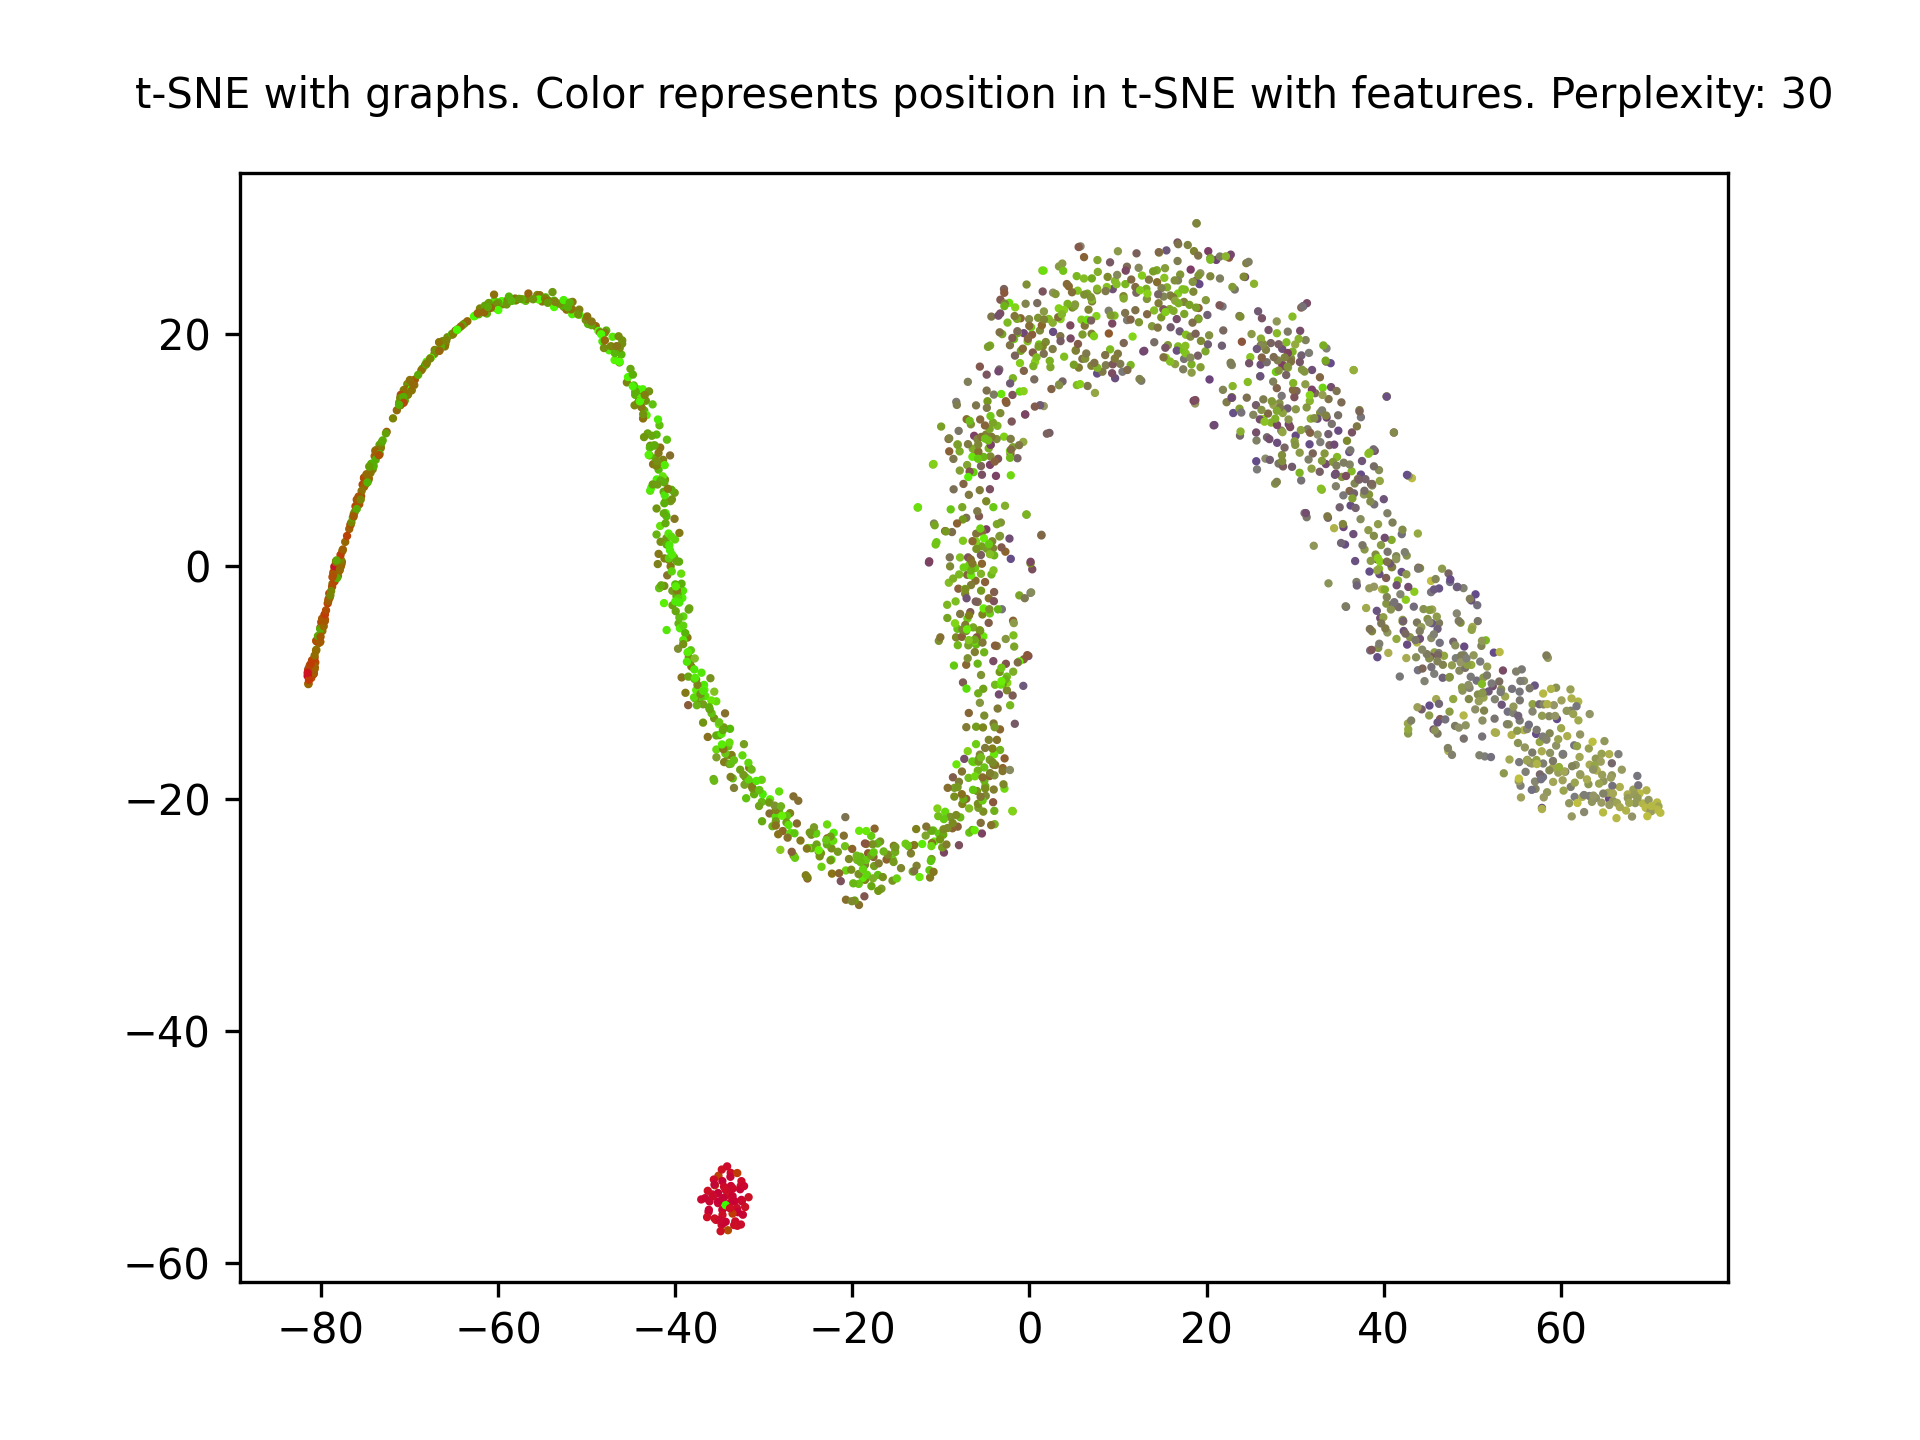
\includegraphics[width=0.45\textwidth]{images/tsne_ab_gl2vecAttr_graph_p30.png}
    }
    \qquad
    \subfloat[Grid-Graph\label{fig:tsne_gg_graph}]{
        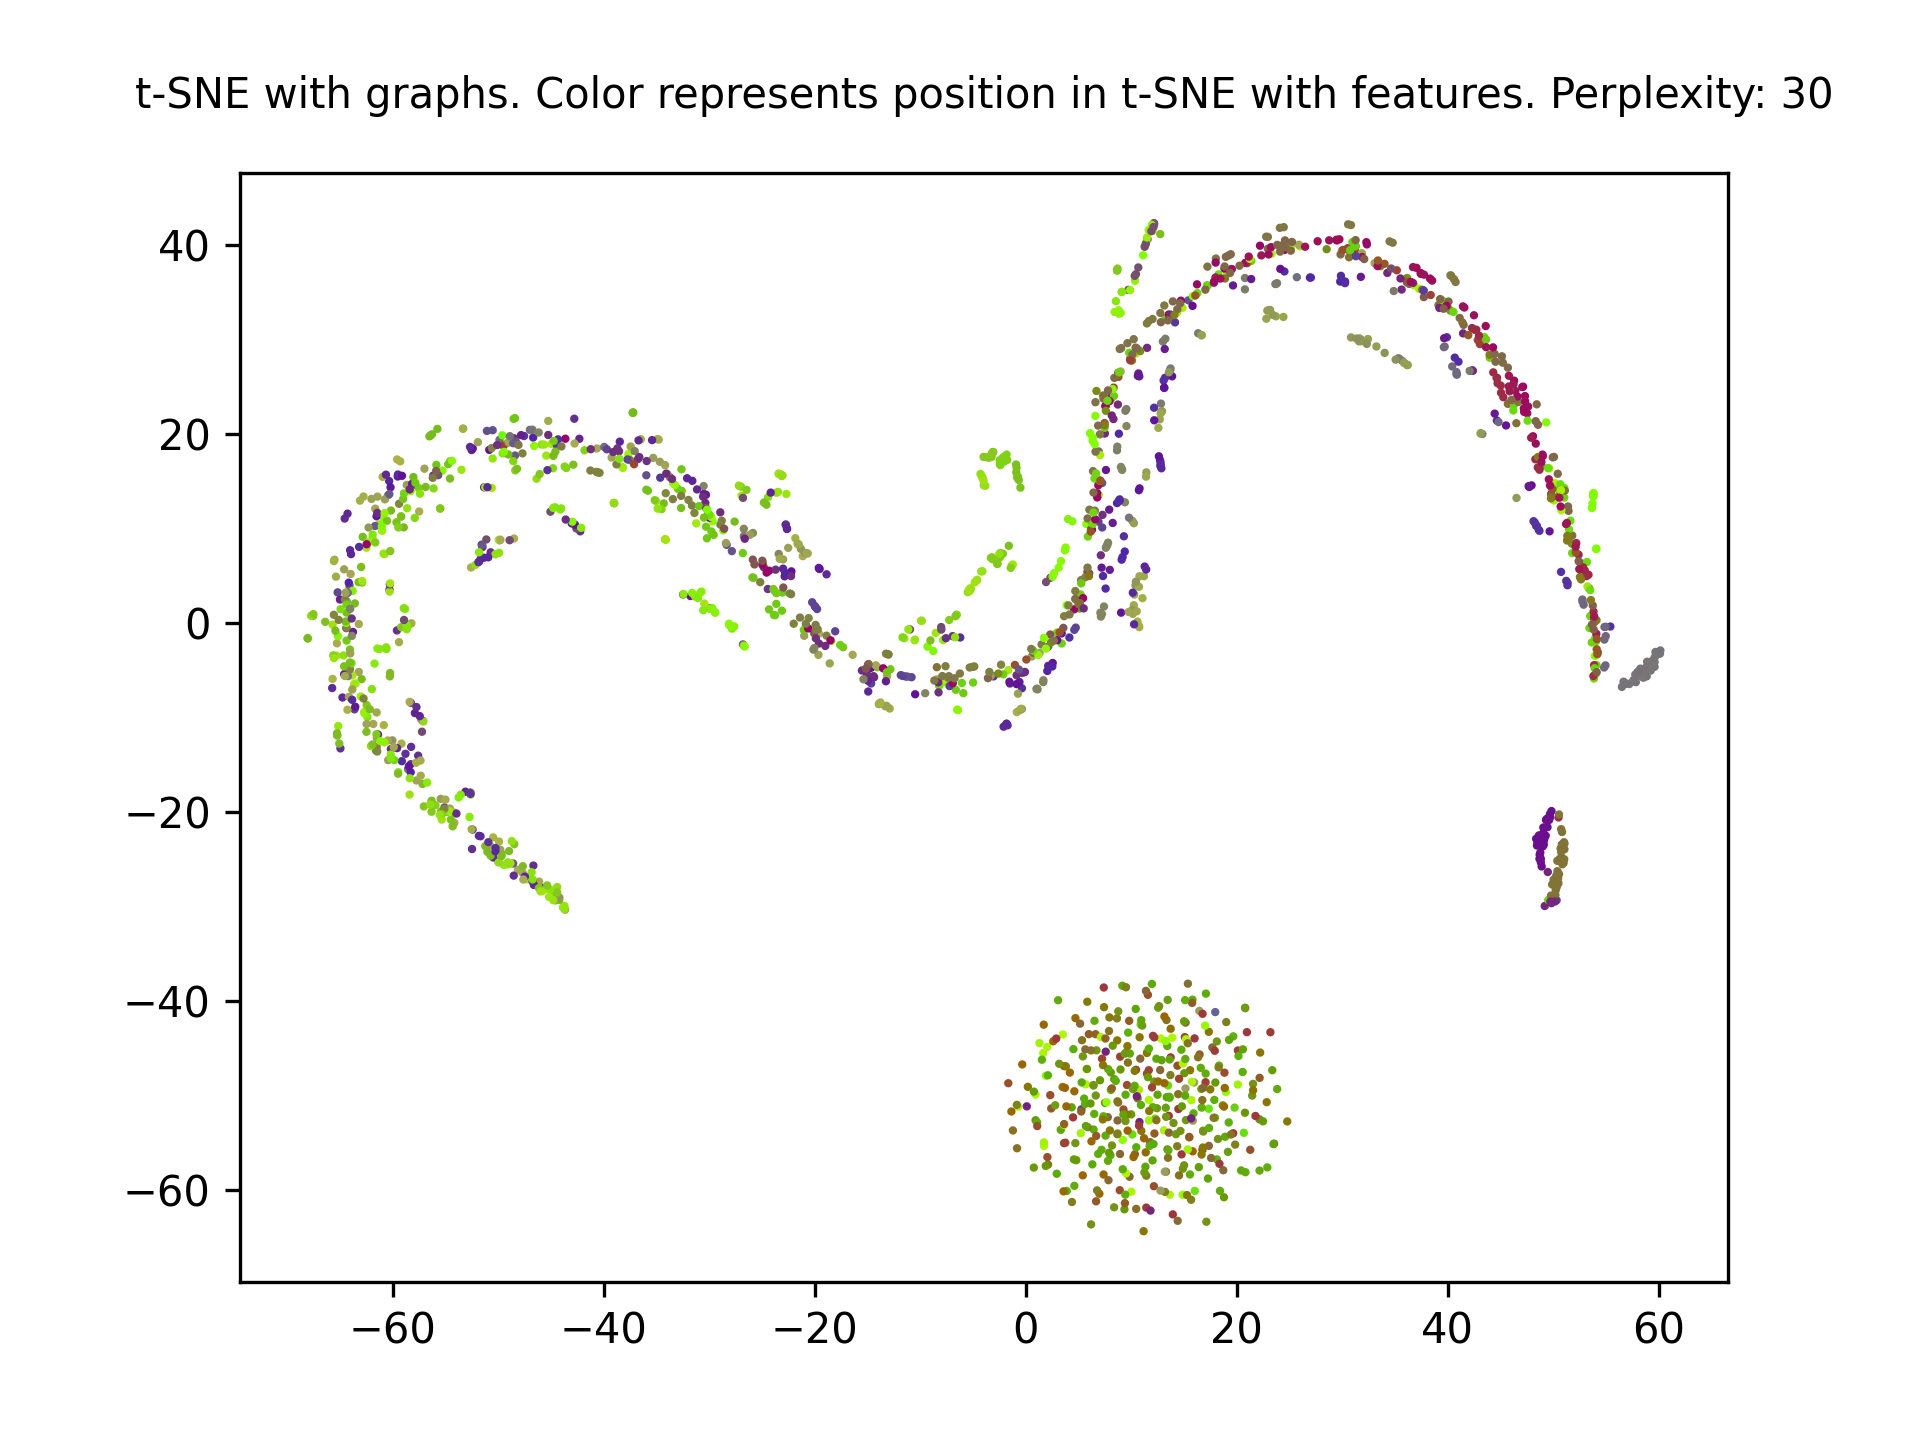
\includegraphics[width=0.45\textwidth]{images/tsne_gg_gl2vecAttr_graph_p30.png}
    }
    \qquad
    \subfloat[Point-Line\label{fig:tsne_pointad_graph}]{
        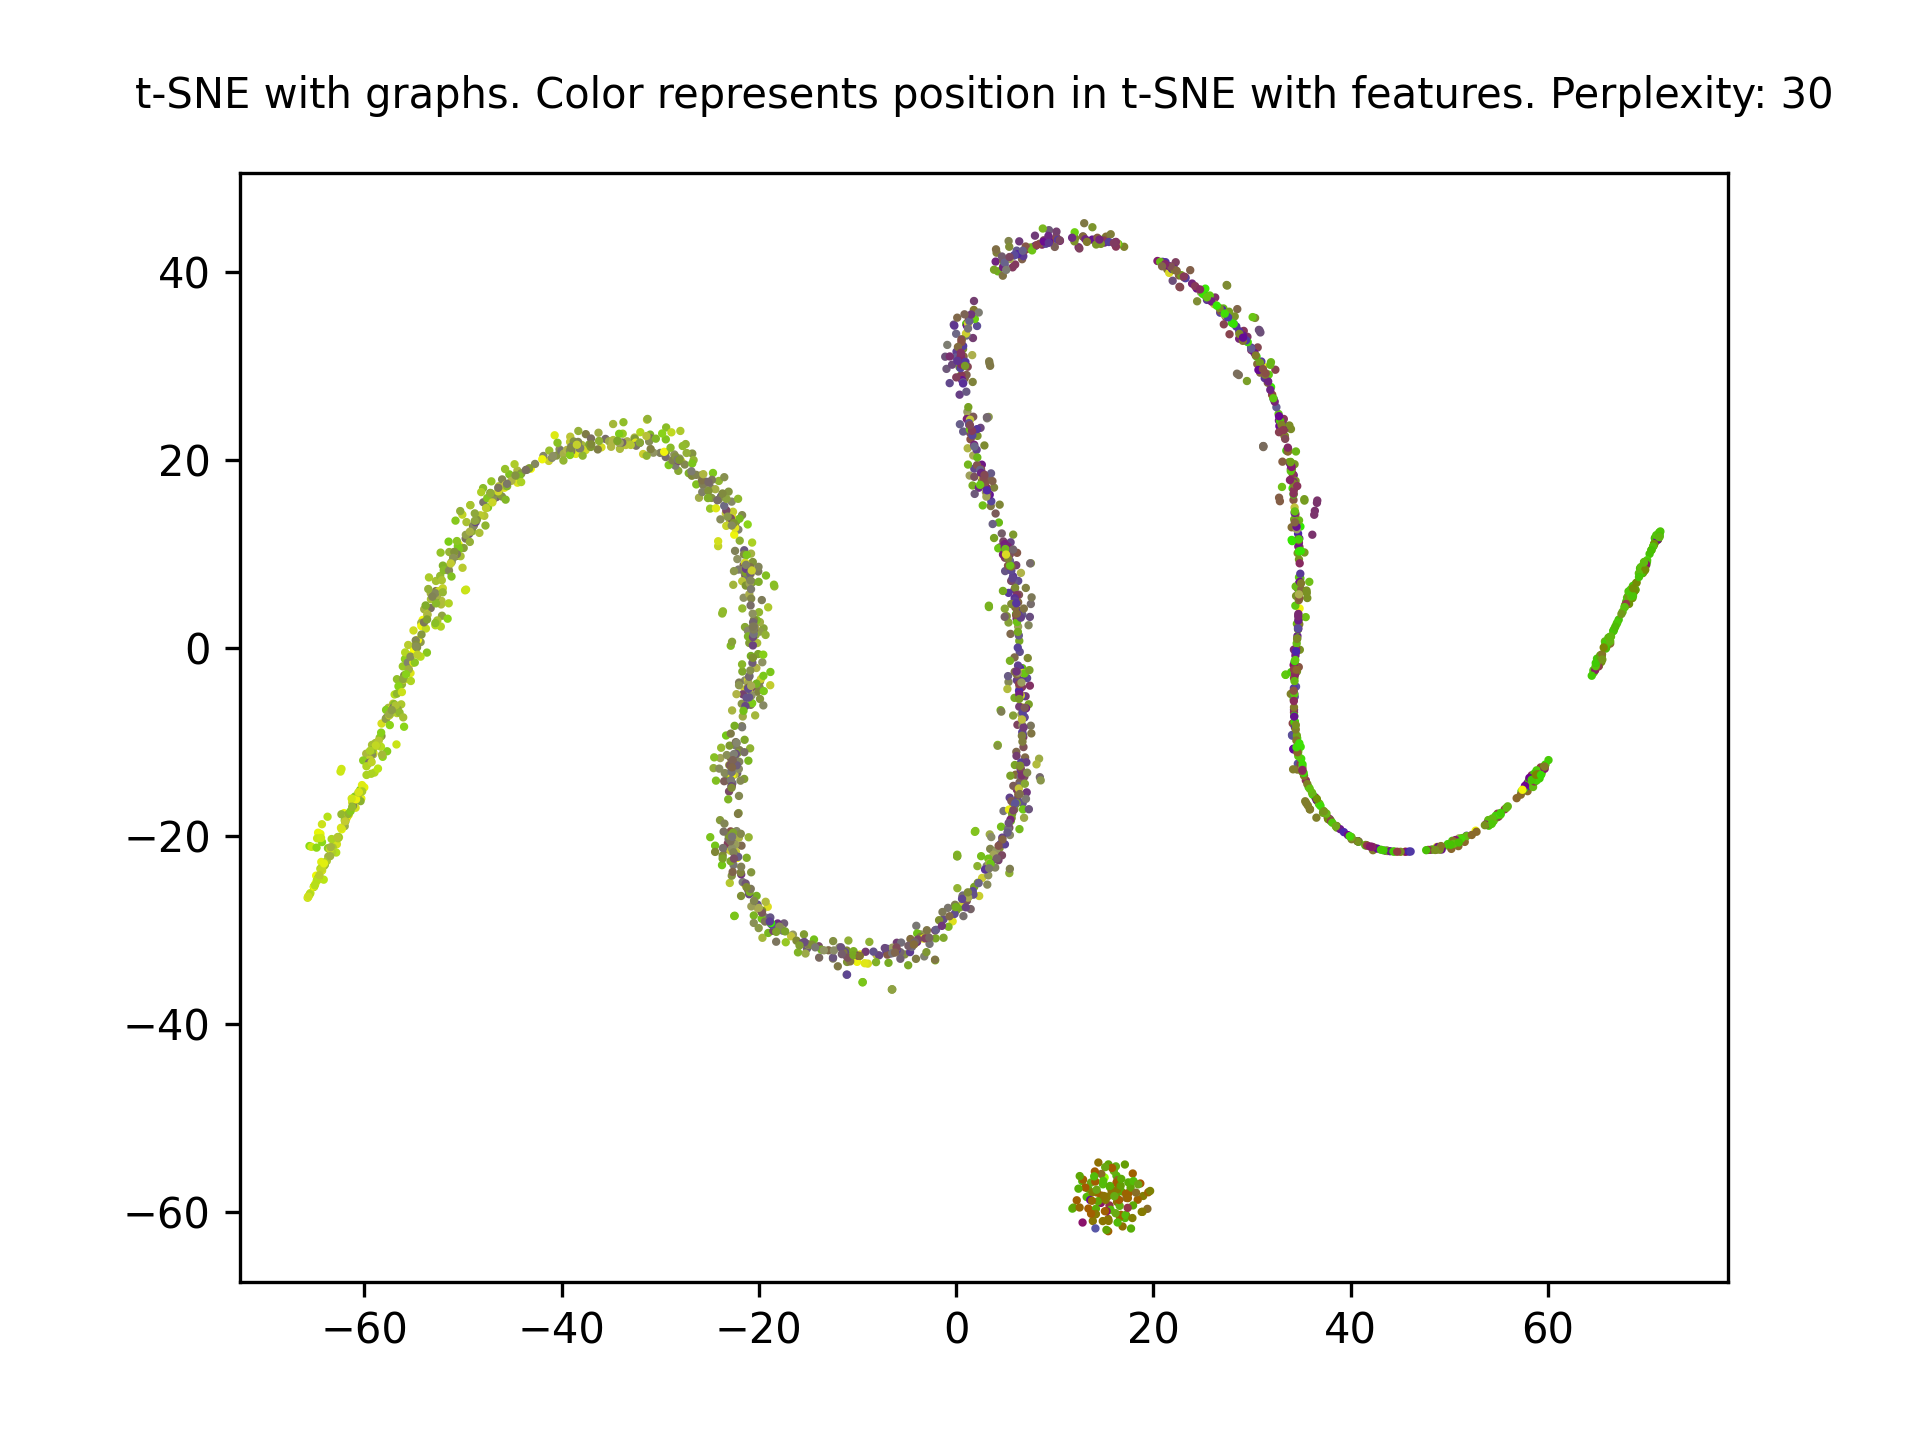
\includegraphics[width=0.45\textwidth]{images/tsne_pointad_gl2vecAttr_graph_p30.png}
    }
    \qquad
    \subfloat[SMT Genome\label{fig:tsne_smt_graph}]{
        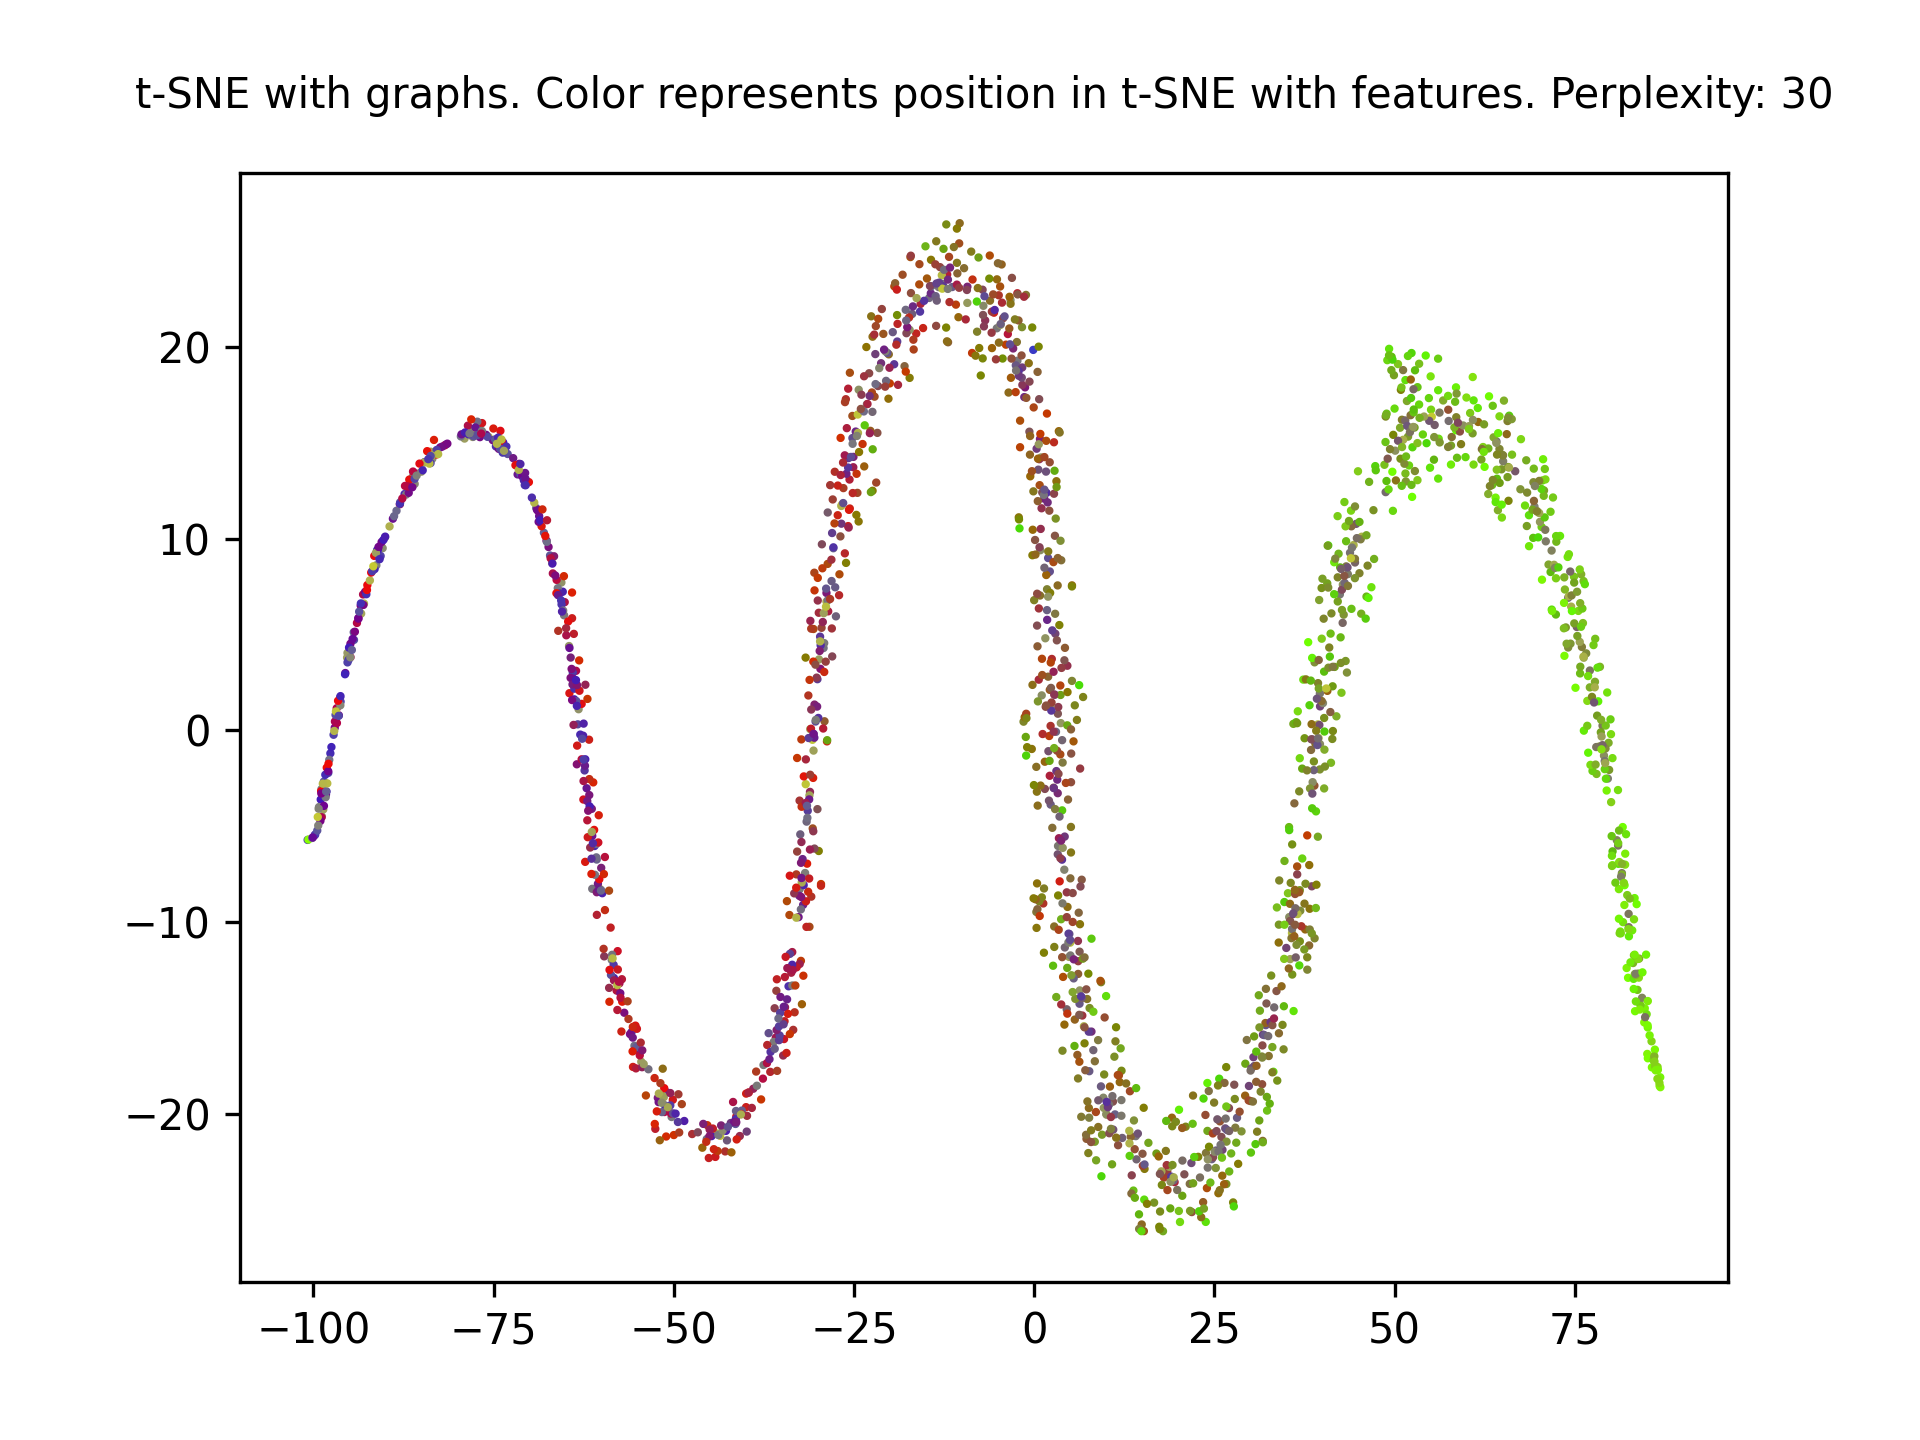
\includegraphics[width=0.45\textwidth]{images/tsne_smt_gl2vecAttr_graph_p30.png}
    }
    \qquad
    \caption{t-SNE analysis of the graphs for each genome representation.}
    \label{fig:tsne_graphs}
\end{figure}

As we did for the images, we have empirically examined the graphs corresponding to the points in the plot in order to ensure that graphs that have been placed close in the space projected by t-SNE are actually structurally similar graphs, and we include some examples in figure \cref{fig:tsne_graphs_examples}. We have observed that graphs, for all representations, are mostly placed on a continuum from simpler graphs all the way to more complex graphs. We also questioned if graph similarity was in any way related to the image similarity of the map. Empirically, it was not the case, and in figure \cref{fig:dist_graphs_images} we have plotted, for any two maps, the distance in the space projected by the image \textit{t-SNE} and the distance in the space projected by the graph \textit{t-SNE}. We have observed no correlation between the two distances, as expected.

\begin{figure}[hbt!]
    \centering
    \subfloat[-30, -56]{
        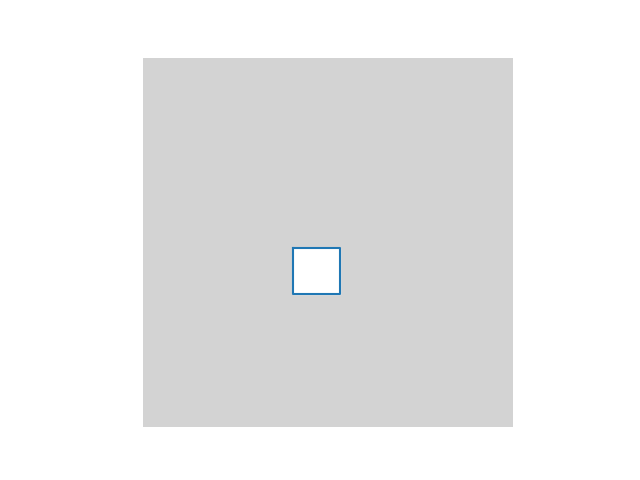
\includegraphics[width=0.22\textwidth]{images/tsne_samples/gr11.png}
        \includegraphics[width=0.22\textwidth]{images/tsne_samples/gr12.png}
    }
    \qquad
    \subfloat[-88, -6]{
        \includegraphics[width=0.22\textwidth]{images/tsne_samples/gr21.png}
        \includegraphics[width=0.22\textwidth]{images/tsne_samples/gr22.png}
    }
    \qquad
    \subfloat[-51, -17]{
        \includegraphics[width=0.22\textwidth]{images/tsne_samples/gr31.png}
        \includegraphics[width=0.22\textwidth]{images/tsne_samples/gr32.png}
    }
    \qquad
    \subfloat[-24, -20]{
        \includegraphics[width=0.22\textwidth]{images/tsne_samples/gr41.png}
        \includegraphics[width=0.22\textwidth]{images/tsne_samples/gr42.png}
    }
    \qquad
    \subfloat[12, 22]{
        \includegraphics[width=0.22\textwidth]{images/tsne_samples/gr51.png}
        \includegraphics[width=0.22\textwidth]{images/tsne_samples/gr52.png}
    }
    \qquad
    \subfloat[80, -4]{
        \includegraphics[width=0.22\textwidth]{images/tsne_samples/gr61.png}
        \includegraphics[width=0.22\textwidth]{images/tsne_samples/gr62.png}
    }
    \caption[t-SNE graph similarity examples]{Samples of random couples of points close in the space projected by \textit{t-SNE} for the All-Black representation, chosen to make an example. We report to the approximate location of each couple. Graphs are not as clearly similar, but we can see that the further along the x-axis we move, the more complex the graphs become (excluding the first example, which is the red cluster below the curve).}
    \label{fig:tsne_graphs_examples}
\end{figure}

\begin{figure}[hbt!]
    \centering
    \subfloat[All-black\label{fig:dist_graphs_images_ab}]{
        \includegraphics[width=0.45\textwidth]{images/tsne_ab_gl2vecAttr_disttsne_img_graph_tsne_ab_gl2vecAttr_p30.png}
    }
    \qquad
    \subfloat[Grid-Graph\label{fig:dist_graphs_images_gg}]{
        \includegraphics[width=0.45\textwidth]{images/tsne_gg_gl2vecAttr_disttsne_img_graph_tsne_gg_gl2vecAttr_p30.png}
    }
    \qquad
    \subfloat[Point-Line\label{fig:dist_graphs_images_pointad}]{
        \includegraphics[width=0.45\textwidth]{images/tsne_pointad_gl2vecAttr_disttsne_img_graph_tsne_pointad_gl2vecAttr_p30.png}
    }
    \qquad
    \subfloat[SMT Genome\label{fig:dist_graphs_images_smt}]{
        \includegraphics[width=0.45\textwidth]{images/tsne_smt_gl2vecAttr_disttsne_img_graph_tsne_smt_gl2vecAttr_p30.png}
    }
    \qquad
    \caption{Scatter plot of the distances in the image space and in the graph space.}
    \label{fig:dist_graphs_images}
\end{figure}

Regarding the result of \textit{t-SNE} itself (fig \cref{fig:tsne_graphs}) we notice that, instead of multiple clusters, we only have a couple, where one is shaped as a curve. Along this curve we can see a gradient of colors, which suggests that maps that are close in the \textit{t-SNE} space of the features are also close in the \textit{t-SNE} space of the graphs. This is an interesting result, as it suggests that the features we have extracted are indeed correlated with the topological structure of the maps.

To further investigate this correlation, like in the image case, we have plotted on a graph a point for each couple of maps, where the x-axis represents the distance in the \textit{t-SNE} space of the features and the y-axis represents the distance in the \textit{t-SNE} space of the graphs. The results are shown in figure \cref{fig:tsne_distance_graphs}.  

\begin{figure}[hbt!]
    \centering
    \subfloat[All-black\label{fig:tsne_ab_distance_graph}]{
        \includegraphics[width=0.45\textwidth]{images/tsne_ab_gl2vecAttr_disttsne_feat_graph_p30.png}
    }
    \qquad
    \subfloat[Grid-Graph\label{fig:tsne_gg_distance_graph}]{
        \includegraphics[width=0.45\textwidth]{images/tsne_gg_gl2vecAttr_disttsne_feat_graph_p30.png}
    }
    \qquad
    \subfloat[Point-Line\label{fig:tsne_pointad_distance_graph}]{
        \includegraphics[width=0.45\textwidth]{images/tsne_pointad_gl2vecAttr_disttsne_feat_graph_p30.png}
    }
    \qquad
    \subfloat[SMT Genome\label{fig:tsne_smt_distance_graph}]{
        \includegraphics[width=0.45\textwidth]{images/tsne_smt_gl2vecAttr_disttsne_feat_graph_p30.png}
    }
    \qquad
    \caption{Scatter plot of the distances in the feature space and in the graph space.}
    \label{fig:tsne_distance_graphs}
\end{figure}

\textit{All-Black} and \textit{Point-Line} representations show a clear correlation between the distances in the two spaces, while \textit{Grid-Graph} and \textit{SMT Genome} do not show as clear of a correlation. 

In order to specifically identify interesting features, we have then considered the features defined in \cref{sec:correlation_analysis}. For each feature, we plotted a graph where each point represents a couple of maps, with the x-axis representing the difference of the examined feature between the two maps and the y-axis representing the distance in the space of the graphs projected by \textit{t-SNE}. 

Not all feature showed a clear correlation, which explains the not-so-clear correlation in figure \cref{fig:tsne_distance_graphs} especially for the \textit{Grid-Graph} and \textit{SMT Genome} representations, but in figures \cref{fig:dist_feat_graph_ab}, \cref{fig:dist_feat_graph_gg}, \cref{fig:dist_feat_graph_point} and \cref{fig:dist_feat_graph_smt} we can see that some features do show a clear correlation with the distance in the \textit{t-SNE} space of the graphs. Among these, we highlight the \textit{area}, which correlated positively with a lot of features in \cref{sec:correlation_analysis}, and the \textit{maxSymmetry}, which correlates negatively with the \textit{area}. We highlight \textit{pace} and \textit{density}, which seem to be the only feature that shows a clear correlation with the distance in the \textit{t-SNE} space of the graphs for all representations. We also highlight \textit{averageEccentricity}, which is negatively correlated with \textit{pace}. Finally, we included \textit{averageMincut} and \textit{numberCyclesOneRoom}, even though their correlation with the distance is not so clear as the others, because we believe them to be interesting features, as they are related to the concept of "multiple paths" and are interesting metrics overall. 

We believe thus that these features are worth exploring using a QD approach, as these results suggest that illuminating these features may lead to discovering maps with varied topological structure.

\begin{figure}[hbt!]
    \centering
    \subfloat[area]{\includegraphics[width=0.15\textwidth]{images/distfeat/tsne_ab_gl2vecAttr_distfeat_graph_area_p30.jpg}}
    \qquad
    \subfloat[averageEccentricity]{\includegraphics[width=0.15\textwidth]{images/distfeat/tsne_ab_gl2vecAttr_distfeat_graph_averageEccentricity_p30.jpg}}
    \qquad
    \subfloat[averageLocalMaximaValuePercentVisibility]{\includegraphics[width=0.15\textwidth]{images/distfeat/tsne_ab_gl2vecAttr_distfeat_graph_averageLocalMaximaValuePercentVisibility_p30.jpg}}
    \qquad
    \subfloat[averageMincut]{\includegraphics[width=0.15\textwidth]{images/distfeat/tsne_ab_gl2vecAttr_distfeat_graph_averageMincut_p30.jpg}}
    \qquad
    \subfloat[averageRoomBetweenness]{\includegraphics[width=0.15\textwidth]{images/distfeat/tsne_ab_gl2vecAttr_distfeat_graph_averageRoomBetweenness_p30.jpg}}
    \qquad
    \subfloat[density]{\includegraphics[width=0.15\textwidth]{images/distfeat/tsne_ab_gl2vecAttr_distfeat_graph_density_p30.jpg}}
    \qquad
    \subfloat[maxSymmetry]{\includegraphics[width=0.15\textwidth]{images/distfeat/tsne_ab_gl2vecAttr_distfeat_graph_maxSymmetry_p30.jpg}}
    \qquad
    \subfloat[maxValuePosition]{\includegraphics[width=0.15\textwidth]{images/distfeat/tsne_ab_gl2vecAttr_distfeat_graph_maxValuePosition_p30.jpg}}
    \qquad
    \subfloat[numberCyclesOneRoom]{\includegraphics[width=0.15\textwidth]{images/distfeat/tsne_ab_gl2vecAttr_distfeat_graph_numberCyclesOneRoom_p30.jpg}}
    \qquad
    \subfloat[pace]{\includegraphics[width=0.15\textwidth]{images/distfeat/tsne_ab_gl2vecAttr_distfeat_graph_pace_p30.jpg}}
    \qquad
    \subfloat[peripheryPercent]{\includegraphics[width=0.15\textwidth]{images/distfeat/tsne_ab_gl2vecAttr_distfeat_graph_peripheryPercent_p30.jpg}}
    \qquad
    \subfloat[stdValuePercentVisibility]{\includegraphics[width=0.15\textwidth]{images/distfeat/tsne_ab_gl2vecAttr_distfeat_graph_stdValuePercentVisibility_p30.jpg}}
    \caption{Scatter plot of the difference of the feature and the distance in the \textit{t-SNE} of graphs for the \textit{All-Black} representation.}
    \label{fig:dist_feat_graph_ab}
\end{figure}
\begin{figure}[hbt!]
    \centering
    \subfloat[area]{\includegraphics[width=0.15\textwidth]{images/distfeat/tsne_gg_gl2vecAttr_distfeat_graph_area_p30.jpg}}
    \qquad
    \subfloat[averageEccentricity]{\includegraphics[width=0.15\textwidth]{images/distfeat/tsne_gg_gl2vecAttr_distfeat_graph_averageEccentricity_p30.jpg}}
    \qquad
    \subfloat[averageMincut]{\includegraphics[width=0.15\textwidth]{images/distfeat/tsne_gg_gl2vecAttr_distfeat_graph_averageMincut_p30.jpg}}
    \qquad
    \subfloat[density]{\includegraphics[width=0.15\textwidth]{images/distfeat/tsne_gg_gl2vecAttr_distfeat_graph_density_p30.jpg}}
    \qquad
    \subfloat[numberCyclesOneRoom]{\includegraphics[width=0.15\textwidth]{images/distfeat/tsne_gg_gl2vecAttr_distfeat_graph_numberCyclesOneRoom_p30.jpg}}
    \qquad
    \subfloat[pace]{\includegraphics[width=0.15\textwidth]{images/distfeat/tsne_gg_gl2vecAttr_distfeat_graph_pace_p30.jpg}}
    \qquad
    \subfloat[peripheryPercent]{\includegraphics[width=0.15\textwidth]{images/distfeat/tsne_gg_gl2vecAttr_distfeat_graph_peripheryPercent_p30.jpg}}
    \caption{Scatter plot of the difference of the feature and the distance in the \textit{t-SNE} of graphs for the \textit{Grid-Graph} representation.}
    \label{fig:dist_feat_graph_gg}
\end{figure}
\begin{figure}[hbt!]
    \centering
    \subfloat[area]{\includegraphics[width=0.15\textwidth]{images/distfeat/tsne_pointad_gl2vecAttr_distfeat_graph_area_p30.jpg}}
    \qquad
    \subfloat[averageEccentricity]{\includegraphics[width=0.15\textwidth]{images/distfeat/tsne_pointad_gl2vecAttr_distfeat_graph_averageEccentricity_p30.jpg}}
    \qquad
    \subfloat[averageLocalMaximaValuePercentVisibility]{\includegraphics[width=0.15\textwidth]{images/distfeat/tsne_pointad_gl2vecAttr_distfeat_graph_averageLocalMaximaValuePercentVisibility_p30.jpg}}
    \qquad
    \subfloat[averageMincut]{\includegraphics[width=0.15\textwidth]{images/distfeat/tsne_pointad_gl2vecAttr_distfeat_graph_averageMincut_p30.jpg}}
    \qquad
    \subfloat[averageRoomBetweenness]{\includegraphics[width=0.15\textwidth]{images/distfeat/tsne_pointad_gl2vecAttr_distfeat_graph_averageRoomBetweenness_p30.jpg}}
    \qquad
    \subfloat[density]{\includegraphics[width=0.15\textwidth]{images/distfeat/tsne_pointad_gl2vecAttr_distfeat_graph_density_p30.jpg}}
    \qquad
    \subfloat[entropy]{\includegraphics[width=0.15\textwidth]{images/distfeat/tsne_pointad_gl2vecAttr_distfeat_graph_entropy_p30.jpg}}
    \qquad
    \subfloat[maxSymmetry]{\includegraphics[width=0.15\textwidth]{images/distfeat/tsne_pointad_gl2vecAttr_distfeat_graph_maxSymmetry_p30.jpg}}
    \qquad
    \subfloat[maxTraces]{\includegraphics[width=0.15\textwidth]{images/distfeat/tsne_pointad_gl2vecAttr_distfeat_graph_maxTraces_p30.jpg}}
    \qquad
    \subfloat[maxValuePosition]{\includegraphics[width=0.15\textwidth]{images/distfeat/tsne_pointad_gl2vecAttr_distfeat_graph_maxValuePosition_p30.jpg}}
    \qquad
    \subfloat[maxValueVisibility]{\includegraphics[width=0.15\textwidth]{images/distfeat/tsne_pointad_gl2vecAttr_distfeat_graph_maxValueVisibility_p30.jpg}}
    \qquad
    \subfloat[pace]{\includegraphics[width=0.15\textwidth]{images/distfeat/tsne_pointad_gl2vecAttr_distfeat_graph_pace_p30.jpg}}
    \qquad
    \subfloat[numberCyclesOneRoom]{\includegraphics[width=0.15\textwidth]{images/distfeat/tsne_pointad_gl2vecAttr_distfeat_graph_numberCyclesOneRoom_p30.jpg}}
    \caption{Scatter plot of the difference of the feature and the distance in the \textit{t-SNE} of graphs for the \textit{Point-Line} representation.}
    \label{fig:dist_feat_graph_point}
\end{figure}
\begin{figure}[hbt!]
    \centering
    \subfloat[averageLocalMaximaValuePercentVisibility]{\includegraphics[width=0.15\textwidth]{images/distfeat/tsne_smt_gl2vecAttr_distfeat_graph_averageLocalMaximaValuePercentVisibility_p30.jpg}}
    \qquad
    \subfloat[averageMincut]{\includegraphics[width=0.15\textwidth]{images/distfeat/tsne_smt_gl2vecAttr_distfeat_graph_averageMincut_p30.jpg}}
    \qquad
    \subfloat[averageRoomBetweenness]{\includegraphics[width=0.15\textwidth]{images/distfeat/tsne_smt_gl2vecAttr_distfeat_graph_averageRoomBetweenness_p30.jpg}}
    \qquad
    \subfloat[density]{\includegraphics[width=0.15\textwidth]{images/distfeat/tsne_smt_gl2vecAttr_distfeat_graph_density_p30.jpg}}
    \qquad
    \subfloat[numberCyclesOneRoom]{\includegraphics[width=0.15\textwidth]{images/distfeat/tsne_smt_gl2vecAttr_distfeat_graph_numberCyclesOneRoom_p30.jpg}}
    \qquad
    \subfloat[pace]{\includegraphics[width=0.15\textwidth]{images/distfeat/tsne_smt_gl2vecAttr_distfeat_graph_pace_p30.jpg}}
    \caption{Scatter plot of the difference of the feature and the distance in the \textit{t-SNE} of graphs for the \textit{SMT Genome} representation.}
    \label{fig:dist_feat_graph_smt}
\end{figure}

\clearpage
\section{Experiments with MAP-Elites}
Using the insights gained by the analysis of the features' correlation and the \textit{t-SNE} analysis, we will now define some interesting \textit{behavioral features} to be used in a \textit{MAP-Elites} algorithm. 

Given that it would be unfeasible to guess a sensible range for each feature, and that we cannot know a priori the distribution of the features, we will employ the \textit{MAP-Elites with Sliding Boundaries} (MESB) algorithm, which is an extension of the original MAP-Elites algorithm that allows for the automatic adjustment of the archive's bins' boundaries according to the distribution of the features themselves \cite{fontaine_mapping_2019}. Our archive will hold 10 bins for each feature, for a total of 100 maximum solutions, which we found to be a good compromise between generating a good variety of maps and still being able to explore the archive in a reasonable number of iterations.

It's worth mentioning that we explored the possibility of using CMA-ME \cite{fontaine_covariance_2020}, but results were unsatisfactory, mainly due to the impossibility of defining ad-hoc mutation and crossover operators for the genomes, impeding the effective search of the feature space.

Each run of the algorithm will start with 20 random individuals, and will run for 400 iterations with 10 emitters, meaning each iteration will generate 10 new individuals. Each individual will be evaluated through 5 matches. Matches are simulated using two bots in the \textit{Duel} game-mode of \textit{Project Arena}. The resulting features from the 5 matches are averaged and used to place the individual in the \textit{MESB} archive. 

Experiments will be run using bots whose skill levels differ vastly, which is possible thanks to the configurable bots introduced by \citeauthor{bari_evolutionary-based_2023} in \textit{Project Arena}. The goal of the evolution is that of producing diverse maps where matches are on average balanced despite the skill gap between the two bots, which is an interesting objective according to the literature \cite{lanzi_evolving_2014} \cite{bari_evolutionary-based_2023}. The balance of a match is measured through the \textit{entropy} feature, as described in \cref{subsec:emergent_features}.

We will repeat each experiment on all four genomes in order to compare the results.

\subsection{area - maxSymmetry}
\label{subsec:exp1}
The first couple of features we explored are \textit{area} and \textit{maxSymmetry}, which sported an average negative correlation of -0.88 (see \cref{sec:correlation_analysis}) and have shown a clear correlation in the \textit{t-SNE} space of the graphs for all representations except for \textit{SMT-Genome} (see \cref{sec:tsne_analysis}).

For this experiment we have used a \textit{sniper} bot with a skill level of 0.15 and a \textit{shotgun} bot with a skill level of 0.85, searching for maps that are balanced despite the skill gap between the two bots.

The following figures will illustrate the heatmap of the archive obtained, the ccdf\footnote{Complementary cumulative distribution function} of the fitness of elites (in our case, the probability that a random elite will have a value of \textit{entropy} above a certain level), the QD score of the archive overtime (sum of entropy of all elites in the archive), the maximum value of entropy achieved in the archive over time, the size of the archive over time and the number of unfeasible individuals. 


\begin{figure}[H]
    \centering
    \subfloat[All-Black]{\includegraphics[width=0.45\textwidth]{images/Exp1/heatmap_ab.png}}
    \subfloat[Grid-Graph]{\includegraphics[width=0.45\textwidth]{images/Exp1/heatmap_gg.png}}
    \qquad
    \subfloat[Point-Line]{\includegraphics[width=0.45\textwidth]{images/Exp1/heatmap_pointad.png}}
    \subfloat[SMT-Genome]{\includegraphics[width=0.45\textwidth]{images/Exp1/heatmap_smt.png}}
    \caption{Heatmap of the archive obtained with the \textit{area} and \textit{maxSymmetry} features.}
    \label{fig:heatmap_exp1}
\end{figure}

From the heatmaps in figure \cref{fig:heatmap_exp1} it is immediately apparent that not all representations are able to generate the same range of maps. \textit{Grid-Graph} shows by far the most amount of symmetry, stemming from its nature of generating maps with a grid-like structure, but is unable to generate very asymmetrical maps, while \textit{All-Black} shows the opposite trend and \textit{Point-Line} shows the largest delta. Regarding the area, \textit{Point-Line} is again the one that can generate the most variety, having maps with up to 50\% of the area of the map walkable. All-Black and Grid-Graph generate smaller maps, but maps that are too small are rather uninteresting, if anything avoiding maps so small that only a single room is present is a good feature of a representation, as they are of little interest when considering actual maps that could be played by humans.

\begin{figure}[H]
    \centering
    \includegraphics[width=0.5\textwidth]{images/Exp1/archive_size.png}
    \caption{Size of the archive over time with the \textit{area} and \textit{maxSymmetry} features.}
    \label{fig:archive_size_exp1}
\end{figure} 

From figure \cref{fig:archive_size_exp1} we can see that the \textit{Grid-Graph} representation has the fewest elites in the archive, which again shows that it is limited in the amount of variety it can generate. \textit{All-Black} achieves slightly better results, followed by \textit{Point-Line} and then \textit{SMT-Genome}, which achieves the most elites in the archive. These results suggest that \textit{SMT-Genome} is able to generate more varied maps, but we should take into account that \textit{Point-Line} achieves similar results while being able to generate maps with a wider range for \textit{area} and \textit{maxSymmetry}.

\vspace*{\fill}
\begin{figure}[hbt!]
    \centering
    \includegraphics[width=0.5\textwidth]{images/Exp1/archive_ccdf.png}
    \caption{CCDF of the fitness of elites obtained with the \textit{area} and \textit{maxSymmetry} features.}
    \label{fig:ccdf_exp1}
\end{figure}


\begin{figure}[H]
    \centering
    \includegraphics[width=0.5\textwidth]{images/Exp1/qd_score.png}
    \caption{QD score of the archive obtained with the \textit{area} and \textit{maxSymmetry} features.}
    \label{fig:qd_score_exp1}
\end{figure}
\vspace*{\fill}


\begin{figure}[H]
    \centering
    \includegraphics[width=0.5\textwidth]{images/Exp1/max_score.png}
    \caption{Maximum value of entropy achieved in the archive over time with the \textit{area} and \textit{maxSymmetry} features.}
    \label{fig:max_score_exp1}
\end{figure}
\vspace*{\fill}


From figure \ref{fig:max_score_exp1} we gauge that \textit{Grid-Graph} and \textit{Point-Line} are able to achieve an almost perfect \textit{entropy} score of 1.0, while \textit{All-Black} and \textit{SMT-Genome} steadily improve their result without matching the other two representations. A likely reason for the difference in performance is the kind of maps these representations generate: \textit{All-Black} and \textit{SMT-Genome} struggle to create long corridors or large open spaces where a \textit{sniper} thrives, while \textit{Grid-Graph} and \textit{Point-Line} can generate such maps with ease. The ccdf of the fitness of elites in figure \cref{fig:ccdf_exp1} shows that \textit{Grid-Graph} achieves multiple maps with very high entropy, while Point-Line has a higher average entropy. Finally, \textit{Grid-Graph}, due to its under-full archive, has a lower QD score than the other representations, and \textit{All-Black} only barely surpasses it for the same reason, while the other two representations end up with a similar score, with \textit{SMT-Genome} having a slight edge over the others thanks to its fuller archive despite the lower average score of the elites (fig. \cref{fig:qd_score_exp1}). It is worth noting that \textit{SMT-Genome}'s QD score, although ultimately the highest, flattens out quickly when compared to the other representations, suggesting that this representation can quickly generate a good variety of good performing maps, but may struggle to improve them further.

It is worth remembering that, unlike the standard grid-like archive, the MESB archive has an archive with bins whose boundaries are recomputed periodically, which leads to the QD score having occasional dips when such re-computation causes some bins to merge, lowering the number of elites in the archive.


\begin{figure}[H]
    \centering
    \includegraphics[width=0.5\textwidth]{images/Exp1/failed.png}
    \caption{Number of unfeasible individuals over time with the \textit{area} and \textit{maxSymmetry} features.}
    \label{fig:failed_exp1}
\end{figure}

In figure \ref{fig:failed_exp1} we note how, as already stated in \cref{subsec:smt_genome}, roughly 160 \textit{SMT-Genome} individuals are unfeasible out of 4000, which amounts to \texttildelow 4\%. While this number is not negligible, we have seen how the \textit{SMT-Genome} still performs well even compared to \textit{All-Black}, and the archive is mostly full. We also note a couple of unfeasible individuals in the \textit{Point-Line} representation, which is likely the result of an error in the genotype-to-phenotype mapping when a map is mutated to have no rooms, but due to the extremely low number of unfeasible individuals we can safely disregard this issue.   

\subsubsection*{Analysis of maps in the archive}
As it is impossible to judge a map's quality solely based on its features, we will now show some examples of the best performing maps in the archive, taking care to show maps from distant bins in order to show and compare the variety of maps generated by the algorithm. We will show the maps, the traces of the bots and the visibility map for 4 maps for each genome in figures \cref{fig:best_maps_ab_exp1}, \cref{fig:best_maps_gg_exp1}, \cref{fig:best_maps_point_exp1} and \cref{fig:best_maps_smt_exp1}.

\begin{figure}[p]
    \centering
    \subfloat[Maps]{
        \includegraphics[width=0.22\textwidth]{images/Exp1/ab/map_2_1.png}
        \includegraphics[width=0.22\textwidth]{images/Exp1/ab/map_0_9.png}
        \includegraphics[width=0.22\textwidth]{images/Exp1/ab/map_9_0.png}
        \includegraphics[width=0.22\textwidth]{images/Exp1/ab/map_9_4.png}
    }
    \qquad
    \subfloat[Sniper traces]{
        \includegraphics[width=0.22\textwidth]{images/Exp1/ab/map_2_1_kill_traces_bot_0.png}
        \includegraphics[width=0.22\textwidth]{images/Exp1/ab/map_0_9_kill_traces_bot_0.png}
        \includegraphics[width=0.22\textwidth]{images/Exp1/ab/map_9_0_kill_traces_bot_0.png}
        \includegraphics[width=0.22\textwidth]{images/Exp1/ab/map_9_4_kill_traces_bot_0.png}
    }
    \qquad
    \subfloat[Shotgun traces]{
        \includegraphics[width=0.22\textwidth]{images/Exp1/ab/map_2_1_kill_traces_bot_1.png}
        \includegraphics[width=0.22\textwidth]{images/Exp1/ab/map_0_9_kill_traces_bot_1.png}
        \includegraphics[width=0.22\textwidth]{images/Exp1/ab/map_9_0_kill_traces_bot_1.png}
        \includegraphics[width=0.22\textwidth]{images/Exp1/ab/map_9_4_kill_traces_bot_1.png}
    }
    \qquad
    \subfloat[Visibility]{
        \includegraphics[width=0.22\textwidth]{images/Exp1/ab/visibility_map_2_1.png}
        \includegraphics[width=0.22\textwidth]{images/Exp1/ab/visibility_map_0_9.png}
        \includegraphics[width=0.22\textwidth]{images/Exp1/ab/visibility_map_9_0.png}
        \includegraphics[width=0.22\textwidth]{images/Exp1/ab/visibility_map_9_4.png}
    }
    \caption{Best performing \textit{All-Black} maps in the archive obtained with the \textit{area} and \textit{maxSymmetry} features.}
    \label{fig:best_maps_ab_exp1}
\end{figure}

\begin{figure}[p]
    \centering
    \subfloat[Maps]{
        \includegraphics[width=0.22\textwidth]{images/Exp1/gg/map_2_4.png}
        \includegraphics[width=0.22\textwidth]{images/Exp1/gg/map_3_6.png}
        \includegraphics[width=0.22\textwidth]{images/Exp1/gg/map_9_0.png}
        \includegraphics[width=0.22\textwidth]{images/Exp1/gg/map_9_5.png}
    }
    \qquad
    \subfloat[Sniper traces]{
        \includegraphics[width=0.22\textwidth]{images/Exp1/gg/map_2_4_kill_traces_bot_0.png}
        \includegraphics[width=0.22\textwidth]{images/Exp1/gg/map_3_6_kill_traces_bot_0.png}
        \includegraphics[width=0.22\textwidth]{images/Exp1/gg/map_9_0_kill_traces_bot_0.png}
        \includegraphics[width=0.22\textwidth]{images/Exp1/gg/map_9_5_kill_traces_bot_0.png}
    }
    \qquad
    \subfloat[Shotgun traces]{
        \includegraphics[width=0.22\textwidth]{images/Exp1/gg/map_2_4_kill_traces_bot_1.png}
        \includegraphics[width=0.22\textwidth]{images/Exp1/gg/map_3_6_kill_traces_bot_1.png}
        \includegraphics[width=0.22\textwidth]{images/Exp1/gg/map_9_0_kill_traces_bot_1.png}
        \includegraphics[width=0.22\textwidth]{images/Exp1/gg/map_9_5_kill_traces_bot_1.png}
    }
    \qquad
    \subfloat[Visibility]{
        \includegraphics[width=0.22\textwidth]{images/Exp1/gg/visibility_map_2_4.png}
        \includegraphics[width=0.22\textwidth]{images/Exp1/gg/visibility_map_3_6.png}
        \includegraphics[width=0.22\textwidth]{images/Exp1/gg/visibility_map_9_0.png}
        \includegraphics[width=0.22\textwidth]{images/Exp1/gg/visibility_map_9_5.png}
    }
    \caption{Best performing \textit{Grid-Graph} maps in the archive obtained with the \textit{area} and \textit{maxSymmetry} features.}
    \label{fig:best_maps_gg_exp1}
\end{figure}


\begin{figure}[p]
    \centering
    \subfloat[Maps]{
        \includegraphics[width=0.22\textwidth]{images/Exp1/point/map_4_2.png}
        \includegraphics[width=0.22\textwidth]{images/Exp1/point/map_0_9.png}
        \includegraphics[width=0.22\textwidth]{images/Exp1/point/map_9_0.png}
        \includegraphics[width=0.22\textwidth]{images/Exp1/point/map_8_7.png}
    }
    \qquad
    \subfloat[Sniper traces]{
        \includegraphics[width=0.22\textwidth]{images/Exp1/point/map_4_2_kill_traces_bot_0.png}
        \includegraphics[width=0.22\textwidth]{images/Exp1/point/map_0_9_kill_traces_bot_0.png}
        \includegraphics[width=0.22\textwidth]{images/Exp1/point/map_9_0_kill_traces_bot_0.png}
        \includegraphics[width=0.22\textwidth]{images/Exp1/point/map_8_7_kill_traces_bot_0.png}
    }
    \qquad
    \subfloat[Shotgun traces]{
        \includegraphics[width=0.22\textwidth]{images/Exp1/point/map_4_2_kill_traces_bot_1.png}
        \includegraphics[width=0.22\textwidth]{images/Exp1/point/map_0_9_kill_traces_bot_1.png}
        \includegraphics[width=0.22\textwidth]{images/Exp1/point/map_9_0_kill_traces_bot_1.png}
        \includegraphics[width=0.22\textwidth]{images/Exp1/point/map_8_7_kill_traces_bot_1.png}
    }
    \qquad
    \subfloat[Visibility]{
        \includegraphics[width=0.22\textwidth]{images/Exp1/point/visibility_map_4_2.png}
        \includegraphics[width=0.22\textwidth]{images/Exp1/point/visibility_map_0_9.png}
        \includegraphics[width=0.22\textwidth]{images/Exp1/point/visibility_map_9_0.png}
        \includegraphics[width=0.22\textwidth]{images/Exp1/point/visibility_map_8_7.png}
    }
    \caption{Best performing \textit{Point-Line} maps in the archive obtained with the \textit{area} and \textit{maxSymmetry} features.}
    \label{fig:best_maps_point_exp1}
\end{figure}


\begin{figure}[p]
    \centering
    \subfloat[Maps]{
        \includegraphics[width=0.22\textwidth]{images/Exp1/smt/map_2_5.png}
        \includegraphics[width=0.22\textwidth]{images/Exp1/smt/map_0_8.png}
        \includegraphics[width=0.22\textwidth]{images/Exp1/smt/map_9_0.png}
        \includegraphics[width=0.22\textwidth]{images/Exp1/smt/map_9_8.png}
    }
    \qquad
    \subfloat[Sniper traces]{
        \includegraphics[width=0.22\textwidth]{images/Exp1/smt/map_2_5_kill_traces_bot_0.png}
        \includegraphics[width=0.22\textwidth]{images/Exp1/smt/map_0_8_kill_traces_bot_0.png}
        \includegraphics[width=0.22\textwidth]{images/Exp1/smt/map_9_0_kill_traces_bot_0.png}
        \includegraphics[width=0.22\textwidth]{images/Exp1/smt/map_9_8_kill_traces_bot_0.png}
    }
    \qquad
    \subfloat[Shotgun traces]{
        \includegraphics[width=0.22\textwidth]{images/Exp1/smt/map_2_5_kill_traces_bot_1.png}
        \includegraphics[width=0.22\textwidth]{images/Exp1/smt/map_0_8_kill_traces_bot_1.png}
        \includegraphics[width=0.22\textwidth]{images/Exp1/smt/map_9_0_kill_traces_bot_1.png}
        \includegraphics[width=0.22\textwidth]{images/Exp1/smt/map_9_8_kill_traces_bot_1.png}
    }
    \qquad
    \subfloat[Visibility]{
        \includegraphics[width=0.22\textwidth]{images/Exp1/smt/visibility_map_2_5.png}
        \includegraphics[width=0.22\textwidth]{images/Exp1/smt/visibility_map_0_8.png}
        \includegraphics[width=0.22\textwidth]{images/Exp1/smt/visibility_map_9_0.png}
        \includegraphics[width=0.22\textwidth]{images/Exp1/smt/visibility_map_9_8.png}
    }
    \caption{Best performing \textit{SMT-Genome} maps in the archive obtained with the \textit{area} and \textit{maxSymmetry} features.}
    \label{fig:best_maps_smt_exp1}
\end{figure}

All representations generate maps with large open spaces or long narrow corridors. Snipers tend to achieve an advantage when they are positioned at the edge of a map and are able to gain good visibility over the majority of the map.

When seeing the kind of maps that perform close to the best in \textit{Grid-Graph} (fig. \ref{fig:best_maps_gg_exp1}) and in \textit{Point-Line} (fig. \ref{fig:best_maps_point_exp1}), we notice that dead ends and chokepoints are cut to a minimum, and when those are present (third map in \ref{fig:best_maps_point_exp1} shows a couple of short corridors that act as chokepoints) it is more likely that the shotgun makes use of them rather than the sniper. So, it stands to reason that \textit{All-Black} maps struggle to perform as well, since the maps' layouts are always very noisy with many dead-ends, sort corridors and sharp turns. In any case, the differences between maps with different features' values are clearly noticeable in the different topologies, as we would have expected from the \textit{t-SNE} analysis in \cref{subsec:tsne_graphs}. The two representations where the difference is less noticeable are \textit{Grid-Graph}, which was expected given the low correlation that resulted in our analysis, and \textit{SMT-Genome}, which is also expected as it showed no correlation with these two features in the same analysis (\cref{subsec:tsne_graphs}).

Despite performing well in terms of fitness, \textit{Grid-Graph} produces very dull maps, which are all comprised of one big room or a long corridor. Its difficulty in exploring the feature space was already an indication that maps were similar, but even the elites found in different niches are unable to show significant differences. When compared to \textit{Point-Line} and \textit{SMT-Genome}, which also performs well, layouts are more varied, with some alternate paths and covers, while still not being as noisy as \textit{All-Black} maps.

\clearpage

\subsection{pace - averageEccentricity}
\label{subsec:exp2}
The second experiment we will run is with the \textit{pace} and \textit{averageEccentricity} features, which showed a negative correlation of -0.79 (see \cref{sec:correlation_analysis}) and have shown a clear correlation in the \textit{t-SNE} space of the graphs.

For this experiment we have also used a \textit{sniper} bot with a skill level of 0.15 and a \textit{shotgun} bot with a skill level of 0.85, searching for maps that are balanced despite the skill gap between the two bots.

We present the same figures as in the previous experiment, which are the heatmap of the archive obtained, the ccdf of the fitness of elites, the QD score of the archive overtime, the maximum value of entropy achieved in the archive over time, the size of the archive over time and the number of unfeasible individuals. 

\begin{figure}[H]
    \centering
    \subfloat[All-Black]{\includegraphics[width=0.45\textwidth]{images/Exp2/heatmap_ab.png}}
    \subfloat[Grid-Graph]{\includegraphics[width=0.45\textwidth]{images/Exp2/heatmap_gg.png}}
    \qquad
    \subfloat[Point-Line]{\includegraphics[width=0.45\textwidth]{images/Exp2/heatmap_pointad.png}}
    \subfloat[SMT-Genome]{\includegraphics[width=0.45\textwidth]{images/Exp2/heatmap_smt.png}}
    \caption{Heatmap of the archive obtained with the \textit{pace} and \textit{averageEccentricity} features.}
    \label{fig:heatmap_exp2}
\end{figure}

From figure \ref{fig:heatmap_exp2} we see that all representations explore roughly the same range in both \textit{pace} and \textit{averageEccentricity}. The only noteworthy difference is that \textit{Grid-Graph} is able to achieve lower \textit{averageEccentricity} values, suggesting that it is able to generate maps with a more centralized layout, while \textit{SMT-Genome} is unable to achieve \textit{averageEccentricity} values above 120, suggesting that it is unable to generate maps with a layout too sparse. \textit{Grid-Graph} is instead able to generate maps with high \textit{pace} values, but despite this, we see fewer points in that part of the space when compared with \textit{Point-Line} and \textit{All-Black}, meaning that they are harder to generate and explore. In general, points are scattered in a sparser manner for \textit{Grid-Graph}, which suggests again the hardness of the illumination.

\begin{figure}[H]
    \centering
    \includegraphics[width=0.5\textwidth]{images/Exp2/archive_size.png}
    \caption{Size of the archive over time with the \textit{pace} and \textit{averageEccentricity} features.}
    \label{fig:archive_size_exp2}
\end{figure}

As in the previous experiment (\ref{subsec:exp1}), in figure \ref{fig:archive_size_exp2} we observe the \textit{Grid-Graph} representation has the fewest elites in the archive, which once again shows that it is limited in the amount of variety it can generate. Here \textit{ALL-Black}, \textit{Point-Line} and \textit{SMT-Genome} instead fill the archive similarly, although \textit{SMT-Genome} is faster in doing so, as also noted in the previous experiment. 

\begin{figure}[H]
    \centering
    \includegraphics[width=0.5\textwidth]{images/Exp2/archive_ccdf.png}
    \caption{CCDF of the fitness of elites obtained with the \textit{pace} and \textit{averageEccentricity} features.}
    \label{fig:ccdf_exp2}
\end{figure}

\begin{figure}[H]
    \centering
    \includegraphics[width=0.5\textwidth]{images/Exp2/qd_score.png}
    \caption{QD score of the archive obtained with the \textit{pace} and \textit{averageEccentricity} features.}
    \label{fig:qd_score_exp2}
\end{figure}

\begin{figure}[H]
    \centering
    \includegraphics[width=0.5\textwidth]{images/Exp2/max_score.png}
    \caption{Maximum value of entropy achieved in the archive over time with the \textit{pace} and \textit{averageEccentricity} features.}
    \label{fig:max_score_exp2}
\end{figure}

The distribution of the fitness of elites (figure \ref{fig:ccdf_exp2}) and the maximum fitness value achieved (figure \ref{fig:max_score_exp2}) shows similar results to our first experiment (\ref{subsec:exp1}), showing that \textit{Grid-Graph} and \textit{Point-Line} are able to achieve higher entropy values both on average and in the best maps, while \textit{All-Black} and \textit{SMT-Genome} similarly lag behind. The QD score (figure \ref{fig:qd_score_exp2}) shows that \textit{Grid-Graph} severely under-performs due to its under-filled archive, while the other representations boast similar scores, with \textit{SMT-Genome}. It is worth mentioning again that both here and in the previous experiment \textit{SMT-Genome}, while performing similarly at the end, shows a slightly different curve, reaching its maximum score faster than the other representations but being mostly flat afterwards, which brings about the same considerations as before. Here, however, \textit{SMT-Genome} does not end up scoring the highest, which further suggests that it may struggle to improve the maps it generates.

\begin{figure}[H]
    \centering
    \includegraphics[width=0.5\textwidth]{images/Exp2/failed.png}
    \caption{Number of unfeasible individuals over time with the \textit{pace} and \textit{averageEccentricity} features.}
    \label{fig:failed_exp2}
\end{figure}

In figure \ref{fig:failed_exp2} we see that the number of unfeasible individuals is roughly the same for \textit{SMT-Genome}, albeit a bit lower at 140, as in the previous experiment. This number is still not negligible, but the archive is mostly full, and the representation performs well. Moreover, the number of unfeasible individuals being consistent across experiments suggests that this metric is not tied to the features illuminated.

\subsubsection*{Analysis of maps in the archive}
As we did in the previous experiment, we will now show some examples of the best performing maps in the archive, taking care to show maps from distant bins in order to show and compare the variety of maps generated by the algorithm. Since the maps are generated with the same bots as in the previous experiment, we will also compare the designs produced to see whether illuminating different features has an impact on the kind of maps generated despite optimizing for the same objective. We will show the maps, the traces of the bots and the visibility map for 4 maps for each genome in figures \cref{fig:best_maps_ab_exp2}, \cref{fig:best_maps_gg_exp2}, \cref{fig:best_maps_point_exp2} and \cref{fig:best_maps_smt_exp2}.

\begin{figure}[p]
    \centering
    \subfloat[Maps]{
        \includegraphics[width=0.22\textwidth]{images/Exp2/ab/map_4_0.png}
        \includegraphics[width=0.22\textwidth]{images/Exp2/ab/map_0_6.png}
        \includegraphics[width=0.22\textwidth]{images/Exp2/ab/map_9_0.png}
        \includegraphics[width=0.22\textwidth]{images/Exp2/ab/map_9_7.png}
    }
    \qquad
    \subfloat[Sniper traces]{
        \includegraphics[width=0.22\textwidth]{images/Exp2/ab/map_4_0_kill_traces_bot_0.png}
        \includegraphics[width=0.22\textwidth]{images/Exp2/ab/map_0_6_kill_traces_bot_0.png}
        \includegraphics[width=0.22\textwidth]{images/Exp2/ab/map_9_0_kill_traces_bot_0.png}
        \includegraphics[width=0.22\textwidth]{images/Exp2/ab/map_9_7_kill_traces_bot_0.png}
    }
    \qquad
    \subfloat[Shotgun traces]{
        \includegraphics[width=0.22\textwidth]{images/Exp2/ab/map_4_0_kill_traces_bot_1.png}
        \includegraphics[width=0.22\textwidth]{images/Exp2/ab/map_0_6_kill_traces_bot_1.png}
        \includegraphics[width=0.22\textwidth]{images/Exp2/ab/map_9_0_kill_traces_bot_1.png}
        \includegraphics[width=0.22\textwidth]{images/Exp2/ab/map_9_7_kill_traces_bot_1.png}
    }
    \qquad
    \subfloat[Visibility]{
        \includegraphics[width=0.22\textwidth]{images/Exp2/ab/visibility_map_4_0.png}
        \includegraphics[width=0.22\textwidth]{images/Exp2/ab/visibility_map_0_6.png}
        \includegraphics[width=0.22\textwidth]{images/Exp2/ab/visibility_map_9_0.png}
        \includegraphics[width=0.22\textwidth]{images/Exp2/ab/visibility_map_9_7.png}
    }
    \caption{Best performing \textit{All-Black} maps in the archive obtained with the \textit{pace} and \textit{averageEccentricity} features.}
    \label{fig:best_maps_ab_exp2}
\end{figure}

\begin{figure}[p]
    \centering
    \subfloat[Maps]{
        \includegraphics[width=0.22\textwidth]{images/Exp2/gg/map_0_4.png}
        \includegraphics[width=0.22\textwidth]{images/Exp2/gg/map_2_9.png}
        \includegraphics[width=0.22\textwidth]{images/Exp2/gg/map_8_3.png}
        \includegraphics[width=0.22\textwidth]{images/Exp2/gg/map_4_7.png}
    }
    \qquad
    \subfloat[Sniper traces]{
        \includegraphics[width=0.22\textwidth]{images/Exp2/gg/map_0_4_kill_traces_bot_0.png}
        \includegraphics[width=0.22\textwidth]{images/Exp2/gg/map_2_9_kill_traces_bot_0.png}
        \includegraphics[width=0.22\textwidth]{images/Exp2/gg/map_8_3_kill_traces_bot_0.png}
        \includegraphics[width=0.22\textwidth]{images/Exp2/gg/map_4_7_kill_traces_bot_0.png}
    }
    \qquad
    \subfloat[Shotgun traces]{
        \includegraphics[width=0.22\textwidth]{images/Exp2/gg/map_0_4_kill_traces_bot_1.png}
        \includegraphics[width=0.22\textwidth]{images/Exp2/gg/map_2_9_kill_traces_bot_1.png}
        \includegraphics[width=0.22\textwidth]{images/Exp2/gg/map_8_3_kill_traces_bot_1.png}
        \includegraphics[width=0.22\textwidth]{images/Exp2/gg/map_4_7_kill_traces_bot_1.png}
    }
    \qquad
    \subfloat[Visibility]{
        \includegraphics[width=0.22\textwidth]{images/Exp2/gg/visibility_map_0_4.png}
        \includegraphics[width=0.22\textwidth]{images/Exp2/gg/visibility_map_2_9.png}
        \includegraphics[width=0.22\textwidth]{images/Exp2/gg/visibility_map_8_3.png}
        \includegraphics[width=0.22\textwidth]{images/Exp2/gg/visibility_map_4_7.png}
    }
    \caption{Best performing \textit{Grid-Graph} maps in the archive obtained with the \textit{pace} and \textit{averageEccentricity} features.}
    \label{fig:best_maps_gg_exp2}
\end{figure}

\begin{figure}[p]
    \centering
    \subfloat[Maps]{
        \includegraphics[width=0.22\textwidth]{images/Exp2/point/map_0_1.png}
        \includegraphics[width=0.22\textwidth]{images/Exp2/point/map_1_8.png}
        \includegraphics[width=0.22\textwidth]{images/Exp2/point/map_8_1.png}
        \includegraphics[width=0.22\textwidth]{images/Exp2/point/map_8_8.png}
    }
    \qquad
    \subfloat[Sniper traces]{
        \includegraphics[width=0.22\textwidth]{images/Exp2/point/map_0_1_kill_traces_bot_0.png}
        \includegraphics[width=0.22\textwidth]{images/Exp2/point/map_1_8_kill_traces_bot_0.png}
        \includegraphics[width=0.22\textwidth]{images/Exp2/point/map_8_1_kill_traces_bot_0.png}
        \includegraphics[width=0.22\textwidth]{images/Exp2/point/map_8_8_kill_traces_bot_0.png}
    }
    \qquad
    \subfloat[Shotgun traces]{
        \includegraphics[width=0.22\textwidth]{images/Exp2/point/map_0_1_kill_traces_bot_1.png}
        \includegraphics[width=0.22\textwidth]{images/Exp2/point/map_1_8_kill_traces_bot_1.png}
        \includegraphics[width=0.22\textwidth]{images/Exp2/point/map_8_1_kill_traces_bot_1.png}
        \includegraphics[width=0.22\textwidth]{images/Exp2/point/map_8_8_kill_traces_bot_1.png}
    }
    \qquad
    \subfloat[Visibility]{
        \includegraphics[width=0.22\textwidth]{images/Exp2/point/visibility_map_0_1.png}
        \includegraphics[width=0.22\textwidth]{images/Exp2/point/visibility_map_1_8.png}
        \includegraphics[width=0.22\textwidth]{images/Exp2/point/visibility_map_8_1.png}
        \includegraphics[width=0.22\textwidth]{images/Exp2/point/visibility_map_8_8.png}
    }
    \caption{Best performing \textit{Point-Line} maps in the archive obtained with the \textit{pace} and \textit{averageEccentricity} features.}
    \label{fig:best_maps_point_exp2}
\end{figure}

\begin{figure}[p]
    \centering
    \subfloat[Maps]{
        \includegraphics[width=0.22\textwidth]{images/Exp2/smt/map_0_2.png}
        \includegraphics[width=0.22\textwidth]{images/Exp2/smt/map_2_8.png}
        \includegraphics[width=0.22\textwidth]{images/Exp2/smt/map_9_0.png}
        \includegraphics[width=0.22\textwidth]{images/Exp2/smt/map_8_9.png}
    }
    \qquad
    \subfloat[Sniper traces]{
        \includegraphics[width=0.22\textwidth]{images/Exp2/smt/map_0_2_kill_traces_bot_0.png}
        \includegraphics[width=0.22\textwidth]{images/Exp2/smt/map_2_8_kill_traces_bot_0.png}
        \includegraphics[width=0.22\textwidth]{images/Exp2/smt/map_9_0_kill_traces_bot_0.png}
        \includegraphics[width=0.22\textwidth]{images/Exp2/smt/map_8_9_kill_traces_bot_0.png}
    }
    \qquad
    \subfloat[Shotgun traces]{
        \includegraphics[width=0.22\textwidth]{images/Exp2/smt/map_0_2_kill_traces_bot_1.png}
        \includegraphics[width=0.22\textwidth]{images/Exp2/smt/map_2_8_kill_traces_bot_1.png}
        \includegraphics[width=0.22\textwidth]{images/Exp2/smt/map_9_0_kill_traces_bot_1.png}
        \includegraphics[width=0.22\textwidth]{images/Exp2/smt/map_8_9_kill_traces_bot_1.png}
    }
    \qquad
    \subfloat[Visibility]{
        \includegraphics[width=0.22\textwidth]{images/Exp2/smt/visibility_map_0_2.png}
        \includegraphics[width=0.22\textwidth]{images/Exp2/smt/visibility_map_2_8.png}
        \includegraphics[width=0.22\textwidth]{images/Exp2/smt/visibility_map_9_0.png}
        \includegraphics[width=0.22\textwidth]{images/Exp2/smt/visibility_map_8_9.png}
    }
    \caption{Best performing \textit{SMT-Genome} maps in the archive obtained with the \textit{pace} and \textit{averageEccentricity} features.}
    \label{fig:best_maps_smt_exp2}
\end{figure}

\clearpage
Differently from the previous experiment, not all maps are comprised of large open spaces or long corridors. These kinds of maps are still the best performing (e.g. third map in \ref{fig:best_maps_ab_exp2}), however varying levels of \textit{pace} and \textit{averageEccentricity} force maps to have more complex layouts: to force matches to have lower pace, alternate paths are needed, often with loops where bots can escape, while different \textit{averageEccentricity} values force maps to have more or less centralized layouts, which results in maps being more connected so that all rooms are easily reachable and closer to the center. The differences between maps with different features' values are clearly noticeable in the topology of all maps, as we would have expected from the \textit{t-SNE} analysis in \cref{subsec:tsne_graphs}.

\textit{All-Black} arguably produces the most interesting maps from a level design perspective: maps realistically have many short and long corridors, loops, covers and alternate paths between rooms. However, the maps' layouts still show the representation's main problem of producing noisy layouts with many dead ends and useless features, which are hardly utilized as seen by the traces. The other representations, instead, produce very similar maps; either long loops with long corridors to achieve low \textit{pace} values, or very centralized maps with a big central room to achieve high pace gameplay. So, while \textit{All-Black} performed the worst in terms of maximum score (figure \ref{fig:max_score_exp2}), it still produces the most varied and interesting maps from a design perspective. These observations lead us to believe that simply using the \textit{entropy} as fitness will often lead to maps that are theoretically balanced but that do not apply basic design principles that all good FPS maps should have. Still, using a quality diversity algorithm allows us to explore the feature space and find the best trade-off between balance and design, as opposed to a strict optimization algorithm that would only find the best maps in the feature space. 

In terms of gameplay, the results are similar, with the \textit{sniper} bot having an advantage when positioned at the edge of the map, positioning itself in low visibility zones that have lines of sight to high visibility ones, and the \textit{shotgun} bot trying to close the distance. We can notice that, when present, alternate paths tend to be used and favored by the shotgun, which can use them to evade the line of sight of the sniper. This also explains why single-room designs favor the sniper, since the shotgun has no way to close the distance without being in the enemy's sight.

\clearpage

\subsection{averageMincut - maxValuePosition}
Lastly, we illuminate the \textit{averageMincut} and \textit{maxValuePosition} features, which showed a correlation of -0.59 (see \cref{sec:correlation_analysis}). While \textit{averageMincut} did not show a strong correlation with the space of graphs projected by \textit{t-SNE} it is still an interesting feature to explore, as discussed in \cref{subsec:tsne_graphs}. 

In order to more thoroughly explore the differences in capabilities between the representations, we will swap the skill level of the bots and use a \textit{sniper} bot with a skill level of 0.85 and a \textit{shotgun} bot with a skill level of 0.15, which should lead to different types of maps being generated when optimized for the same objective of balanced gameplay.

We present the same figures as in the previous experiments, which are the heatmap of the archive obtained, the ccdf of the fitness of elites, the QD score of the archive overtime, the maximum value of entropy achieved in the archive over time, the size of the archive over time and the number of unfeasible individuals. 


\begin{figure}[H]
    \centering
    \subfloat[All-Black]{\includegraphics[width=0.45\textwidth]{images/Exp3/heatmap_ab.png}}
    \subfloat[Grid-Graph]{\includegraphics[width=0.45\textwidth]{images/Exp3/heatmap_gg.png}}
    \qquad
    \subfloat[Point-Line]{\includegraphics[width=0.45\textwidth]{images/Exp3/heatmap_pointad.png}}
    \subfloat[SMT-Genome]{\includegraphics[width=0.45\textwidth]{images/Exp3/heatmap_smt.png}}
    \caption{Heatmap of the archive obtained with the \textit{averageMincut} and \textit{maxValuePosition} features.}
    \label{fig:heatmap_exp3}
\end{figure}

From the heatmaps in figure \ref{fig:heatmap_exp3} we can see that \textit{Grid-Graph} shows only two bins, meaning that the illumination was unsuccessful; in particular it seems that this representation struggles to generate maps with more alternating paths sine the \textit{averageMincut} is either 0 (the map has one room) or 1 (each two rooms are connected by a singular path). The other representations show similar distributions, with \textit{Point-Line} achieving the highest \textit{averageMincut} values and \textit{All-Black} achieving the highest \textit{maxValuePosition} values. This suggests that \textit{Point-Line} is able to generate maps with more alternate paths and covers, while \textit{All-Black} is able to generate maps with more central spaces that are often traversed by the bots.

\begin{figure}[H]
    \centering
    \includegraphics[width=0.5\textwidth]{images/Exp3/archive_size.png}
    \caption{Size of the archive over time with the \textit{averageMincut} and \textit{maxValuePosition} features.}
    \label{fig:archive_size_exp3}
\end{figure}

In figure \ref{fig:archive_size_exp3} we see that \textit{Grid-Graph} is again the representation that struggles the most to fill the archive, this time under-performing even more when compared to the other representations, which, instead, follow a similar trajectory as in the previous experiments; \textit{SMT-Genome} is the fastest to fill the archive, while \textit{Point-Line} and \textit{All-Black} follow closely behind, all achieving a similar number of elites in the archive.

\begin{figure}[H]
    \centering
    \includegraphics[width=0.5\textwidth]{images/Exp3/archive_ccdf.png}
    \caption{CCDF of the fitness of elites obtained with the \textit{averageMincut} and \textit{maxValuePosition} features.}
    \label{fig:ccdf_exp3}
\end{figure}

\begin{figure}[H]
    \centering
    \includegraphics[width=0.5\textwidth]{images/Exp3/qd_score.png}
    \caption{QD score of the archive obtained with the \textit{averageMincut} and \textit{maxValuePosition} features.}
    \label{fig:qd_score_exp3}
\end{figure}

\begin{figure}[H]
    \centering
    \includegraphics[width=0.5\textwidth]{images/Exp3/max_score.png}
    \caption{Maximum value of entropy achieved in the archive over time with the \textit{averageMincut} and \textit{maxValuePosition} features.}
    \label{fig:max_score_exp3}
\end{figure}

\textit{Grid-Graph} achieves by far the highest average entropy for its elites, as evidenced in the CCDF of the fitness of elites (figure \ref{fig:ccdf_exp3}) and the maximum value of entropy achieved in the archive over time (figure \ref{fig:max_score_exp3}). However, we believe it is only the case because of the very empty archive, which is also reflected in the QD score (figure \ref{fig:qd_score_exp3}), which is the lowest of all representations. Changing the skill levels of the bots has had a noticeable impact on the relative performance of the genomes, with \textit{Point-Line} now performing similarly to \textit{SMT-Genome}, while \textit{All-Black} now is instead performing better. Maximum entropy (fig. \ref{fig:max_score_exp3}) is comparable between all representations, while the QD score (fig. \ref{fig:qd_score_exp3}) shows that, even in this scenario, \textit{SMT-Genome} reaches its maximum faster, before eventually flattening.

\begin{figure}[H]
    \centering
    \includegraphics[width=0.5\textwidth]{images/Exp3/failed.png}
    \caption{Number of unfeasible individuals over time with the \textit{averageMincut} and \textit{maxValuePosition} features.}
    \label{fig:failed_exp3}
\end{figure}

Finally, in figure \ref{fig:failed_exp3} we see that the number of unfeasible individuals is roughly the same for \textit{SMT-Genome} as in previous experiments, albeit a bit lower, and the same observations can be made as in the previous experiments.

\subsubsection*{Analysis of maps in the archive}
As we did in the previous experiments, we will now show some examples of the best performing maps in the archive, taking care to show maps from distant bins in order to show and compare the variety of maps generated by the algorithm. We are interested in noting the differences in designs not only between representations, but also relative to the previous experiments, to see if exchanging the skill levels of the bots has had an impact on generated maps' designs. We will show the maps, the traces of the bots and the visibility map for 4 maps for each genome in figures \cref{fig:best_maps_ab_exp3}, \cref{fig:best_maps_gg_exp3}, \cref{fig:best_maps_point_exp3} and \cref{fig:best_maps_smt_exp3}.

\begin{figure}[p]
    \centering
    \subfloat[Maps]{
        \includegraphics[width=0.22\textwidth]{images/Exp3/ab/map_2_2.png}
        \includegraphics[width=0.22\textwidth]{images/Exp3/ab/map_2_8.png}
        \includegraphics[width=0.22\textwidth]{images/Exp3/ab/map_9_0.png}
        \includegraphics[width=0.22\textwidth]{images/Exp3/ab/map_9_7.png}
    }
    \qquad
    \subfloat[Sniper traces]{
        \includegraphics[width=0.22\textwidth]{images/Exp3/ab/map_2_2_kill_traces_bot_0.png}
        \includegraphics[width=0.22\textwidth]{images/Exp3/ab/map_2_8_kill_traces_bot_0.png}
        \includegraphics[width=0.22\textwidth]{images/Exp3/ab/map_9_0_kill_traces_bot_0.png}
        \includegraphics[width=0.22\textwidth]{images/Exp3/ab/map_9_7_kill_traces_bot_0.png}
    }
    \qquad
    \subfloat[Shotgun traces]{
        \includegraphics[width=0.22\textwidth]{images/Exp3/ab/map_2_2_kill_traces_bot_1.png}
        \includegraphics[width=0.22\textwidth]{images/Exp3/ab/map_2_8_kill_traces_bot_1.png}
        \includegraphics[width=0.22\textwidth]{images/Exp3/ab/map_9_0_kill_traces_bot_1.png}
        \includegraphics[width=0.22\textwidth]{images/Exp3/ab/map_9_7_kill_traces_bot_1.png}
    }
    \qquad
    \subfloat[Visibility]{
        \includegraphics[width=0.22\textwidth]{images/Exp3/ab/visibility_map_2_2.png}
        \includegraphics[width=0.22\textwidth]{images/Exp3/ab/visibility_map_2_8.png}
        \includegraphics[width=0.22\textwidth]{images/Exp3/ab/visibility_map_9_0.png}
        \includegraphics[width=0.22\textwidth]{images/Exp3/ab/visibility_map_9_7.png}
    }
    \caption{Best performing \textit{All-Black} maps in the archive obtained with the \textit{averageMincut} and \textit{maxValuePosition} features.}
    \label{fig:best_maps_ab_exp3}
\end{figure}

\begin{figure}[p]
    \centering
    \subfloat[Maps]{
        \includegraphics[width=0.22\textwidth]{images/Exp3/gg/map_5_0.png}
        \includegraphics[width=0.22\textwidth]{images/Exp3/gg/map_5_9.png}
        \includegraphics[width=0.22\textwidth]{images/Exp3/gg/map_9_0.png}
        \includegraphics[width=0.22\textwidth]{images/Exp3/gg/map_9_7.png}
    }
    \qquad
    \subfloat[Sniper traces]{
        \includegraphics[width=0.22\textwidth]{images/Exp3/gg/map_5_0_kill_traces_bot_0.png}
        \includegraphics[width=0.22\textwidth]{images/Exp3/gg/map_5_9_kill_traces_bot_0.png}
        \includegraphics[width=0.22\textwidth]{images/Exp3/gg/map_9_0_kill_traces_bot_0.png}
        \includegraphics[width=0.22\textwidth]{images/Exp3/gg/map_9_7_kill_traces_bot_0.png}
    }
    \qquad
    \subfloat[Shotgun traces]{
        \includegraphics[width=0.22\textwidth]{images/Exp3/gg/map_5_0_kill_traces_bot_1.png}
        \includegraphics[width=0.22\textwidth]{images/Exp3/gg/map_5_9_kill_traces_bot_1.png}
        \includegraphics[width=0.22\textwidth]{images/Exp3/gg/map_9_0_kill_traces_bot_1.png}
        \includegraphics[width=0.22\textwidth]{images/Exp3/gg/map_9_7_kill_traces_bot_1.png}
    }
    \qquad
    \subfloat[Visibility]{
        \includegraphics[width=0.22\textwidth]{images/Exp3/gg/visibility_map_5_0.png}
        \includegraphics[width=0.22\textwidth]{images/Exp3/gg/visibility_map_5_9.png}
        \includegraphics[width=0.22\textwidth]{images/Exp3/gg/visibility_map_9_0.png}
        \includegraphics[width=0.22\textwidth]{images/Exp3/gg/visibility_map_9_7.png}
    }
    \caption{Best performing \textit{Grid-Graph} maps in the archive obtained with the \textit{averageMincut} and \textit{maxValuePosition} features.}
    \label{fig:best_maps_gg_exp3}
\end{figure}


\begin{figure}[p]
    \centering
    \subfloat[Maps]{
        \includegraphics[width=0.22\textwidth]{images/Exp3/point/map_3_1.png}
        \includegraphics[width=0.22\textwidth]{images/Exp3/point/map_4_9.png}
        \includegraphics[width=0.22\textwidth]{images/Exp3/point/map_9_0.png}
        \includegraphics[width=0.22\textwidth]{images/Exp3/point/map_8_8.png}
    }
    \qquad
    \subfloat[Sniper traces]{
        \includegraphics[width=0.22\textwidth]{images/Exp3/point/map_3_1_kill_traces_bot_0.png}
        \includegraphics[width=0.22\textwidth]{images/Exp3/point/map_4_9_kill_traces_bot_0.png}
        \includegraphics[width=0.22\textwidth]{images/Exp3/point/map_9_0_kill_traces_bot_0.png}
        \includegraphics[width=0.22\textwidth]{images/Exp3/point/map_8_8_kill_traces_bot_0.png}
    }
    \qquad
    \subfloat[Shotgun traces]{
        \includegraphics[width=0.22\textwidth]{images/Exp3/point/map_3_1_kill_traces_bot_1.png}
        \includegraphics[width=0.22\textwidth]{images/Exp3/point/map_4_9_kill_traces_bot_1.png}
        \includegraphics[width=0.22\textwidth]{images/Exp3/point/map_9_0_kill_traces_bot_1.png}
        \includegraphics[width=0.22\textwidth]{images/Exp3/point/map_8_8_kill_traces_bot_1.png}
    }
    \qquad
    \subfloat[Visibility]{
        \includegraphics[width=0.22\textwidth]{images/Exp3/point/visibility_map_3_1.png}
        \includegraphics[width=0.22\textwidth]{images/Exp3/point/visibility_map_4_9.png}
        \includegraphics[width=0.22\textwidth]{images/Exp3/point/visibility_map_9_0.png}
        \includegraphics[width=0.22\textwidth]{images/Exp3/point/visibility_map_8_8.png}
    }
    \caption{Best performing \textit{Point-Line} maps in the archive obtained with the \textit{averageMincut} and \textit{maxValuePosition} features.}
    \label{fig:best_maps_point_exp3}
\end{figure}

\begin{figure}[p]
    \centering
    \subfloat[Maps]{
        \includegraphics[width=0.22\textwidth]{images/Exp3/smt/map_2_2.png}
        \includegraphics[width=0.22\textwidth]{images/Exp3/smt/map_2_9.png}
        \includegraphics[width=0.22\textwidth]{images/Exp3/smt/map_8_1.png}
        \includegraphics[width=0.22\textwidth]{images/Exp3/smt/map_9_6.png}
    }
    \qquad
    \subfloat[Sniper traces]{
        \includegraphics[width=0.22\textwidth]{images/Exp3/smt/map_2_2_kill_traces_bot_0.png}
        \includegraphics[width=0.22\textwidth]{images/Exp3/smt/map_2_9_kill_traces_bot_0.png}
        \includegraphics[width=0.22\textwidth]{images/Exp3/smt/map_8_1_kill_traces_bot_0.png}
        \includegraphics[width=0.22\textwidth]{images/Exp3/smt/map_9_6_kill_traces_bot_0.png}
    }
    \qquad
    \subfloat[Shotgun traces]{
        \includegraphics[width=0.22\textwidth]{images/Exp3/smt/map_2_2_kill_traces_bot_1.png}
        \includegraphics[width=0.22\textwidth]{images/Exp3/smt/map_2_9_kill_traces_bot_1.png}
        \includegraphics[width=0.22\textwidth]{images/Exp3/smt/map_8_1_kill_traces_bot_1.png}
        \includegraphics[width=0.22\textwidth]{images/Exp3/smt/map_9_6_kill_traces_bot_1.png}
    }
    \qquad
    \subfloat[Visibility]{
        \includegraphics[width=0.22\textwidth]{images/Exp3/smt/visibility_map_2_2.png}
        \includegraphics[width=0.22\textwidth]{images/Exp3/smt/visibility_map_2_9.png}
        \includegraphics[width=0.22\textwidth]{images/Exp3/smt/visibility_map_8_1.png}
        \includegraphics[width=0.22\textwidth]{images/Exp3/smt/visibility_map_9_6.png}
    }
    \caption{Best performing \textit{SMT-Genome} maps in the archive obtained with the \textit{averageMincut} and \textit{maxValuePosition} features.}
    \label{fig:best_maps_smt_exp3}
\end{figure}

Immediately, we notice that for all representations maps now feature smaller rooms, shorter corridors, and many turns. Compared to maps produced in the previous experiments, these maps are generally more complex. The shotgun is able to perform well thanks to these features by closing in on the sniper faster, since it will always be close in open areas due to the small rooms, and by leveraging the many turns and chokepoints, which force the sniper to move closer, as evidenced by the kill traces. Excluding \textit{Grid-Graph}, which still struggles to generate maps with more alternate paths, the difference in designs between representations with different feature is still noticeable, despite \textit{averageMincut} not showing a strong correlation with the space of graphs projected by \textit{t-SNE}.

As opposed to before, \textit{All-Black} is more suite to generate maps with small rooms and many chokepoints which force the sniper to move closer to gain a line of sight, resulting in the higher results we have evidenced earlier. \textit{Grid-Graph} is able to generate high performing maps, but again their design is not varied and does not adhere to good FPS map design principles. Even in this scenario, \textit{Point-Line} and \textit{SMT-Genome} produce the cleanest maps, while still presenting interesting and varied designs.

In terms of variety, we note that, as expected, maps with higher \textit{averageMincut} values tend to have more alternate paths and covers, which often result in lower fitness maps; this makes sense and is to be expected, as offering a skilled player with more options will make it more likely for them to win the duel, despite all options being in the opponent's favor. Despite this, illuminating this feature did result in varied designs, as already noted. This is relevant since the best performing maps often do not have a design that could be considered good by a real player, while illuminating interesting features can allow us to discover niches that include designs that could be played in games with actual human players. Maps with different \textit{maxValuePosition}, instead, mostly differed in size, with higher values leading to smaller maps where an area is naturally traversed often. This is also evidenced by the correlation between the two features, as analyzed in \cref{sec:correlation_analysis}, which was highly negative (-0.75).

\section{Summary}
In this chapter we presented the result of our research. We first showed that emergent features do not show high noisiness, making them suitable for our purposes, and we then showed how instead features calculated from a single \textit{SMT-Genome} individual show high variation due to the non-deterministic nature of the genome-to-phenotype mapping. We then successfully identified groups of highly correlated features and couples of negatively correlated features which offer interesting potential to be illuminated with a QD approach. Then, we showed the differences in how maps are spatially distributed in the feature space depending on the representation used to generate them, and how a map's image is not a good indicator of its features. Instead, the graph's topology showed to be better suited and allowed us to find relevant features whose value is correlated with the map's topology. Finally, we run three experiments using \textit{Map-Elites with Sliding Boundaries} and showed differences in performance and designs of maps generated by different representations. Our results suggest that \textit{Grid-Graph} generates high entropy maps, but with similar designs and unsatisfying illumination, \textit{All-Black} generates interesting maps with varied designs but with generally lower entropy and designs which are visually noisier, \textit{Point-Line} and \textit{SMT-Genome} generate maps with clean designs and high entropy, without compromising on diversity. We also found that the features chosen to be illuminated lead to maps with evidently distinctive designs, which supports our choices. 